%-----------------------------------------------------------------------
%
% File Name: thesis.tex
%
% Author: Capano, C. D.
%
%
%-----------------------------------------------------------------------

% document class and packages
\documentclass[12pt,notitlepage]{report}
\usepackage{bibunits}
\usepackage{gradschool_thesis}
\usepackage{graphicx}
\usepackage{subfigure}
\usepackage{array}
\usepackage{multirow}
\usepackage{color}
\usepackage{amsmath}
\usepackage{amssymb}
\usepackage{amsfonts}
\usepackage{tensor}
\usepackage{acronym}
\usepackage{listings}
\lstset{breaklines=true, basicstyle=\ttfamily}
\usepackage{lscape}
\usepackage{hyperref}

% journal definitions
\newcommand{\apj}{{\it Astrophysical J.}}
\newcommand{\apjl}{{\it Astrophysical J.}}
\newcommand{\aap}{{\it Astron. and Astrophys.}}
\newcommand{\cmp}{{\it Commun. Math. Phys.}}
\newcommand{\grg}{{\it Gen. Rel. Grav.}}
\newcommand{\cqg}{{\it Class. Quant. Grav.}}
\newcommand{\lr}{{\it Living Reviews in Relativity}}
\newcommand{\mnras}{{\it Mon. Not. Roy. Astr. Soc.}}
\newcommand{\pr}{{\it Phys. Rev.}}
\newcommand{\prl}{{\it Phys. Rev. Lett.}}
\newcommand{\prd}{{\it Phys. Rev. D}}
\newcommand{\prsl}{{\it Proc. R. Soc. Lond. A}}
\newcommand{\ptrsl}{{\it Phil. Trans. Roy. Soc. London}}
\newcommand{\rmp}{{\it Rev. Mod. Phys.}}

% acronymn definitions
\acrodef{LIGO}{Laser Interferometer Gravitational-wave Observatory}
\acrodef{BNS}{binary neutron star}
\acrodef{BBH}{binary black hole}
\acrodef{NSBH}{neutron-star black-hole binary}
\acrodef{FAR}{\emph{false alarm rate}}
\acrodef{IFAR}{inverse false alarm rate}
\acrodef{SNR}{signal-to-noise ratio}
\acrodef{MM}{minimal match}
\acrodef{IFO}{interferometer}
\acrodef{CBC}{compact binary coalesence}
\acrodef{GW}{gravitational wave}
\acrodef{PDF}{probability distribution function}
\acrodef{PSD}{power spectral density}
\acrodef{S5}{LIGO's fifth science run}
\acrodef{S6}{LIGO's sixth science run}
\acrodef{VSR1}{Virgo's first science run}
\acrodef{VSR2}{Virgo's second science run}
\acrodef{VSR3}{Virgo's third science run}
\acrodef{pN}{post-Newtonian}
\acrodef{LVC}{LIGO Scienctific Collaboration and the Virgo Collaboration}
\acrodef{DAG}{directed acyclic graph}
\acrodef{HIPE}{Hierarchical Inspiral Pipeline Executable}
\acrodef{HIPE}{Hierarchical Inspiral Pipeline Executable}
\acrodef{SPA}{stationary-phase approximation}
\acrodef{ISCO}{the inner-most stable circular orbit}
\acrodef{FFT}{Fast-Fourier Transform}
\acrodef{LLO}{LIGO Livingston Observatory}
\acrodef{LHO}{LIGO Hanford Observatory}
\acrodef{LSC}{LIGO Scientific Collaboration}
\acrodef{DQ}{data quality}
\acrodef{LLF}{local Lorentz frame}
\acrodef{GR}{General Relativity}
\acrodef{EM}{electromagnetic}

% common macros
\def\Msun{\ensuremath{\mathrm{M_\odot}}}
\def\Mpc{\ensuremath{\,\mathrm{Mpc}}}
\def\yr{\ensuremath{\,\mathrm{yr}}}
\def\mchirp{\ensuremath{\mathcal{M}}}
\def\mtotal{\ensuremath{\mathrm{M_{total}}}}
\def\d{\ensuremath{\,\mathrm{d}}}
\def\pls{\ensuremath{+}}
\def\crs{\ensuremath{\times}}
\def\effD{\ensuremath{\mathcal{D}}}
\def\th{\ensuremath{^{\mathrm{th}}}}
\def\rhonew{\ensuremath{\rho_{\mathrm{n}}}}
\def\rhonewc{\ensuremath{\rho_{\mathrm{nc}}}}
\def\ihope{\texttt{ihope}}
\def\hipe{\texttt{HIPE}}

\begin{document}

% The grad school requires the first page to be blank
\newpage
\thispagestyle{empty}
\mbox{}
\newpage

\Abstract{

This thesis describes current efforts to search for gravitational waves from
compact binary coalescences (CBCs) by the LIGO Scientific Collaboration (LSC)
and the Virgo Collaboration. We briefly review the physics of gravitational
wave emission and detection, describing how they are emitted from
``inspiraling" compact stellar mass objects and how the LSC and Virgo try to
detect them using interferometers. Next we review the data-analysis principles
used to search for potential signals in the detectors' noise. These principles
are employed by ``\ihope," which is the data-analysis pipeline used to search
for CBCs. We describe each step in this pipeline and discuss how interferometer
data is stored and examined. Next we present the results from a six-month long
search which occurred in early 2007, during LIGO's fifth science run. This is
followed by details of tuning studies carried out on LIGO's sixth-, and Virgo's
second- and third-, science runs (S6, VSR2, and VSR3), which ran from July 2009
to October 2010. No gravitational waves were detected in these searches. A
``blind injection" was performed during S6/VSR3 and detected by our pipeline,
however.  We detail studies into assigning a statistical significance to this
injection.  Next we use these studies to show that we can expect to detect
gravitational waves with high significance using two detectors in the advanced
detector era.  Finally, we review some future developements for the CBC
pipeline currently being undertaken.

}

\title{% taken from dissertator fellowship application
Searching for Gravitational Waves from Compact Binary Coalescence using LIGO and Virgo Data
}
\author{\bf Collin D. Capano}
\majorprof{Duncan A. Brown}
\submitdate{August 2011}
\degree{Doctor of Philosophy}
\program{Physics}
\copyrightyear{2011}

\majordept{Physics}
\havededicationtrue
\dedication{to\\ my Mom and my Dad}
\haveminorfalse
\copyrighttrue
\doctoratetrue
\figurespagetrue
\tablespagetrue

\beforepreface \prefacesection{Preface}

The work presented in this thesis stems from my participation in the LIGO
Scientific Collaboration and the Virgo Collaboration.

\vspace*{0.5cm}

\noindent Chapter \ref{ch:s5_results} presents results described in:

\vspace*{0.25cm}
\noindent B. P. Abbott et al., ``Search for Gravitational Waves from Low Mass Compact Binary Coalescence in 186 Days of LIGO's fifth Science Run," {\it Phys. Rev.,} {\bf D80}, 047101 (2009)

\vspace*{0.25cm}
\noindent The author was the primary analyst on one month of this data, and contributed to the results presented therein.

\vspace*{0.5cm}
\noindent Chapter \ref{ch:s6_results} presents some results described in:

\vspace*{0.25cm}
\noindent J. Abadie et al., ``Search for Gravitational Waves from Low Mass Compact Binary Coalesence in LIGO's Sixth Science Run and Virgo's Science Runs 2 and 3," {\it In preparation}.

\vspace*{0.25cm}
\noindent As the results discussed in Chapter \ref{ch:s6_results} are currently under review, they are potentially subject to change. Additionally, some of the plots presented in the chapter --- namely those relating to data quality investigations --- will not be published and so have not been subject to the same rigorous review that published plots and results undergo. They therefore do not represent the scientific opinion of the LIGO Scientific Collaboration or the Virgo Collaboration.

\prefacesection{Conventions}

We use the Einstein summation convention in which repeated upper and lower
indices are summed over. Greek indices indicate all four spacetime dimensions,
Latin indicate spatial dimensions only. An over-arrow indicates a vector with
spatial components only, e.g., $\vec{x} = (x^1,x^2,x^3)$.

\vspace{0.5cm}

\noindent Expectation values of a variable are indicated by $\mathbb{E}()$.
Averages, unless otherwise noted, are indicated by an overbar.

\vspace{0.5cm}

\noindent The time-stamps of interferometer data are measured in
Global Positioning System (GPS) seconds: seconds since 00:00.00 UTC
January 6, 1980 as measured by an atomic clock.

\prefacesection{Acknowledgments}
% $Id$

As a member of the LIGO Scientific Collaboration, I have been fortunate to
have benefited through advice from and discussions with many people. It would
not be possible to thank everyone who I have worked with over the past five
years without making the acknowlegements longest chapter in this dissertation,
so I shall only attempt to thank those who I have interacted with the most and
hope that the others forgive me.

First and foremost, I would like to thank Patrick Brady. I am fortunate to
have an advsior whose as big a drunk as I am.

I would also like to thank Jolien Creighton for his help and enthusiasm over
the past five years. It has been fun working with Jolien and I have learnt a
great deal from him through his patient explanations.

I am greatful to Bruce Allen for suggesting the search for binary inspiral as
a research topic and his assitance with the scientific and computational
obstacles along the way. Thanks also to Gabriela Gonz\'{a}lez for patiently
anserwing my many stupid questions about the LIGO interferometers helping me
understand the data that I have been analyzing.

I would like to thank the members of my committee: Daniel Agterberg, John
Friedman and Leonard Parker for their careful reading of this dissertation and
helpful suggestions for its improvement.

I also would like to thank Warren Anderson, Teviet Creighton, Stephen
Fairhurst, Scott Koranda, Eirini Messaritaki, Ben Owen, Xavier Siemens and
Alan Wiseman for help, advice and pints of beer. I am also indebted to Axel's
for many useful discussions.

Thanks to Steve Nelson, Wyatt Osato and Quiana Robinson for their help in the
preparation of this this and, of course, to Sue Arthur for making everything
run smoothly.

I could not have come this far without the constant love and support of my
parents, to whom this thesis is dedicated. Finally, I would like to thank
Emily Dobbins for all the love and understanding over the past two years.


\afterpreface

\Chapter{Introduction}
\label{ch:introduction}
In 1915, Albert Einstein published his theory of general relativity, a 
geometric theory of gravitation that sought to expand upon Newtonian 
mechanics and provide a complete description of gravity and its 
relationship with space and time. Einstein theorized that space 
and time were deeply related and existed together as a manifold 
called spacetime. Matter with energy and momentum 
existing in this manifold would create 
curvature in spacetime. Gravitational forces were the result of 
matter following geodesic curves in spacetime. This concept can 
be summarized in the Einstein field equation, which is presented 
as,
\begin{equation}
G_{\mu\nu} = 8\pi T_{\mu\nu}
\label{eq:EFE}
\end{equation}
where $G_{\mu\nu}$ is the Einstein tensor, which describes the 
curvature of spacetime, $T_{\mu\nu}$ is the 
stres-energy tensor, which describes the energy and momentum in 
spacetime, and  $G=c=1$. The Einstein tensor is defined as,
\begin{equation}
G_{\mu\nu} = R_{\mu\nu} - \frac{1}{2}Rg_{\mu\nu}
\end{equation}
where $R_{\mu\nu}$ is the Ricci curvature tensor and $g_{\mu\nu}$ is 
the metric tensor for the manifold.

An interesting result that arises from this formalism is the 
existence of gravitational waves, which are perturbations in 
spacetime caused by certain types of time-varying mass distributions. 
To describe gravitational waves, we consider 
a Minkowski metric with a small perturbation. The Minkowski metric 
is a flat spacetime metric defined as
\begin{equation}
\eta_{\mu\nu} = 
  \begin{pmatrix}
   -1 & 0 & 0 & 0 \\
    0 & 1 & 0 & 0 \\
    0 & 0 & 1 & 0 \\
    0 & 0 & 0 & 1
  \end{pmatrix}
\end{equation}
where $\mu = 0$ corresponds to the time coordinate and $\mu = {1,2,3}$ 
correspond to the spatial coordinates. In examples, we will use the coordinate 
convention $(x^0,x^1,x^2,x^3) = (ct,x,y,z)$. 
The full spacetime metric, $g_{\mu\nu}$, is then constructed as a 
linear perturbation on the Minkowski metric,
\begin{equation}
g_{\mu\nu} = \eta_{\mu\nu} + h_{\mu\nu}
\end{equation}
where $h_{\mu\nu}$ is the metric perturbation and $|h_{\mu\nu}| \ll 1$.
From here, we follow the convention of Saulson \cite{Saulson:1994} to arrive at the general 
form of a gravitational wave.
At this point it is very useful to move into the transverse traceless 
gauge where coordinates on the manifold are defined by the geodesic 
motion of freely-falling test masses. In this gauge, the weak field 
vacuum solution of the Einstein field equation becomes a wave equation: 
\begin{equation}
\square h_{\mu\nu} = 0.
\end{equation}
The solutions to this differential equation will be plane waves of 
the form
\begin{equation}
h_{\mu\nu} = C_{\mu\nu}e^{i(2\pi ft - \vec{k}\cdot\vec{x})}
\end{equation}
where $C_{\mu\nu}$ is the wave amplitude, $f$ is the frequency, 
and $\vec{k}$ is the wave vector which indicates the direction of 
propagation \cite{Carroll}.

For example, consider the case of a gravitational 
wave propogating along the $\hat{z}$-axis.
When the conditions of the transverse traceless gauge are applied, 
the resulting form of $h_{\mu\nu}$ is 
\begin{equation}
h_{\mu\nu} = 
  \begin{pmatrix}
    0 & 0 & 0 & 0 \\
    0 & h_+ & h_x & 0 \\
    0 & h_x & -h_+ & 0 \\
    0 & 0 & 0 & 0
  \end{pmatrix}
\end{equation}
where the diagonal and off-diagonal terms represent two polarizations 
of the resulting gravitational wave, called "h-plus" and "h-cross" 
respectively.
We can see the effects of this perturbation by observing the  
spacetime interval on the manifold. The spacetime interval is defined as 
\begin{equation}
ds^2 = dx^\mu g_{\mu\nu}dx^\nu.
\end{equation}
Substituting in our perturbed metric for $g_{\mu\nu}$, we find that 
the spacetime interval can be broken up into a standard Minkowski line 
element and a perturbation due to $h_{\mu\nu}$.
\begin{equation}
ds^2 = dx^\mu (\eta_{\mu\nu} + h_{\mu\nu})dx^\nu \\
\end{equation}
\begin{equation}
ds^2 = dx^\mu \eta_{\mu\nu} dx^\nu + dx^\mu h_{\mu\nu}dx^\nu
\label{eq:spacetime}
\end{equation}

As an example, we present the case of a plus-polarized gravitational wave 
propagating in the $\hat{z}$ direction and observe the effect of the perturbation 
on the spacetime interval. The perturbation will have the form 
\begin{equation}
h_{\mu\nu} = 
  \begin{pmatrix}
    0 & 0 & 0 & 0 \\
    0 & h_+ & 0 & 0 \\
    0 & 0 & -h_+ & 0 \\
    0 & 0 & 0 & 0
  \end{pmatrix}
\end{equation}
Using the coordinate convention of $(ct,x,y,z)$, the unperturbed
spacetime interval is given as: 
\begin{equation}
ds^2 = -c^2 dt^2 + dx^2 + dy^2 + dz^2.
\end{equation}
Since the perturbation is spatially transverse to the direction of 
propagation, the ct- and z-coordinates will not be modulated by the 
gravitational wave. The x- and y-coordinates will be modulated  
according to equation \ref{eq:spacetime}. The resulting spacetime 
interval is
\begin{equation}
ds^2 = -c^2 dt^2 + (1 + h_+)dx^2 + (1 - h_+)dy^2 + dz^2.
\end{equation}
This shows that a gravitational wave propogating along the $\hat{z}$-axis 
will differentially stretch and squeeze spacetime in the transverse 
axes. The exact form of $h_+$ will depend on the source of the 
gravitational waves. A visualization of this stretching and squeezing 
is shown in Figure \ref{fig:polarizations}\cite{Polarization}. The cross polarization  
stretches and squeezes at a 45 degree angle relative to the plus 
polarization.

\begin{figure}[ht!]
\includegraphics[width=\textwidth]{figures/introduction/polarisations2}
\caption[Plus and cross polarizations]{Plus and cross polarizations %
         of a gravitational wave.}
\label{fig:polarizations}
\end{figure}

The Advanced LIGO interferometers are designed to be sensitive 
to this differential stretching and squeezing by constructing orthogonal 
optical cavities. A gravitational wave passing through an aLIGO interferometer 
will differentially 
modulate the lengths of the optical cavities, creating an interference 
pattern at the output of the instrument that can be searched for 
gravitational wave signals. The layout and gravitational wave readout scheme 
of the interferometers is discussed below.

\section{The Advanced LIGO Interferometers}\label{sec:aligo}

The Advanced LIGO (aLIGO) interferometers are a pair of dual-recycled Michelson interferometers 
that employ 4km long Fabry-Perot cavities in their arms to increase the interaction time with a 
gravitational wave signal. 
Figure \ref{fig:aligo} shows a simplified layout of an aLIGO interferometer. 

\begin{figure}[ht!]
\includegraphics[width=\textwidth]{figures/introduction/ALIGO_layout}
\caption[Layout of Advanced LIGO]{Layout of Advanced LIGO}
\label{fig:aligo}
\end{figure}

At the input to an aLIGO interferometer is a solid-state Nd:YAG laser that provides laser light 
at a wavelength of 1064 nm. Not included in Figure \ref{fig:aligo} are frequency and 
intensity stabilization control loops designed to provide as stable a laser source as 
possible for the experiment. This stabilized laser is called the pre-stabilized laser 
(PSL). The laser light is passed through a series of 
electro-optic modulators (EOM) where radio-frequency (RF) sidebands are generated 
and imparted onto the light. These RF sidebands are used to control auxiliary optical 
degrees of freedom in the interferometer. The beam is then passed through the 
input mode cleaner (IMC), which rejects higher order spatial modes of the beam 
and transmits a circular TEM00 mode to be used in the instrument.

Once the beam has been stabilized in frequency and intensity and the higher order 
optical modes have been stripped away, it is transmitted through the power 
recycling mirror and enters the vertex of the interferometer. In the vertex, 
the beam is split 50/50 by the beamsplitter. Half of the light is directed toward  
the input test mass (ITM) of the X-arm and half of the light is directed  
toward the ITM of the Y-arm. As mentioned previously, the aLIGO arms are not 
single bounce cavities; they are comprised of Fabry-Perot cavities that allow the 
light to circulate in the arm cavities multiple times. The light is stored in 
the arm cavities for $\sim$1ms, trapped between the highly reflective surfaces 
of the ITM and the end test mass (ETM), before it is transmitted back through 
the ITM and into the vertex.

When a gravitational wave passes through an aLIGO inteferometer, the distance
between the ITM and ETM of each arm is modulated, causing the light to have a
longer or shorter travel time as it traverses the arm. Since gravitational
waves expand space in one direction while the orthogonal direction contracts,     
the X- and Y-arms will experience differential changes in length. When light
from the arms is recombined at the beamsplitter, there will be a difference
in phase between the two beams as they have traveled different paths. The 
resulting light from this recombination of phase shifted beams is called the 
antisymmetric part of the output. The part of the beam that is recombined 
in phase is called the symmetric part of the output.

The beams returning from each arm are recombined at the beamsplitter. The 
symmetric part of the beam 
will be sent back toward the power recycling mirror. The power recycling mirror 
forms a resonant cavity with the ITMs, allowing for light at the symmetric 
port of the beamsplitter to be added coherently to incoming light from the PSL and 
increasing the effective power in the vertex. This increase in effective power 
is known as the power recycling gain. 

The antisymmetric part of the beam is sent toward the signal recycling mirror. 
The signal recycling cavity is used to tune the frequency response of the 
interferometer by adjusting the effective finesse of the coupled cavity 
formed by the signal recycling cavity and the arm cavities. 
If the light returning from the arms has accumulated some differential amount of 
phase as it traveled 
along the arms, perhaps from a gravitational wave modulating the length of each 
arm differentially, it will be transmitted through the signal recycling cavity 
and into the output mode cleaner (OMC). The OMC behaves similarly to the IMC, 
stripping away higher order optical modes and isolating the TEM00 mode of the 
beam. The transmitted, mode cleaned signal is then read out using a homodyne 
detection scheme on a DC photodiode. 

\subsection{DC Readout}

When a gravitational wave modulates the length of an arm cavity, the light 
traveling in that arm experiences a phase modulation. This phase modulation 
can be visualized by picturing the beam in frequency space. In figure 
\ref{fig:omc-freq}, the carrier beam frequency is designated as $f_0$. 
The phase modulation due to 
a gravitational wave signal introduces a frequency sideband at the 
gravitational wave frequency, which is in the 30-2000 Hz range. 
The 
RF sidebands used for auxiliary optical cavity control are offset from the 
carrier frequency by 9, 24, and 45 MHz. 
The RF sidebands, which in a 
homodyne detection scheme would only contribute shot noise to the output signal, 
are rejected by the OMC. The gravitational wave sidebands, however, are at a 
low enough frequency offset that they are within the cavity pole of the OMC 
and are allowed to transmit through the cavity.

Since the OMC DC photodiode measures power, it measures the square of the 
incident optical field and witnesses beat frequencies between different 
components of the light. If the RF sidebands have been filtered out by 
the OMC, the only remaining beat note will be that of the carrier beam ($f_0$) 
beating against the gravitational wave sideband ($f_0 + f_{GW}$). This beat note will 
appear as the difference in frequency between the two optical fields, 
leaving behind a signal in the 30-2000 Hz range ($f_{GW}$) and providing a 
natural demodulation inherent to the measurement process. 
The process of recovering the gravitational wave sideband using the 
carrier field as a reference is known as homodyne detection. 

\begin{figure}[ht!]
\includegraphics[width=\textwidth]{figures/introduction/omc-freq}
\caption[Sidebands and OMC cavity pole]{Frequency domain visualization of beam %
         at OMC. Grey dotted lines indicate the cavity pole. The gravitational %
         wave sidebands are within the cavity pole and are transmitted through %
         the OMC. The RF sidebands are in the MHz range and are rejected by the %
         OMC.}
\end{figure}\label{fig:omc-freq}

\section{Sources of Gravitational Waves}
Include that box with modeled, unmodeled, transient, and continuous.

CBCs are the bread and butter, expect BNS, NSBH, and BBH sources
Continuous waves from pulsars
Bursts from supernovae
Stochastic background


\section{Searching for Compact Binary Coalescences}

Steal this from O1 CBC DQ paper


\section{The Advanced Detector Network}

The Advanced Laser Interferometer Gravitational-Wave Observatory (aLIGO) is 
part of a worldwide effort to detect gravitational waves from astrophysical 
sources. The two aLIGO interferometers, one in Hanford, WA and one in 
Livingston, LA, are part of a growing network of ground-based interferometric 
gravitational wave detectors. Each aLIGO interferometer has 4km long arms 
arranged in an L-shaped configuration. A gravitational wave passing through 
an aLIGO interferometer will cause the arms to expand and contract, 
creating an interferometric signal at the output of the instrument. 
Section \ref{sec:aligo} contains a more detailed description of the aLIGO 
interferometers. 

There are a number of other interferometric gravitational wave detectors 
being built and commissioned for future use in collaboration with aLIGO.
The Advanced VIRGO detector is being built and commissioned in Cascina, Italy. 
When it is fully commissioned, VIRGO will be joining LIGO in observing runs. 
The VIRGO interferometer has 3km arms, which should provide enough 
sensitivity to allow for triangulation of astrophysical sources.

The GEO600 detector, located in Hanover, Germany is an interferometer built in 
collaboration between Germany and the United Kingdom. 
GEO600 is an extremely valuable test bed for interferometric technologies,
including quantum optics and homodyne detection. However, with 600m arms, GEO600 
is unlikely to be sensitive enough to witness expected astrophysical sources.

The KAGRA detector, located underground in the Kamioka mine in Japan, 
is in its commissioning phase. KAGRA has 3 km long arms and, 
unlike other gravitational wave interferometers, employs cryogenics to 
reduce thermal noise in its optics. When complete, KAGRA should be 
sensitive enough to contribute to the worldwide detector network.

Include that cool picture of the advanced detector network.


\Chapter{Physics of Gravitational Waves and the LIGO/Virgo Interferometers}
\label{ch:theory}
In this chapter we briefly survey the theoretical issues behind
gravitational-wave astronomy.  We start in
Sec.~\ref{sec:general_relativity} with a review of general
relativity, beginning with the relevant mathematics.  In
Sec.~\ref{sec:gravitational_radiation} we show how general
relativity predicts the existence of gravitational radiation and
discuss some of the properties of this radiation.  Then in
Sec.~\ref{sec:effects_of_waves} we show how gravitational radiation
affects freely-falling particles.  This will motivate the design of
the LIGO experiment to search for gravitational waves, an overview of
which is presented in the next chapter.  We then move to the
generation of gravitational waves and discuss two approaches to
modeling the waves produced by the inspiral and eventual merger of
pairs of compact objects.  These are analytic models, discussed in
Sec.~\ref{sec:PNWaveforms} and numerical models, discussed in
Sec.~\ref{sec:NRWaveforms}.


\section{General Relativity}
\label{sec:general_relativity}

We start with an overview of differential geometry and build to
Einstein's equations.  This is of necessity very brief, readers are
referred to the textbooks by Misner, Thorne and Wheeler~\cite{MTW} and
Carroll~\cite{carrollTextbook} for more complete treatments.

\subsection{Elements of Differential Geometry}

An $n$-dimensional ($C^\infty$) manifold $\mathcal{M}$ is a set of
points plus an \emph{atlas}, a set of \emph{charts} $\{\phi_i\}$ which
are invertible maps from open subsets of $\mathcal{M}$ to open subsets
of $\mathcal{R}^n$ such that


\begin{itemize}
\item For all points $p \in \mathcal{M}$ there exists an $\phi_i$ 
such that $p$ is in the domain of $\phi_i$.
\item The composition $\phi_i \circ \phi_j^{-1}$ on the 
intersections of the domains of $\phi_i$ and $\phi_j$ is a
($C^\infty$) function from $\mathcal{R}^n \to \mathcal{R}^n$.
\end{itemize}
%
Two natural structures on a manifold are curves, maps from
$\mathcal{R}\to\mathcal{M}$, and scalar functions,  maps from
$\mathcal{M}\to\mathcal{R}$.  Compositing a function $f$ with a curve
$\gamma(\lambda)$ gives a map from $\mathcal{R} \rightarrow
\mathcal{R}$ which may be differentiated in the usual way at a point
$p$.

\iffalse
\begin{equation*}
\frac{d}{d \lambda} fi \big|_p = 
  \frac{d}{d\lambda} (f \circ \gamma) \big|_p
\end{equation*}


Expanding this in terms of a chart whose domain includes $p$ and then
applying the chain rule
 
\begin{align*}
\frac{d}{d \lambda} fi \big|_p &= 
 \frac{d}{d\lambda} ( (f \circ \phi^{-1}) \circ (\phi \circ
\lambda) ) \\
&= \frac{d(\phi^{-1} \circ \gamma)^\mu}{d\lambda} 
\frac{\partial (f \circ \phi^{-1}) }{\partial x^\mu} \big|_p \\
&= \frac{dx^\mu}{d\lambda} \partial_\mu f \big|_p
\end{align*}

where $x^\mu$ are the coordinates on $\mathcal{R}^n$.  Finally, since
the function $f$ is arbitrary we can define

\begin{equation}
\label{eq:tangent_vector}
\frac{d}{d\lambda} = \frac{dx^\mu}{d\lambda} \partial_\mu
\end{equation}
\fi

Geometrically, taking the derivative gives the tangent vector to the
curve at a point $p$.  It is possible to associate the set of such
vectors with the set of directional derivatives, taking the partial
derivatives along the coordinates as the basis.  Henceforth this basis
will be denoted both $\partial_\mu$ and $\vec{e}_\mu$.  Note that the
tangent to a curve is defined at the point $p$.  Each point in the
manifold possesses its own space of tangent vectors.  These spaces are
distinct, which will be important in what follows.

We next define \emph{one-forms} as linear maps from vectors to
$\mathcal{R}$.  The set of one-forms at a point can be shown to form a
vector space, a natural basis for which can be obtained by requiring
%
\begin{equation*}
\vec{e}_\mu \tilde{\omega}^\nu = \delta_\mu^\nu
\end{equation*}
%
The components of an arbitrary form $\omega$ in this basis may be
found by applying the form to the basis vectors.

\iffalse
\begin{align*}
\omega(\vec{e}_\nu)
&= \tilde{\omega}^\mu \omega_\mu (\vec{e}_\nu) \\
&= \omega_\mu \tilde{\omega}^\mu (\vec{e}_\nu) \\
&= \omega_\mu \delta^\nu_\mu \\
&= \omega_\nu\\
\end{align*}
\fi

We can then build up arbitrary ${m \choose n}$ tensors as linear maps
from tensor products of $m$ vectors and $n$ one-forms to
$\mathcal{R}$.  The components of a tensor $T$ in a choice of
coordinates may found by applying it to combinations of the basis
vectors and basis 1-forms.  Finally, a ${m \choose n}$ tensor field is
a map that associates to each point $p$ in $\mathcal{M}$ an element in
the space of  ${m \choose n}$ tensors at $p$.

\subsection{The Metric Tensor}

A particularly important tensor in general relativity is the
\emph{metric}, a ${2 \choose 0}$ tensor that is symmetric ($g_{\mu\nu}
= g_{\nu\mu})$ and non-degenerate (the determinant of $g$ taken as a
matrix $|g_{\mu\nu}| \neq 0$.  The latter feature makes it possible to
define the inverse metric $g^{\mu\nu}$ as
%
\begin{equation*} g^{\mu_\rho} g_{\rho_\nu} = \delta^\mu_\nu
\end{equation*}
%
Given a vector $x^\mu$ the object $g_{\mu\nu} x^\mu$ maps another
vector to a real number, and is therefore a one-form.  The metric
therefore maps between the space of one-forms and the space of vectors
at each point.  Most importantly, the metric defines a notion of
distance on the manifold.  Infinitesimally
%
\begin{equation} ds^2 = g_{\mu\nu} dx^\mu dx^\nu \end{equation}
%
In special relativity, in Cartesian coordinates, the metric has
components $(-1,1,1,1)$ along the diagonal, all other components are
zero.   The metric will be denoted $\eta_{\mu\nu}$ and called the
\emph{flat space metric}.

\subsection{Covariant Derivatives}

Since vectors are only defined at a point we need additional structure
to define derivatives of vector fields, as there is no natural way to
compare vectors that live in different spaces.  We seek an operator
$\nabla$ with the following properties
%
\begin{itemize}
\item Maps ${m \choose n}$ tensors to ${m \choose {n+1}}$ tensors.
This is so we may consider the directional derivative of a tensor $T$
along a vector $x$ as $x^\mu \nabla_\mu T$.
\item Reduces to partial differentiation when applies to a scalar
field.
\item Linear.
\item Satisfies the Leibniz rule, $\nabla(a b) = a\nabla b + b \nabla a$.
\end{itemize}
%
Such an operator applied to a vector field gives
%
\begin{equation*}
\nabla_\mu (x^\nu \vec{e}_\nu)
= (\partial_\mu x^\nu) \vec{e}_\nu + x^\nu (\nabla_\mu
\vec{e}_\nu)
\end{equation*}
%
In flat space in Cartesian coordinates the basis vectors do not
change and so the last term is zero.  But in a curved space, or even
flat space in non-Cartesian coordinates, they may.  However, the new
vector must be expressible as a linear combination of the original
basis vectors.  The components are called \emph{connection
coefficients} and are denoted as $\Gamma^\rho_{\nu\mu}$ so
%
\begin{align}
\label{eq:covariant_derivative}
\nabla_\mu (x^\nu \vec{e}_\nu) &= 
(\partial_\mu x^\nu) \vec{e}_\nu + 
x^\nu \Gamma^\rho_{\mu\nu} \vec{e}_\rho \\
&= (\partial_\mu x^\nu + x^\rho \Gamma^\nu_{\mu\rho}) \vec{e}_\nu \\
\nabla_\mu x^\nu &= \partial_\mu x^\nu + x^\rho \Gamma^\nu_{\mu\rho}
\end{align}
%
In general relativity the connection is usually assumed to be
\emph{torsion-free}, that is
%
\begin{equation}
\label{eq:torsion}
 \Gamma^\nu_{\mu\rho} =  \Gamma^\nu_{\rho\mu}
\end{equation}
%
which thus far has been borne out by experiment.  However, it is
possible to construct theories where this condition does not hold.

We will henceforth occasionally use commas and semicolons to denote
partial and covariant differentiation, respectively:
%
\begin{align*}
{x^\mu}_{,\nu} &\equiv \partial_\nu x^{\mu} \\
{x^\mu}_{;\nu} &\equiv \nabla_\nu x^{\mu} \\
\end{align*}

By considering the covariant derivative of a scalar constructed from a
one-form acting on a vector, $\nabla (x^\nu \omega_\nu)$, it can be shown
that
%
\begin{equation*}
\nabla_\mu \omega_\nu = \partial_\mu \omega_\nu - 
\Gamma^\rho_{\mu\nu} \omega_\rho
\end{equation*}
%
The covariant derivative of a ${m \choose n}$ tensor generalizes this
and has a partial derivative term, $m$ positive therms in $\Gamma$ and
$n$ negative terms in $\Gamma$.

\subsection{Parallel Transport}
\label{ssec:parallel}

Covariant differentiation provides a way to ``move a vector without
changing it.''  We can \emph{parallel transport} a vector $v^\mu$
infinitesimally along a curve whose tangent vector is $u^\nu$ by
requiring
%
\begin{equation*}
u^\nu \nabla_\nu v^\mu = 0
\end{equation*}
%
As an example of such transport, consider an arrow on the equator of
the Earth pointing towards the north pole.  This arrow can be carried
halfway around the equator without rotating it, so it ends up on the
other side of the globe, still pointing north.  If the vector is then
parallel transported northward to the pole and then continued until it
returns to its starting point it will return pointing south.  Although
the vector was never rotated locally it has returned rotated.  This is
an indication that the underlying space is curved.

Of particular interest is the case where a vector is
parallel-transported along itself
%
\begin{equation*}
0 = v^\mu \nabla_\mu v^\nu 
= v^\mu (\partial_\mu v^\nu + \Gamma^\nu_{\mu\rho} v^\rho)
\end{equation*}
%
Now consider a curve $x(\lambda)$ such that $v$ is the tangent to this
curve, $v^\mu = d x^\mu/d\lambda$, then
%
\begin{align}
\label{eq:geodesic}
\frac{d x^\mu}{d\lambda}
  \frac{\partial }{\partial x^\mu}
  \frac{d x^\nu}{d\lambda}  
+ \Gamma^\nu_{\mu\rho} 
\frac{d x^\mu}{d\lambda}
\frac{d x^\rho}{d\lambda} &= 0 \nonumber \\
\frac{d^2 x^\nu}{d\lambda^2}
+ \Gamma^\nu_{\mu\rho} 
\frac{d x^\mu}{d\lambda}
\frac{d x^\rho}{d\lambda} &= 0 \nonumber \\
\end{align}
%
This is the \emph{geodesic equation}, solutions to which are
\emph{geodesics}.  The same equation can be derived by extremizing the
path length, $\sqrt{g_{\mu\nu} dx^\mu dx^\nu}$.  In general relativity
test masses acting under the influence of gravity and no other forces
follow geodesics.  

\subsection{The Christoffel Symbols}

If we now require that scalars do not change under parallel transport
we have, for arbitrary vectors fields $u^\alpha, v^\beta$ and $x^\mu$
%
\begin{align*}
0 &= x^\mu \nabla_\mu (g_{\alpha\beta} u^\alpha v^\beta) \\
&= x^\mu (\nabla_\mu g_{\alpha\beta}) u^\alpha v^\beta
+ g^{\alpha\beta} (x^\mu \nabla_\mu u^\alpha) v^\beta
+ g^{\alpha\beta} u^\alpha (x^\mu \nabla_\mu v^\beta)
\end{align*}
%
We can now specialize such that $u^\alpha, v^\beta$ are constant
and so the last two terms vanish, which implies the  \emph{metric
compatibility} condition:
%
\begin{equation}
\label{eq:metric_compatibility}
\nabla_\mu g_{\alpha\beta} = 0
\end{equation}

Equations~\ref{eq:metric_compatibility} and~\ref{eq:torsion} together
fix the connection coefficients in terms of the metric:
%
\begin{equation}
\Gamma^{\rho}i_{\mu\nu}
= \frac{1}{2} g^{\rho\sigma}\left[
\partial_\nu g_{\mu\sigma}
+ \partial_\mu g_{\nu\sigma}
- \partial_\sigma g_{\mu\nu}
\right]
\end{equation}
% 
Combining this with the previous section we see that the motion of
particles are completely specified once we know the metric and their
initial positions and velocities.

\subsection{The Riemann Tensor}

We now generalize the example given in Sec.~\ref{ssec:parallel}, and
ask how a vector $A^\mu$ changes as it is parallel-transported around
an infinitesimal parallelogram with sides defined by the vectors
$B^\mu$ and $C^\nu$.  Recalling that vectors and directional
derivatives are the same thing, it can be shown that this is
equivalent to asking how covariant derivatives fail to commute.  The
result must be linear in $A^\mu$ and so we may write
%
\begin{equation}
\label{eq:riemann_def}
\left[\nabla_\mu \nabla_\nu - \nabla_\nu \nabla_\mu\right] A^\rho
= R^\rho_{\sigma\mu\nu} A^\sigma
\end{equation}
%
which defines the \emph{Riemann tensor} $R^\rho_{\sigma\mu\nu}$.  A
number of properties follow from this definition (which are either
obvious or may be proven by substituting the definition of the
covariant derivative, eqn.~\ref{eq:covariant_derivative}).  First,
the symmetry properties
%
\begin{equation}
\label{eq:symmetries}
R_{\rho\sigma\mu\nu}
= -R_{\sigma\rho\mu\nu}
= -R_{\rho\sigma\nu\mu}
= R_{\mu\nu\rho\sigma}
\end{equation}
%
which in turn imply
%
\begin{align}
R^\rho_{[\sigma\mu\nu]} = 0
\end{align}
%
Second, the Bianchi identity,
%
\begin{equation}
\label{eq:bianchi}
R_{\rho\sigma\mu\nu;\alpha}
+R_{\rho\sigma\nu\alpha;\mu}
+R_{\rho\sigma\alpha\mu;\nu} = 0
\end{equation}

We may now generalize Eqn.~\ref{eq:riemann_def} and ask how an
arbitrary tensor changes after being parallel-transported 
around a loop.  It can be shown that
%
\begin{equation}
\label{eq:higher_order_riemann}
\left[\nabla_\mu \nabla_\nu - \nabla_\nu \nabla_\mu\right] 
B^{\rho_1 \rho_2 \ldots \rho_n}
= - R^{\rho_1}_{\sigma \mu\nu} B^{\sigma \rho_2 \ldots \rho_n}
- R^{\rho_2}_{\sigma \mu\nu} B^{\rho_1 \sigma \ldots \rho_n}
- \ldots -
- R^{\rho_n}_{\sigma \mu\nu} B^{\rho_1 \rho_2 \ldots \sigma }
\end{equation}
%
which may be proved by expanding
%
\begin{equation*}
\left[\nabla_\mu \nabla_\nu - \nabla_\nu \nabla_\mu\right] 
(\vec{e}_\rho \otimes \vec{e}_\sigma)
\end{equation*}
%
and then proceeding by induction.  

The symmetries of the Riemann tensor imply that there is, up to sign,
only one non-trivial contraction
%
\begin{equation}
R_{\mu\nu} = R^\sigma_{\mu\sigma\nu}
\end{equation}
%
which defines the \emph{Ricci tensor}.  This may be contracted again
%
\begin{equation}
R = R^\mu_\mu
\end{equation}
%
to obtain the \emph{Ricci scalar}.

Now, contracting the Bianchi identity twice gives
%
\begin{equation*}
g^{\sigma\nu}
\left(\nabla_\alpha R_{\sigma\nu}
+ \nabla^\rho R_{\rho\sigma\nu\alpha}
+ \nabla_\nu R^\mu_{\sigma\alpha\mu}\right) = 0
\end{equation*}
%
Using the symmetries of the Riemann tensor (eqn.~\ref{eq:symmetries})
this can be written
%
\begin{equation*}
\nabla_\alpha R
- \nabla^\rho R_{\rho\alpha}
- \nabla^\sigma R_{\sigma\alpha} = 0
\end{equation*}
%
Relabeling the dummy indices and using metric compatibility gives
%
\begin{equation*}
\nabla^\rho \left(g_{\rho\alpha} R - 2 R_{\rho\alpha} \right) = 0
\end{equation*}
%
This motivates the definition of the \emph{Einstein Tensor} as
%
\begin{equation}
\label{eq:einstein_tensor}
G_{\mu\nu} = R_{\mu\nu} - \frac{1}{2} g_{\mu\nu} R
\end{equation}
%
The previous result implies this is divergentless
%
\begin{equation*}
\nabla^\nu G_{\mu\nu} = 0
\end{equation*}
%
Note also that $G$ is symmetric, $G_{\mu\nu} = G_{\nu\mu}$.

We now relate this to physics by noting that the matter and energy
content of a region is described by the stress-energy tensor
$T_{\mu\nu}$ where each component is ``the flow of $\mu$ momentum in the
$\nu$ direction.''  For example, the $0,0$ component is energy density
and the $0,i$ components are the $i^\mathrm{th}$ components of
momentum.

Conservation of energy requires that the difference in momentum
($\p^i$) across each face of a cube be balanced by a change of energy
($\rho$), within the cube,
%
\begin{equation*}
\partial_t \rho = \partial_i p^i
\end{equation*}
%
In terms of the stress-energy tensor this becomes
%
\begin{equation*}
0 = - \nabla^0 T_{00} \nabla^i T_{0i} = 0
= \nabla^\nu T_{0 \nu}
\end{equation*}
%
However the time direction is not uniquely specified as a change of
coordinates will mix space and time components, so this must
generalize to 
%
\begin{equation*}
\nabla^\nu T_{\mu\nu} = 0
\end{equation*}
%
That is, $T$ is also divergentless, like $G$, and like $G$ it is also
symmetric.  It is therefore reasonable to suggest the ansatz
%
\begin{equation*}
G_{\mu\nu} \propto T_{\mu\nu}
\end{equation*}
%
Requiring agreement with Newton's law of gravity in the appropriate
low-energy limit ($T_{00} \gg$ all other components) fixes the
constant of proportionality and gives us \emph{Einstein's field
equation}
%
\begin{equation}
\label{eq:einsteins_equation}
G_{\mu\nu} = 8\pi T_{\mu\nu}
\end{equation}
%
Note that $G_{\mu\nu}$ is entirely determined by the metric.
Equation~\ref{eq:einsteins_equation} may therefore be thought of as a
set of coupled, non-linear differential equations for $g_{\mu\nu}$.

\section{Gravitational Radiation}
\label{sec:gravitational_radiation}

We now move to the prediction of gravitational waves.  We begin with
Einstein's equation in empty space,
%
\begin{equation*}
G_{\mu\nu} = R_{\mu\nu} - \frac{1}{2} g_{\mu\nu} R = 0
\end{equation*}
%
By taking the trace and substituting into Eqn.~\ref{eq:einsteins_equation}
it can be shown that this implies that in empty space $R_{\mu\nu} =
0$.  Similary, using the Bianchi identity and symmetries of the Riemann tensor gives,
in empty space,
%
\begin{equation}
\label{eq:divergence_in_empty_space}
R_{\beta\delta;\gamma}  -R_{\beta\gamma;\delta} = 0
\end{equation}

We next consider the application of the wave operator to the Riemann
tensor.  From the Bianchi identity (eqn.~\ref{eq:bianchi}) this becomes
%
\begin{equation*}
\label{eq:wave_expanded}
g^{\mu\nu} R_{\alpha\beta\gamma\delta;\mu\nu}
= - g^{\mu\nu}
\left[R_{\alpha\beta\delta\mu;\gamma\nu}
+ R_{\alpha\beta\mu\gamma;\delta\nu} \right]
\end{equation*}
%
Consider the first term on the right-hand side:
%
\begin{align*}
g^{\mu\nu} R_{\alpha\beta\delta\mu;\gamma\nu}
&= g^{\mu\nu} R_{\alpha\beta\delta\mu;\nu\gamma}
+ g^{\mu\nu} R_{\alpha\beta\delta\mu;\gamma\nu}
- g^{\mu\nu} R_{\alpha\beta\delta\mu;\nu\gamma} \\
&= g^{\mu\nu} R_{\alpha\beta\delta\mu;\nu\gamma}
+ g^{\mu\nu} 
\left[\nabla_\nu,\nabla_\gamma\right] R_{\alpha\beta\delta\mu}
\end{align*}
%
The first term vanishes by
Eqn.~\ref{eq:divergence_in_empty_space}.  The second term involves
products of the Riemman tensor by~\ref{eq:higher_order_riemann}.  The
second term on the right in Eqn.~\ref{eq:wave_expanded} has the
same form.

We now specialize to the case where the Riemann tensor is small, so
that terms involving multiple factors can be neglected.  This is
equivalent to considering the Riemann tensor as a field on a flat
background.  This gives
%
\begin{equation}
\label{eq:riemann_wave}
g^{\mu\nu}
R_{\alpha\beta\gamma\delta;\mu\nu}
=
\Box R_{\alpha\beta\gamma\delta}
= 0
\end{equation}
%
That is, each component of the Riemann tensor independently 
satisfies the vacuum wave equation.  We can immediately write the
solution:
%
\begin{equation}
R^\alpha_{\beta\gamma\delta} = 
\textrm{Re}\, A^\alpha_{\beta\gamma\delta} \exp(i k_\mu x^\mu)
\end{equation}
%
where $A^\alpha_{\beta\gamma\delta}$ is a set of amplitudes and
$k^\mu$ is the wave vector.  In a chosen coordinate system it has
components $(\omega, k_x, k_y, k_z)$ where $\omega$ is the angular
frequency and the spacial $k$ components are wavelengths in each
direction.  It can be shown that 
%
\begin{align*}
\nabla_{\vec k} \vec{k} &= 0 \\
k_\mu k^\mu &= 0 \\
\end{align*}
%
which together imply that gravitational waves travel along geodesics 
at the speed of light.


\section{Effect of Gravitational Waves}
\label{sec:effects_of_waves}

We now derive the effect of gravitational waves on matter.  Consider
two particles moving along world-lines $A^\mu$ and $B^\mu$.  Choose
coordinates so that $A$ remains fixed at the origin, $A^\mu =
(1,0,0,0)$.  We may further specialize our coordinates such that at
the origin $g_{\mu\nu} = \eta_{\mu\nu}$.  It can be shown that we may
also require that the first derivatives of the metric vanish at this
point.  We may not, however, make the second derivatives vanish in
general.  This corresponds to the fact that the Riemann tensor is
defined in terms of second derivatives.  We call the coordinate system
thus constructed a \emph{Local Lorentz Frame}.

We now define the separation between the two particles as 
%
\begin{equation*}
\xi^\mu = B^\mu - A^\mu
\end{equation*}
%
We fix $\xi$ to be perpendicular to $A$, so that $\xi^0 = 0$.  If space
is curved it can readily be seen that $\xi$ will not remain constant.
For example, if the particles are initially at rest some distance from
the surface of the Earth they will both move towards the center of the
Earth and $\xi$ will decrease.  It can be shown that $\xi$ obeys the
equation of \emph{geodesic deviation},
%
\begin{equation}
\label{eq:geodesic_deviation}
\frac{d^2}{dt^2} \xi^\rho = -R^\rho_{\mu\nu\sigma} A^\mu \xi^\nu A^\sigma
=-R^\rho_{0 \nu 0} \xi^\nu 
\end{equation}
%
Using the condition that $\xi$ has no time component reduces this to 
%
\begin{equation}
\frac{d^2}{dt^2} \xi^i = -R^\rho_{\mu\nu\sigma} A^\mu \xi^\nu A^\sigma
=-R^i_{0 j 0} \xi^j
\end{equation}
%
That is, the change in separation between two
infinitesimally-separated test masses at rest with respect to each
other in an arbitrary gravitational field is entirely specified by
$R^i_{0 j 0}$.  From the symmetries of the Reimann tensor this is
symmetric in $i$ and $j$, and hence appears to have 6 independent
components.  However, it can be shown that these can entirely be
specified by two values, which without loss of generality we take to
be $R^x_{0 x 0}$.  $R^x_{0 y 0}$.  We now recall that in empty space
$R_{\mu\nu} = 0$, which implies that $R^y_{0 y 0} = - R^x_{0 x 0}$.
We summarize this by saying that R is \emph{traceless}.  

We now specialize to the case of gravitational waves, so that the
Riemann tensor satisfies Eqn.~\ref{eq:riemann_wave} and we choose
coordinates such that the wave is traveling in the $z$ direction.
Using the fact that the speed of light is 1 in dimensionless units the
solution can then be written
%
\begin{equation*}
R_{i 0 j 0} = A_{ij}(t - z)
\end{equation*}
%
where we have lowered the first index to simplify notation.

Now, using the fact that $\partial_x R_{i0j0} = \partial_y R_{i0j0}
= 0$ and integrating the Bianchi identity we can show that
$R_{x 0 y 0} = R_{y 0 x 0}$ and that all other components vanish.
It can also be shown that in addition to being traceless $R$ is
\emph{transverse}, $k^j R_{i0j0} = 0$.  We denote these two facts by
adding the superscript $TT$, and define the gravitational-wave field as
%
\begin{equation}
\label{eq:wave_field}
-\frac{1}{2} \frac{\partial^2 h_{ij}^{TT}}{\partial t^2}
\equiv R^{TT}_{i0j0}
\end{equation}

We now decompose the separation vector $\xi$ into the initial
separation and a time-dependant perturbation, $\xi = \xi_0 + \delta
\xi$.  In terms of this Eqn.~\ref{eq:geodesic_deviation} becomes
%
\begin{equation}
\label{eq:geodesic_deviation_delta}
\frac{d^2}{dt^2} \delta \xi^i = -R^{0 i 0 j} \xi_0^j
\end{equation}
%
where we drop the initial portion from the left-hand side because it
is constant, and we drop the perturbation from the right hand side
because it is much smaller than the initial portion.  Comparing
eqn.~\ref{eq:wave_field} and eqn.~\ref{eq:geodesic_deviation_delta}
we obtain the equation for the effect of a gravitational wave on
free-falling test masses:
%
\begin{equation}
\label{eq:wave_effect}
\delta \xi^i = \frac{1}{2} h^{TT}_{ij} \xi^j
\end{equation}
%
We note in passing that this is the same result obtained in other
treatments by expanding the metric in terms of the flat-space metric
plus a perturbation, $g_{\mu\nu} = \eta_{\mu\nu} + h_{\mu\nu}$,
substituting into the Einstein equation and expanding to first order
in $h$, and then choosing a gauge in which $h$ is transverse and
traceless.

Now, define
%
\begin{align*}
h_+ &\equiv h_{xx} = - h_{yy} \\
h_\times &\equiv h_{xy} = h_{yx}
\end{align*}
%
which we refer to as the \emph{plus} ($+$) and \emph{cross} ($\times$)
polarizations, respectively.  Consider the case where $h_\times = 0$.
If particle $B$ is initially on the $x$ axis then 
%
\begin{align*}
\delta \xi^x &= \frac{1}{2} h^{TT}_{xx} \xi^x \\
\delta \xi^y &= \frac{1}{2} h^{TT}_{xy} \xi^y \\
&= 0
\end{align*}
%
The particle remains on the $x$ axis.  For an oscillatory wave the
distance between the two particles likewise oscillates.  We can
describe this as an induced \emph{strain}, $\Delta L/L$ where $L$ is
the initial separation.  If $B$ is initially on the $y$ axis
%
\begin{align*}
\delta \xi^x &= \frac{1}{2} h^{TT}_{xx} \xi^x \\
&= 0 \\
\delta \xi^y &= \frac{1}{2} h^{TT}_{yy} \xi^y \\
&= - \frac{1}{2} h^{TT}_{xx} \xi^y
\end{align*}
%
The particle remains on the $y$ axis and oscillates out of phase with
a corresponding particle on the $x$ axis.  The net effect is that,
after a quarter cycle, a set of masses initially in a circle are moved
into an ellipse flattened along one axis and stretched along the other
such that the area remains constant.  After another quarter cycle they
return to a circle, in the next quarter cycle they are in an ellipse
with the axes flipped, and so on. It is similarly straightforward to
show that for a wave cross-polarized wave the eigendirections are on
the lines $x=\pm y$.  The effects are the same as for the $+$
polarization, rotated 45 degrees.

Now consider a thought experiment, originally due to Feynman, where we
place a bead on a stick in the path of a gravitational wave.  The wave
will cause the bead to slide back and forth, heating the stick trough
friction and imparting energy to the system.  This implies that
gravitational waves carry energy.  This argument can be made
precise~\cite{RevModPhys.29.509}.

\section{Modeling Gravitational Waves}

Having demonstrated the predicted existence of gravitational waves and
their effects on matter we now turn to the question of their
generation.  From Eqn.~\ref{eq:wave_field} we can see that, since
the components of the Riemann tensor obey the wave equation, the
components of $h^{TT}$ do as well.  We now consider the solution of
the wave equation when the source, the stress-energy tensor, is not
zero.  By analogy with electromagnetism we can immediately write down
the solution in terms of retarded fields
%
\begin{equation}
\label{eq:h_from_t}
h^{TT}_{ij} = 4 \left[ \int \frac{T_{ij}(x', t-r)}{r}\, d^3 x'
\right]^{TT}
\end{equation}
%
where we integrate over the source distribution $x'$.  When the energy
and momentum densities are small, so that the curvature of spacetime
is likewise small, the coordinates may be taken to have their
conventional flat-space meaning.  We may also replace the covariant
derivative by regular partial differentiation.

Starting from the conservation of energy and momentum written in terms
of the stress-energy tensor
%
\begin{align*}
{T^{00}}_{,0} &= - {T^{0j}}_{,j} \\
{T^{i0}}_{,0} &= - {T^{ij}}_{,j} \\
\end{align*}
%
Differentiating with respect to time and going through some algebra
yields expressions for the first and second moments of the stress
energy tensor, ${T^{lm}}_{,ml} x^j x^k$ and ${T^{jm}}_{,m} x^k$.  These,
plus Stoke's theorem, can be used to simplify
Eqn.~\ref{eq:h_from_t} to give
%
\begin{equation*}
h^{TT}_{ij} = \frac{2}{r} \left[
\int {T^{00}}_{,00}\, x^i x^j d^3 x' \right]^{TT}
\end{equation*}
%
We recognize $T^{00}$ as the mass/energy density, and therefore this
can be written as the \emph{quadrapole formula}
%
\begin{equation}
\label{eq:quadrupole_formula}
h^{TT}_{jk} = \frac{2}{r} \ddot{\mathcal{I}}(t-r)
\end{equation}
%
where $\mathcal{I}$ is the quadrupole moment of the source
%
\begin{equation*}
\mathcal{I}_{ij} = \int \rho(\mathbf{x})x_i x_j\,d^3 x
\end{equation*}

Any system of mass with a time-dependant quadrupole moment will give
rise to gravitational radiation.  However, restoring physical units to
Eqn.~\ref{eq:quadrupole_formula} scales the right-hand side by
$G/c^4$.  We therefore need very large masses and/or rapid changes in
order to generate waves we have any chance of detecting.  There are
many such sources of astrophysical and cosmological interest:
%
\begin{itemize}
\item supernovae
\item rotating neutron stars with axial asymmetry
\item processes in the early universe, which would have produced
\emph{relic} gravitational waves in principle still detectable today
\item topological defects
\item compact bodies, such as neutron stars and black holes, in 
orbit around each other.
\end{itemize}
%
We will focus on the last of these for the remainder of the thesis.

It is straightforward to start from the mass distribution of two point
masses in orbit around their center:
%
\begin{align*}
\rho(\mathbf{x}) &= m_1\delta(x - r_1\cos(\Omega t)) \delta(y-r_1
\sin(\Omega t)) \delta(z) \\
&\quad + m_2\delta(x + r_2\cos(\Omega t)) \delta(y + r_2 \sin(\Omega t))
\delta(z)
\end{align*}
%
and calculate $h^{TT}$. By choosing coordinates centered on a
terrestrial gravitational-wave detector and a basis we can write
the gravitational-wave strains as~\cite{DBrownThesis}
%
\begin{align}
\label{eq:h_plus_cross}
h_+(t)   &= - \frac{2G}{c^4 r} \mu (\pi G M f)^{\frac{2}{3}}
(1+\cos^2(\iota)) \cos(2\pi f t - 2\phi_0) \\ \nonumber
h_\times(t)  &= - \frac{4G}{c^4 r} \mu (\pi G M f)^{\frac{2}{3}}
\cos(\iota) \sin(2\pi f t - 2\phi_0) \nonumber
\end{align}
%
where $M = m_1+m2$, $\mu = m_1 m_2 / M$, $f$ is the
\emph{gravitational-wave frequency} which is twice the orbital
frequency $f = 2\Omega/2\pi$, $\phi_0$ is the orbital phase at a
specified time, and $\iota$ is the \emph{inclination} of the binary
with respect to the detector, the angle between the normal to the
plane of the binary and the line joining the detector to the binary.

We noted above that gravitational waves carry energy.  This energy
must be balanced by a loss of energy by the system.  This energy can
not be localized to any one point of the wave, since any point can be
placed in a Local Lorentz Frame where there is no wave.  However, by
averaging over a cycle it can be shown~\cite{carrollTextbook} that
%
\begin{equation}
t_{\mu\nu} = \frac{1}{32 \pi} \left\langle h^{TT}_{\rho \sigma,\mu}
(h^{TT})^{\rho\sigma}_{,\nu} \right\rangle
\end{equation}
%
where $t_{\mu\nu}$ is the \emph{stress-energy pseudo-tensor}.  The
stress energy tensor itself is zero in a region of spacetime
containing only gravitational radiation.  However, $t$ may be used to
describe the energy content of such radiation, and we find the flux of
energy in the radial direction out of a sphere enclosing a gravitating
system is
%
\begin{equation}
\label{eq:energy_loss}
\frac{dE}{dt} = T_{0r} = \frac{1}{8 \pi r^2} \left\langle \ddot{\mathcal{I}}^{ij}
\ddot{\mathcal{I}}_{ij} \right\rangle
\end{equation}

When the separation between the masses, $a$ is large and the masses are
moving slowly the gravitational energy of the system is approximately
given by the Newtonian expression
%
\begin{equation*}
E = - \frac{1}{2} \frac{G \mu M}{a}
\end{equation*}
%
Therefore, orbiting bodies will emit gravitational radiation and
\emph{inspiral} until they inevitably collide.

\section{Post-{N}ewtonian Approximations}
\label{sec:PNWaveforms}

Substituting Eqn.~\ref{eq:h_plus_cross} into
Eqn.~\ref{eq:energy_loss} shows that the power emitted goes as
$a^{-5}$.  Most of the power from an inspiral, and therefore our best
chance of detecting such systems, occurs when the masses have become
close and are about to merge.  The approximations we made in the
previous section are no longer valid in this regime.  In order to
obtain analytic models of gravitational waves from inspirals to a
precision that will be useful in searches we must therefore consider
higher-order corrections beyond Newtonian mechanics of the binary.
This leads to \emph{post-Newtonian} (pN) waveforms.

The key to doing this is the requirement that the energy flux carried
away by gravitational radiation must be balanced by loss of energy of the
system
%
\begin{equation}
\label{eq:equivilent_exchange}
\frac{dE}{dt} = - \mathcal{F}
\end{equation}
%
It can be shown~\cite{MTW} that the energy of a body of mass $\mu$ moving
on a geodesic in the Schwarzschild metric with mass $M$ is
%
\begin{equation}
\label{eq:hamiltonian}
E = \mu \frac{1-2M}{\sqrt{1-3M/r}} 
\end{equation}
%
We now introduce the parameter $v = (\pi M f)$, which is the velocity
in Newtonian mechanics.  We now consider the \emph{adiabatic
approximation}, where we treat the system as moving through a series
of circular orbits.  On a circular geodesic $v= \sqrt{M/r}$ and the
energy becomes
%
\begin{equation}
E = \mu \frac{1-2v^2}{\sqrt{1-3v^2}} 
\end{equation}

We have written down the flux to first pN order above in
Eqn.~\ref{eq:energy_loss}, in terms of the parameter $v$ it is
%
\begin{equation}
\mathcal{F} = \frac{32}{5} \left( \frac{\mu}{M} \right) v^{10}
\end{equation}
%
Going to higher order requires techniques that are beyond the scope of
this thesis.

Both the energy and flux may now be expanded in powers of $v$.  We
could then obtain $t$ as a function of $v$ by rewriting
Eqn.~\ref{eq:equivilent_exchange} and integrating.  However, we
will instead obtain an expression relating time and the orbital phase
$\phi = \int 2\pi f\, dt$ by writing
%
\begin{equation*}
\mathcal{F} = - \frac{dE}{dv} \frac{dv}{d\phi} \frac{d\phi}{dt}
\end{equation*}
%
which leads to the expression
%
\begin{equation}
\label{eq:expansion_for_phi}
\phi = \phi_0 + \frac{2}{M} \int_v^{v_\mathrm{ref}} \frac{v^3
dE/dv}{\mathcal{F}}\, dv
\end{equation}
%
where $v_\mathrm{ref}$ is the velocity at a given reference velocity,
or equivalently reference frequency.  If $\mathcal{F}$ is given as a
Taylor series in $v$ then $\mathcal{F}^{-1}$ may be expanded to the
same order.  $dE/dv$ may be similarly expanded, and the integrand
becomes the product of polynomials with rational coefficients.

Motivated by Eqn.~\ref{eq:h_plus_cross} we model the waveform as a
time-dependant amplitude and evolving phase:
%
\begin{equation}
\label{eq:general_waveform}
h(t) = A(t) \cos(\phi(t)) = \frac{1}{2} A(t) \left(e^{i\phi(t)} +
e^{-i\phi(t)} \right)
\end{equation}
%
For reasons that will become clear in the next chapter it is often more
convenient to work in the frequency domain, so we take the Fourier
transform of Eqn.~\ref{eq:general_waveform}
%
\begin{align}
\tilde{h}(f) &= \frac{1}{2} \int A(t) \exp(2\pi i f t + i
\phi(t))\, dt \\ \nonumber
&\qquad + \frac{1}{2} \int A(t) \exp(2\pi i f t - i
\phi(t))\, dt \\ \nonumber
\end{align}

We next apply the \emph{stationary-phase approximation}.  Oscillatory
integrands cancel except where the phase is stationary, at extrema of
the exponent.  We therefore expand the exponent around the time $t_0$
of the extremum and discard the linear term
%
\begin{equation}
2 \pi i f t + i \phi(t) \approx (2 \pi i f t_0 + i \phi(t_0))
+ \frac{1}{2} i \ddot{\phi}(t_0) (t-t_0)^2
\end{equation}

Substituting back, the first term leads to a constant factor and the
second leads to a Gaussian integral.  Going through the calculation
yields the approximate waveform
%
\begin{equation}
\label{eq:spa_waveform}
\tilde{f}(f) = \frac{2 G \msun}{c^2 r}
\left(\frac{5 \mu}{96 \msun} \right)^{\frac{1}{2}}
\left( \frac{M}{\pi^2 \msun} \right)^{\frac{1}{3}}
\left( \frac{G \msun}{c^3}\right)^{-\frac{1}{6}}
f^{-\frac{7}{6}} \Theta(f - f_c) e^{i \Psi(f;M,mu)}
\end{equation}
%
where $\msun$ is the mass of the sun and is introduced to so that $M$
is measured in solar masses, a useful unit in astrophysical work.
$\Psi$ is the result of the expansion~\ref{eq:expansion_for_phi}
written as a function of $f$.  The coefficients coming from the
expansion of the flux will depend on the mass $M$ and ration $\mu$ or
equivalently mass and \emph{symmetric mass ratio} $\eta = \mu/M$.  In
general waveforms may also depend on other parameters such as the
spins of the objects.  We introduce the step function to terminate the
waveform at a \emph{cutoff frequency} $f_c$.  This reflects the fact
that we do not trust this approximation all the way through the
evolution of the binary to merger.  The appropriate value for the
cutoff frequency is one of the questions we will address in
chapter~\ref{ch:comparison}.

There are many different ways to perform post-Newtonian expansions, in
both the time and frequency domains.  These lead to different
waveforms which have been assigned standard names, a summary of the
variations we will encounter throughout this thesis is given in
Appendix A.  We note here in particular that the stationary-phase
approach discussed above leads to waveforms denoted \emph{TaylorF2}.
The degree to which these different waveforms agree as been studied in
Ref.~\cite{BuonannoIyerOchsnerYiSathya2009}. 


\subsection{Effective One-Body}
\label{ssec:EOB}

A relatively recent development in post-Newtonian theory is the
\emph{effective one-body} (EOB)
formulation~\cite{BuonannoDamour:1999}.  The basic idea is familiar
from non-relativistic classical mechanics, where it is common to write
the Hamiltonian for the Kepler problem in terms of a particle with
reduced mass $\mu = m_1m_2 /(m_1 + m_2)$ moving in a central potential
due to a fixed body of mass $M = m_1 + m_2$.  

In general relativity we have noted that the energy, or equivalently
the Hamiltonian, takes the form of Eqn.~\ref{eq:hamiltonian} for
circular geodesics in a spherically symmetric spacetime.  The EOB
approach proceeds by seeking a map from the general two-body problem
to an equivalent spherically symmetric metric
%
\begin{equation}
ds^2 = -A(R) c^2 dT^2 + \frac{D(R)}{A(R)} dR^2 + R^2(d\theta^2 + sin^2 \theta
d\varphi^2)
\end{equation}
%
where the functions are written as expansions in $(GM/c^2R)$.  The
Hamiltonian of geodesic motion in this metric captures the
conservative portion of the motion (as can be seen by the fact that
the metric has no $T$ dependence).  Radiation-reaction terms can then
be added to this Hamiltonian to capture energy carried away by
gravitational waves.  This process results in coupled differential
equations which can be evolved numerically and from which the
gravitational waveforms can be obtained.

A key feature of the EOB approach is the use of \emph{Pad\'{e}
resummation}.  Given a function $f(x)$ with Taylor series $\sum a_i
x^i$ one ``resums'' the series into the ratio of polynomials $\sum b_i
x^i/\sum c^i x_i$ by expanding this ratio in a Taylor series and
matching the coefficients to the original series, then solving for the
$b_i$ and $c_i$.  The resulting function can converge to $f$ faster
than the Taylor series.

The expansion of the unknown functions in the metric to useful order
leads to unknown coefficients that can not be determined from the
problem alone.  These must be found by fitting the results to a
waveform obtained through other means.  This is one application of
waveforms from Numerical Relativity, discussed in the next section.
The resulting waveforms are called
\emph{EOBNR}~\cite{Buonanno:2009qa}.


\section{Numerical Relativity}
\label{sec:NRWaveforms}

Analytic methods themselves can not provide complete gravitational
waveforms valid through the merger of the two objects and the
evolution of the resulting single object to a steady state.  Even
where there is hope of being able to capture the full physics, as in
EOB or phenomenological models that have been developed, the
results must be tuned against complete waveforms which must be
calculated using other means.

There is a long history of solving partial differential equations
numerically on computers, and while Einstein's equations are in a
particularly difficult class of such equations, we can hope to obtain
complete solutions numerically.  This proved to be a remarkably
difficult problem, and progress through the 1990s was slow due to both
conceptual difficulties and limited computational power.  However,
following Pretorius' successful simulation of two merging black
holes~\cite{Pretorius:2005gq} and breakthroughs by researchers at
Goddard~\cite{Campanelli:2005dd} and the University of Texas at
Brownville and Florida Atlantic University~\cite{Campanelli:2005dd} in
2005 the field has expanded rapidly.  Readers are referred to the
textbook by Alcubierre~\cite{alcubierreTextbook} and review articles
by Husa~\cite{Husa:2007zz} and Hindler~\cite{Hinder:2010vn} for more
details than can be provided here.

The basis of most approaches in numeric relativity (hence ``NR'') is the
``3+1'' decomposition of Einstein's equation.  There is a similar
situation in electromagnetism.  Maxwell's equations may be expressed
in a geometric, four-dimensional form
%
\begin{align*}
F^{\mu\nu}_{,\nu} &= j^\mu \\
\mathcal{F}^{\mu\nu}_{,\nu} &= 0
\end{align*}
%
where $F$ is the electromagnetic field tensor and $\mathcal{F}$ is its dual.
However, this is not the most usual form in which to do calculations.
Instead we choose a time direction and rewrite in terms of separate
spatial and temporal differential operators,
%
\begin{align}
\label{eq:constraints1}
\nabla \cdot \mathbf{E} &= 4\pi \rho \\
\label{eq:constraints2}
\nabla \cdot \mathbf{B} &= 0 \\
\label{eq:evolution1}
\partial_t \mathbf{E}   &= \nabla \times \mathbf{B} - 4\pi j^\mu \\
\label{eq:evolution2}
\partial_t \mathbf{B}   &= - \nabla \times \mathbf{E} \\ \nonumber
\end{align}
%
Note that equations~\ref{eq:constraints1} and \ref{eq:constraints2}
are \emph{constraint equations} that impose conditions on valid
solutions at any given time, and in particular for initial conditions.
Equations~\ref{eq:evolution1} and \ref{eq:evolution2} are
\emph{evolution equations} which determine how to evolve the system.

Wile much work in numerical relativity includes matter, for the
purpose of this thesis  we restrict our attention to \emph{vacuum
spacetimes}, that is, situations where $T_{\mu\nu} = 0$ everywhere.
It is a remarkable fact that, although black holes are characterized
by a mass parameter, a spacetime containing only black holes and
gravitational waves is a vacuum.  We need therefore only be concerned
with general relativity, without considering the equations governing
any other fields.

In general relativity the split into space+time  is accomplished by
writing the metric as 
%
\begin{equation*}
ds^2 = -(\alpha^{2}-\gamma_{ij}\beta^{i}\beta^{j})dt^{2}
   + 2 \gamma_{ij}\beta^{j}dt\,dx^{i}
   + \gamma_{ij}dx^{i}\,dx^{j}, 
\end{equation*}
%
where $\gamma_{ij}$ is a metric on the slices of constant time $t$,
and the scalar function $\alpha$ and  vector field $\beta^i$ are
commonly used to encode the freedom of coordinate choice.  This
results in a division of the Einstein Eqn.~\ref{eq:einsteins_equation}
into constraint and evolution equations.  However, this split is not
uniquely determined and care must be taken to ensure that the
resulting systems are well-behaved.  In particular, there may be
issues ensuring that the constraints remain satisfied as the system
evolves.  While this is guaranteed mathematically in the continuum
limit it may not be true once the system is discretized.

Once a scheme for performing the 3+1 split has been decided upon it is
then necessary to find initial data that captures the situation of
interest and satisfies the constrain equations.  There are many ways
to do this.  Most approaches assume the spatial metric on the initial
slice is \emph{conformally flat}, meaning each point has a
neighborhood which can be mapped to flat space.  We have seen that at
any one point the metric can be made to be the flat-space metric with
vanishing first derivatives, but this does not extend into a
neighborhood in general.  In particular, NR systems do not include the
history of gravitational waves that would have been produced by the
system prior to the start of the simulation.  This deviation from the
true physics manifests as a burst of spurious ``junk radiation'' at
the start of the system.

The creation of initial conditions is complicated for black holes by
the presence of singularities, which can not be captured in a
simulation.  Most codes adopt the ``moving puncture'' approach.  The
idea is to consider black holes as ``wormholes'' with an internal
asymptotically flat region, and then compactify this region.  A
conceptually simpler approach is to simply excise the points near the
singularity from the computational grid, but care must be taken to
ensure that the excised region is causally disconnected from the
computational domain in order to avoid unphysical results.

There are a number of techniques for performing the evolution.  A
common approach is to evaluate the metric on a grid and replace
derivatives with differences.  An alternative is to use \emph{spectral
methods}, which involve expanding the solution in terms of a set of
basis functions, and then evolving the coefficients.  In this scheme
differentiation can be performed analytically.  In either scheme there
is a tradeoff between accuracy and performance.  A finer grid will
give more accurate results, but at the cost of higher computational
cost.  As simulations typically take weeks to months even on large
computer clusters, improving the performance is desirable.  Most codes
therefore use some form of \emph{adaptive mesh refinement}, employing
a finer grid only in regions close to the holes where the metric is
changing rapidly.

In order to extract gravitational-wave information most approaches use
the \emph{Newman-Penrose scalar}, which in vacuum may be written
%
\begin{equation*}
\Psi_4 = R_{\alpha \beta \gamma \delta} n^\alpha \bar{m}^\beta n^\gamma
\bar{m}^\delta
\end{equation*}
%
where $m$ and $n$ are vectors constructed from the basis vectors,
which in spherical coordinates are
%
\begin{align*}
n &= \frac{1}{\sqrt{2}} \left(\hat{t} - \hat{r}\right) \\
m &= \frac{1}{\sqrt{2}} \left(\hat{\theta} +i  \hat{\phi}\right)
\end{align*}
%
and $\bar{m}$ is the complex conjugate of $m$. The gravitational-wave
strain is related to $\Psi_4$ by two time derivatives,
%
\begin{equation*}
\Psi_4 = \ddot{h}_+ - i \ddot{h}_\times
\end{equation*}


\subsection{Hybrid Waveforms}
\label{sec:HybridWaveforms}

As noted, NR simulations require a great deal of time and resources;
typically a single simulation starting 10 orbits before the merger
will require a few weeks of runtime on approximately 50-100
processors~\cite{Scheel:2008rj}.  These requirements scale with the
length of the waveform extracted.  Long waveforms are therefore
prohibitively expensive; the longest currently available span about 30
cycles before merger.  Systems of astrophysical interest less massive
than about $36 \msun$ will spend many more cycles in the frequency
range to which Initial LIGO is most sensitive.  We therefore desire
much longer waveforms.  Post-Newtonian waveforms can not be extended
upwards into the late inspiral and merger, and NR waveforms can not be
extended downwards to the early inspiral.  However, we can consider
``stitching'' a pN waveform to an NR in order to create a \emph{hybrid
waveforms}.

This turns out to be possible, although as we will see in
chapter~\ref{ch:ninja2} there are subtleties in doing so that have not
yet been fully resolved.  One approach described 
in Ref.~\cite{Boyle2008a} is to work with $\Psi_4$ and match the numerical
waveform to the pN waveform by adjusting the time and phase offsets of
the pN waveform to minimize the quantity
%
\begin{equation}
  \label{eq:MatchingChiSquared}
  \Xi(\Delta t, \Delta \phi) = \int_{t_{1}}^{t_{2}}\, \left[
    \phi_{\mathrm{NR}}(t) - \phi_{\mathrm{pN}}(t - \Delta t) - \Delta \phi
  \right]^{2}\, d t \ .
\end{equation}
%
This technique has been shown~\cite{Boyle2007} to give good results
when the pN waveform is taken to be the time-domain \textit{TaylorT4}
waveform (see Appendix A) with terms up to 3.5-pN in phase and 3.0-pN
in amplitude.


\iffalse
% Taken from Boyle et. al, left here as a reminder of
% material to cover.

\section{NR}
\label{sec:NR}

Optimal searches for gravitational waves use matched filtering, which
requires accurate knowledge of the waveform~\cite{thorne.k:1987}.
Previous searches in LIGO data have used post-Newtonian and
phenomenological templates to search for the coalescence of black-hole
binaries~\cite{Abbott:2005pf,Abbott:2007xi,Abbott:2008}. Over the last
several years numerical relativity has made remarkable breakthroughs
in simulating the late inspiral, merger and ringdown of black-hole
binaries. The computational cost of these simulations is high,
however, making it impractical to use them directly as template
waveforms for use in a matched-filter search. It has been shown that
there is good agreement between the waveforms generated by numerical
relativity with analytic post-Newtonian waveforms to within just a few
orbits of merger~\cite{Buonanno-Cook-Pretorius:2007, Baker2006d,
  Pan2007, Buonanno2007, Hannam2007, Boyle2007, Gopakumar:2007vh,
  Hannam2007c, Boyle2008a, Mroue2008, Hinder2008b}.


\subsection{Hybrid Waveform}
\label{sec:HybridWaveform} %
Numerical simulations cannot simulate a very large portion of the
inspiral of a black-hole binary system.  Indeed, the longest such
simulation currently in the literature is the one used here---which
extends over just 32 gravitational-wave cycles before merger.
Fortunately, this is the only stage in which simulations are needed.
It has been shown previously~\cite{Boyle2007} that the
\textit{TaylorT4} waveform with 3.5-pN phase and 3.0-pN amplitude
matches the early part of this simulation to very high accuracy.  We
generate a \textit{TaylorT4} waveform of over 8000 gravitational-wave
cycles ($t \sim 1.2\times 10^{6}M$, starting at $M f=0.004$), and
transition between the two to create a hybrid.  This long waveform is
sufficient to ensure that---even for the lowest-mass systems we will
consider---the waveform begins well before it enters the frequency
band of interest to LIGO.

We begin with $\Psi_4$ data, which will later be integrated to obtain
$h$.  Following Ref.~\cite{Boyle2008a}, we match the numerical
waveform to the pN waveform by adjusting the time and phase offsets of
the pN waveform to minimize the quantity
\begin{equation}
  \label{eq:MatchingChiSquared}
  \Xi(\Delta t, \Delta \phi) = \int_{t_{1}}^{t_{2}}\, \left[
    \phi_{\NR}(t) - \phi_{\pN}(t - \Delta t) - \Delta \phi
  \right]^{2}\, d t \ .
\end{equation}
Here, we choose $t_{1}=900\,M$ and $t_{2}=1730\,M$, which is closer to
the beginning of the waveform than in the previous paper.  This
particular interval is chosen to begin and end at troughs of the small
oscillations due to the residual eccentricity $e\sim 5\times 10^{-5}$
in our numerical waveform.  Taking a range from trough to trough or
peak to peak---rather than node to node, for example---of the
eccentricity effects minimizes their influence on the matching.  The
eccentricity oscillations can be seen more easily after low-pass
filtering the waveform, though we find filtering to be unnecessary for
this paper.  The junk radiation apparent in the waveform as shown here
has no effect on the resulting match---as we have verified by
filtering, and redoing the match.  Because the final waveform will
incorporate no numerical data before $t_{1}$ and very little
immediately thereafter (as explained below), the junk radiation will
have no effect on any of our results---as we have also explicitly
verified.  In particular, by integrating $\Psi_{4}$ to obtain $h$, we
will effectively smooth the junk radiation.

%%%%%%%%%%%%%%%%%%%%%%%%%%%%%%%%%%%%%%%%%%%%%%%%%%%%%%%%%%%%%%%%%%%%%%
\begin{figure}
  \begin{center}
    \includegraphics[width=0.55\linewidth]{figures/comparison/PlotDifferences}
  \end{center}
  \caption{Amplitude and phase differences between the numerical and
    post-Newtonian waveforms, $\Psi_4$, that are blended to create the
    hybrid waveform.  The vertical lines at $900M$ and $1730M$ denote
    the region over which matching and hybridization occur.  Note that
    the agreement is well within the numerical accuracy of the
    simulation, represented by the horizontal bands, throughout the
    matching region.  Also note that the phase difference is fairly
    flat for a significant period of time after the matching range,
    which indicates that the match is not sensitive to the particular
    range chosen for matching.}
  \label{fig:MatchingPhaseComparison}
\end{figure}%
%%%%%%%%%%%%%%%%%%%%%%%%%%%%%%%%%%%%%%%%%%%%%%%%%%%%%%%%%%%%%%%%%%%%%%
In Fig.~\ref{fig:MatchingPhaseComparison} we compare the phase of the
numerical and pN waveforms.  The quantities plotted are
\begin{eqnarray}
  \delta \phi & \equiv & \phi_{\pN} - \phi_{\NR}\ , \\
  \frac{\delta A}{A} & \equiv & \frac{A_{\pN} - A_{\NR}}{A_{\NR}}\ , 
\end{eqnarray}
shown over the interval on which both data sets exist.  The vertical
bars denote the matching region.  Note that the phase difference is
well within the accuracy of the simulation (about 0.01 radians,
represented by the horizontal band) over a range extending later than
the matching region.  Also, the difference between the two is fairly
flat, which implies that the match is not very sensitive to the region
chosen for matching.  Because of this, we expect that the phase
coherence between the early pN data and the late NR data will be
physically accurate to high precision.

The hybrid waveform is then constructed by blending the two matched
waveforms together according to
\begin{eqnarray}
  \label{eq:HybridWaveform}
  A_{\hyb}(t) &= & \tau(t)\, A_{\NR} + \left[ 1 - \tau(t) \right]\,
  A_{\pN}(t)\ , \\
  \phi_{\hyb}(t) &= & \tau(t)\, \phi_{\NR} + \left[ 1 - \tau(t)
  \right]\, \phi_{\pN}(t)\ .
\end{eqnarray}
The blending function $\tau$ is defined by

\begin{equation}
  \label{eq:BlendingFunction}
  \tau(t) = \left\{\begin{array}{ll}
      0 & \mathrm{if}\quad t<t_{1}  \\
      \frac{t-t_{1}}{t_{2}-t_{1}} & \mathrm{if}\quad t_{1} \leq t < t_{2} \\
      1 & \mathrm{if}\quad t_{2} \leq t
    \end{array} \right.
\end{equation}

The values of $t_{1}$ and $t_{2}$ are the same as those used for the
matching.  The amplitude discrepancy between the pN waveform and the
NR waveform over this interval is within numerical
uncertainty---roughly $0.4\%$.  As with the matching technique
(Eq.~(\ref{eq:MatchingChiSquared})), this method is similar to that of
Ref.~\cite{Ajith-Babak-Chen-etal:2007b}, but distinct, in that we
blend the phase and amplitude, rather than the real and imaginary
parts.  This leads to a smoothly blended waveform, shown in
Fig~\ref{fig:WaveformSnapshot}.
%%%%%%%%%%%%%%%%%%%%%%%%%%%%%%%%%%%%%%%%%%%%%%%%%%%%%%%%%%%%%%%%%%%%%%
\begin{figure}
  \begin{center}
    \includegraphics[width=0.55\linewidth]{figures/comparison/Waveform}
  \end{center}
  \caption{The last $t=5000\MSun$ of the hybrid waveform used in this
    analysis: the $h_{+}$ waveform seen by an observer on the positive
    $z$ axis.  The vertical lines denote the matching and
    hybridization region.  The $0$ on the time axis corresponds to the
    beginning of data from the numerical simulation.}
  \label{fig:WaveformSnapshot}
\end{figure}%
%%%%%%%%%%%%%%%%%%%%%%%%%%%%%%%%%%%%%%%%%%%%%%%%%%%%%%%%%%%%%%%%%%%%%%

Up to this point, the waveform has been $\Psi_{4}$ data.  With the
long waveform in hand, we numerically integrate twice to obtain $h$,
and set the four integration constants so that the final waveform has
zero average and first moment~\cite{Pfeiffer-Brown-etal:2007}.
Because of the very long duration of the waveforms, this gives a
reasonable result, which is only incorrect at very low
frequencies---lower than any frequency of interest to us.  We have
also checked that our results do not change when we effectively
integrate in the frequency domain by taking
\begin{equation}
  \label{eq:PsiFourIntegration}
  \tilde{h} = -\frac{\tilde{\Psi}_{4}}{4\,\pi\, f^{2}}\ ,
\end{equation}
which is the frequency-domain analog of the equation $\Psi_{4} =
\ddot{h}$.
\fi


\section{Conclusions}

In this chapter we reviewed the basic properties of gravitational
waves and methods used to model such waves from the inspiral and
merger of systems of compact binaries.  In the next chapter we discuss
the principles behind the LIGO detectors, which are looking for
gravitational-wave signals.  Then in chapter~\ref{ch:search} we
discuss how pN waveforms are used to detect signals in the LIGO data.


% Todo:
% Discuss the Weyl tensor, if needed for NR


\Chapter{Obtaining Gravitational Wave Triggers from Interferometer Data}
\label{ch:pipeline_principles}
Using General Relativity we were able to write down an expression for the strain induced in an interferometer from a passing gravitational wave. In this chapter we detail how to detect gravitational-wave signals from \acp{CBC} in the interferometer data in the presence of noise. We begin by deriving the \emph{matched filter} for a single template, which is the optimal filter if the detector noise is stationary and Gaussian. Next, we show how matched filtering can be done for a bank of templates in order to recover the parameters of a signal. This is followed by a discussion of the $\chi^2$ test, which can be used to suppress triggers from non-Gaussian transients that are present in real detector data. Finally, we detail how a coincidence test can be done across multiple detectors to further decrease the number of false noise triggers produced by a search.

\section{Detecting a Gravitational Wave Using a Matched Filter}
\label{sec:matched_filter}

Equation \ref{eqn:non_spin_template} gave the strain, $h(t)$, induced in an \ac{IFO} when a gravitational-wave from an inspiraling compact binary with non-spinning component masses passes through. The strain was a function of chirp mass, $\mchirp$, and symmetric-mass ratio, $\eta$. If we wish to search for a gravitational wave that came from a binary with given $\mchirp$ and $\eta$, we can generate a waveform, or template, that characterizes it. We now address the question: if a gravitational wave that matches our template exists in the \ac{IFO} data, how do we find it?

Let the output of the detector be the time series $s(t)$, which is a measure of the displacement of the \ac{IFO}'s mirrors as a function of time. If a gravitational wave with waveform $h(t)$ exists in the data, then:

\begin{equation}
\label{eqn:ifo_data}
s(t) = h(t) + n(t)
\end{equation}
where $n(t)$ is the strain induced by all other, non gravitational-wave,  sources, or ``noise," as a function of time. If no signal exists in the data, then $s(t) = n(t)$. We do not know \emph{a priori} if $h$ exists in the data; further, even if $h$ does exist, we do not know \emph{when} it occurs --- that is, we do not know its coalescence time, $\tau_c$.\footnote{Note that the exact time when $h$ occurs is somewhat arbitrary. We could choose any point in the evolution of the waveform and label that as the point that $h$ occurs. For \ac{CBC} templates, we chose to use the time of coleascence since it is easily identifiable: it is the point that the \ac{pN} approximation goes to infinite frequency.} Our goal, then, is to find a filter that takes $s(t)$ and $h(t-\tau)$ as input and returns a number, $\rho(\tau)$, that is proportional to the probability that $h$ is in $s$ with coalescence time $\tau$, $P(h(t-\tau)|s(t))$. We additionally require that, if $h$ is in $s$, this filter is at a maximium at the point that $h$ occurs. If we have such a filter --- known as the \emph{optimal filter} --- then we can determine that a signal exists in the data if $\rho(\tau)$ exceeds some pre-determined threshold $\rho^{*}$. Further, we can determine the coalescence time of $h$ by simply incrementing $\tau$ and evaluating $\rho$ at each increment, selecting points when $\rho$ is at a maximum. (This is known as the method of maximum likelihood \cite{ref:Brown}.)

We begin by assuming that $\tau = \tau_c = 0$ and looking for the filter that maximizes $P(h|s)$ (for now, we will drop the ``$(t)$" for clarity). The problem of finding an optimal filter to extract signals from (Gaussian) noise is well studied, and has been applied to radar analysis for decades. Here, we follow the method outlined in \cite{ref:Finn,ref:Finn_Chernoff,ref:Brown} --- all of which use methods detailed in Wanstein and Zubakov \cite{ref:Wanstein_Zubakov} --- to derive the filter.

Using Bayes' theorem \cite{ref:Sivia} we can write $P(h|s)$ as:
\begin{equation}
\label{eqn:P_of_h1}
P(h|s) = \frac{P(s|h) P(h)}{P(s)}
\end{equation}
where:
\begin{eqnarray}
P(s|h) & \equiv & \mbox{the probability of getting $s$ if $h$ exists in it} \nonumber \\
P(h)   & \equiv & \mbox{the probability of the signal, $h$, occurring} \nonumber \\
P(s)   & \equiv & \mbox{the probability of getting $s$} \nonumber
\end{eqnarray}
Since the signal either does or does not exist in the data, the probability of getting a particular instance of $s$ is:
\begin{equation}
P(s) = P(s|0)P(0) + P(s|h)P(h)
\end{equation}
where:
\begin{eqnarray}
P(s|0) & \equiv & \mbox{the probability of getting $s$ if no signal exists} \nonumber \\
P(0) & \equiv & \mbox{the probability of getting no signal} \nonumber
\end{eqnarray}
Plugging this into \ref{eqn:P_of_h1} we have:
\begin{eqnarray}
\label{eqn:P_of_h}
P(s|h) & = & \frac{ P(s|h) P(h) }{ P(s|0)P(0) + P(s|h)P(h) } \nonumber \\
 & = & \frac{ P(s|h) } { P(s|0) \left(\, P(0)/P(h) + P(s|h)/P(s|0) \,\right) } \nonumber \\
 & = & \frac{ \Lambda }{ P(0)/P(h) + \Lambda }
\end{eqnarray}
where
\begin{equation}
\label{eqn:likelihood_ratio}
\Lambda \equiv \frac{ P(s|h) }{ P(s|0) }
\end{equation}
is the \emph{likelihood ratio}. $P(0)$ and $P(h)$ are known as \emph{priors}: they represent our \emph{a priori} belief that a signal does or does not exist, irrespective of the detector's ability to detect it. We do not need to concern oursevles with assigning values to them, however. Instead we note that $P(s|h)$ is a monotonically increasing function of $\Lambda$. Since we are only interested in a filter that maximizes $P(s|h)$, and not the exact value of $P(s|h)$, we can therefore limit our focus to evaluating $\Lambda$, and threshold on the point that it reaches a maximum. We further note that the natural logarithm of $\Lambda$ also increases monotonically with $P(s|h)$. Since we will be interested in evaluating the likelihood in the region that $\Lambda$ is a maximum, it is common practice to instead evaluate the \emph{log-likelihood}, $\ln \Lambda$, instead, as it is less ``peaky" around the region of interest \cite{ref:Sivia}.

Before calculating the log-likelihood, we note that we do not know \emph{a priori} the phase of the binary, $\theta$. Therefore, we treat $\theta$ as a \emph{nuisance} parameter, which we marginalize over \cite{ref:Sivia}. Thus, we write the likelihood ratio as:
\begin{eqnarray}
\Lambda & = & \int_0^{2 \pi} p(\theta) \lambda(\theta) \d\theta \nonumber \\
 & = & \frac{1}{2\pi P(s|0)} \int_0^{2 \pi} p(s|h(\theta)) \d\theta
\end{eqnarray}
Here, $\lambda(\theta)$ is the likelihood ratio at a given $\theta$, $p(\theta)$ is the prior probability of getting $\theta$, and we have written $P(s|h)$ as the \ac{PDF} $p(s|h(\theta))$; $P(s|0)$ remains outside of the integral as it has no $\theta$ dependence. Assuming any phase is eqaully likely, we set $p(\theta) = 1/2\pi$ and also pulled it out of the integral.

To calculate the likelihood ratio, we need $p(s|h(\theta))$ and $P(s|0)$. We focus first on $P(s|0)$. If $s(t)$ has no signal in it then it is simply $n(t)$. $P(s|0)$ is therefore the probability of getting a particular realization of the noise. Let us assume that the noise is a stationary Gaussian process with zero mean. For our purposes it will be useful to characterize the noise by its \ac{PSD}, $S_n(|f|)$ rather than its variance. The \ac{PSD} is defined as the Fourier Transform of the autocorrelation of the noise \cite{ref:Wainstein_Zubakov}:
\begin{equation}
S_n(|f|) \equiv \int_{-\infty}^{\infty} R(\tau)e^{-i 2\pi ft} \d t = \overline{\widetilde{n}^{*}(f)\widetilde{n}(f)}
\end{equation}
where,
\begin{equation}
R(\tau) = \overline{n(t)n(t-\tau)}
\end{equation}
is the autocorrelation function. Note that $R(0) = \overline{n(t)^2}$, which is the variance since $\overline{n(t)} = 0$. We restrict our analysis to positive frequencies; thus we will use the one-sided \ac{PSD} $S_n(|f|) = S_n(f)/2$. It is shown in \cite{ref:Finn} that with these assumptions, the probability of getting a given realization of the noise, $n = s$, is:
\begin{equation}
\label{eqn:p_no_sig}
P(s|0) = \alpha \exp[ - \frac{1}{2} (s|s) ]
\end{equation}
where $\alpha$ is a normalization constant and the inner-product $(\cdot|\cdot)$ is defined as:
\begin{eqnarray}
\label{eqn:inner_product1}
(a|b) & \equiv & \int_{-\infty}^{\infty} \frac{ \widetilde{a}^{*}(f)\widetilde{b}(f) + \widetilde{a}(f)\widetilde{b}^{*}(f) }{S_n(|f|)} \d f \\
\label{eqn:inner_product2}
 & = & 2 \int_{-\infty}^{\infty} \frac{ \widetilde{a}^{*}(f)\widetilde{b}(f) }{S_n(|f|)} \d f
\end{eqnarray}
In going from \ref{eqn:inner_product1} to \ref{eqn:inner_product2} we have used the fact that for real functions of time (which both $h$ and $s$ are), $\widetilde{g}^{*}(f) = \widetilde{g}(-f)$.

Using this result we can also find $p(s|h(\theta))$. If $h$ is in the data, then $n(t) = s(t) - h(t, \theta)$. Thus,
\begin{eqnarray}
\label{eqn:p_sig}
p(s|h) & = & \alpha \exp\{ -\frac{1}{2} (s - h | s - h ) \} \nonumber \\
 & = & \alpha \exp\{ -\frac{1}{2} [ (s|s) - 2(h|s) + (h|h) ] \} \nonumber \\
 & = & P(s|0) \exp\{ (h|s) - (h|h)/2 \}
\end{eqnarray}
Plugging \ref{eqn:p_no_sig} and \ref{eqn:p_sig} into \ref{eqn:likelihood_ratio}, the likelihood ratio becomes:
\begin{eqnarray}
\label{eqn:lambda1}
\Lambda & = & \frac{1}{2\pi} \int_0^{2\pi} \exp\{ (h|s)- \frac{(h|h)}{2} \} \d\theta \\
\label{eqn:lambda2}
 & = & \frac{1}{2\pi} e^{-(h|h)/2} \int_0^{2\pi} \exp\{ (~C(t)\cos(2\phi(t) - \theta)~|~s~) \} \d\theta
\end{eqnarray}
In going from \ref{eqn:lambda1} to \ref{eqn:lambda2} we have plugged in the general form of $h(t, \theta)$, which is given in equation \ref{eqn:general_h}. We have also pulled the $(h|h)$ term out of the integral as it is simply a number --- it is the inner product of $h$ with itself --- and has no phase dependence. In order to evaluate the integral, we re-write the inner product of $s$ with $h$ as follows:
\begin{eqnarray}
\label{eqn:sh_in_z}
(h|s) & = &  (~C(t) \cos(2\phi(t) - \theta)~|~s(t)~) \nonumber \\
 & = & (~C(t)\cos(2\phi(t))~|~s(t)~) \cos(\theta) + (~C(t)\sin(2\phi(t))~|~s(t)~) \sin(\theta) \nonumber \\
 & = & x \cos(\theta) + y\sin(\theta) \nonumber \\
 & = & |z|\cos(\Phi)\cos(\theta) + |z|\sin(\Phi)\sin(\theta) \nonumber \\
 & = & |z|\cos(\Phi - \theta)
\end{eqnarray}
where:
\begin{align}
\label{eqn:matchf_x}
x &= (~C(t)\cos(2\phi(t))~|~s(t)~) \equiv (h_{\pls}|s) \\
\label{eqn:matchf_y}
y &= (~C(t)\sin(2\phi(t))~|~s(t)~) \equiv (h_{\crs}|s) \\
|z| &= \sqrt{ x^2 + y^2 } \\
\Phi &=  \tan^{-1}\left( \frac{y}{x} \right) 
\end{align}
Since the \ac{GW} phase, $2\phi(t)$, is $90^{\circ}$ out of phase in equations \ref{eqn:matchf_x} and \ref{eqn:matchf_y}, we have identified $x$ and $y$ as the inner products of the plus and cross polarizations, respectively, with the data. Due to their orthogonality, note that:
\begin{align}
(h_\pls|h_\pls) &= (h_\crs|h_\crs) &= (h|h) \\
(h_\pls|h_\crs) &= (h_\crs|h_\pls) &= 0
\end{align}
Also note that we can let $z$ be complex:
\begin{equation}
z = x + iy
\end{equation}
This will prove useful below.

%Note that in this case we can write:
%\begin{align*}
%z &= (h_c|s) + i(h_s|s) \\
%  &= (h_c|s) + (-ih_s|s) \\
%  &= (h_c - ih_s|s) \\
%  &= (H|s)
%\end{align*}
%where $H$ is the phasor:
%\begin{equation}
%H(t) = C(t)e^{-i2\phi(t)}
%\end{equation}
%
%Using this formalism we can write:
%\begin{align}
%\label{eqn:matchf_xcmplx}
%x &= \Re(h|s) \\
%\label{eqn:matchf_ycmplx}
%y &= \Re (ih|s) \\
%\label{eqn:matchf_cmplx}
%z &=  (h|s) + i(h|s) \\
%\Rightarrow |z| &= \sqrt{2} (h|s)
%\end{align}
%Here $\Re$ denotes the real part of the functions. Using this complex notation will prove useful below.

Plugging equation \ref{eqn:sh_in_z} into the likelihood ratio, we have:
\begin{eqnarray}
\Lambda & = & \frac{1}{2\pi} e^{-(h|h)/2} \int_0^{2\pi} \exp\{ |z|\cos(\Phi - \theta) \} \d \theta \nonumber \\
 & = & e^{-(h|h)/2} I_0(|z|) \nonumber \\
\label{eqn:modBessel}
 & = & e^{-(h|h)/2} \sum_{k=0}^{\infty} \frac{(|z|^{2}/4)^{k}}{(k!)^2} \\
 \label{eqn:posDef}
 & \leq & e^{-(h|h)/2} \left( \sum_{k=0}^{\infty} \frac{ (|z|^{2}/4)^k }{k!} \right) \left(\sum_{m=0}^{\infty} \frac{1}{m!}\right) \\
 & \leq & e^{-(h|h)/2} e^{|z|^{2}/4 - 1}
\end{eqnarray}
where $I_0(|z|)$ is the modified Bessel function of the first kind, which is equal to the sum in equation \ref{eqn:modBessel} \cite{ref:Wolfram}. To go from equation \ref{eqn:modBessel} to \ref{eqn:posDef} we have used the fact that $(|z|^{2}/4)^{k}/k!$ and $1/k!$ are positive definite for all $k$. Thus, the likelihood ratio is maximized when it is equal to $\exp\{ |z|^2/4 + 1 - (h|h)/2 \}$, and so we can threshold when the log-likelihood is:
\begin{equation}
\ln \Lambda = \frac{1}{4}|z|^2 + 1 - \frac{1}{2}(h|h)
\end{equation}
The factor of $1/4$ and the $+1$ term on the right-hand side of the equation only scale and offset $\ln\Lambda$ by constants. We can therefore threshold on:
\begin{equation}
4 \ln \Lambda - 4 = |z|^2 - 2(h|h)
\end{equation}
instead, without any loss in ability to detect $h$. The $(h|h)$ term, however, causes the log-likelihood to be template dependent. Since we will be filtering multiple templates, we prefer to use a quantity that is independent of the template used. Therefore, we normalize both sides by $(h|h)$. Dropping the remaining $-2$ offset, we are left with:
\begin{equation}
\frac{|z|^2}{(h|h)} \equiv \rho^{2}
\end{equation}
The quantity $\rho^2$ is our detection statistic.

In the absence of a signal, $(h|h)$ is the variance of the filter. To see this, first note that the mean of $(h|n)$ is zero:
\begin{eqnarray}
\overline{(h|n)} & = & 2 \overline{\int_{-\infty}^{\infty} \frac{\widetilde{h}^{*}(f)\widetilde{n}(f)}{S_n(|f|)} \d f} \nonumber \\
 & = & 2 \int_{-\infty}^{\infty} \frac{\widetilde{h}^{*}(f)\overline{\widetilde{n}(f)}}{S_n(|f|)} \d f \nonumber \\
 & = & 0
\end{eqnarray}
since $\overline{n(t)} = \overline{\widetilde{n}(f)} = 0$. The mean of the square of $(h|n)$ is:
\begin{eqnarray}
\overline{(h|n)^2} & = & \overline{\left| 2 \int_{-\infty}^{\infty} \frac{\widetilde{h}^{*}(f)\widetilde{n}(f)}{S_n(|f|)} \d f \right|^2 } \nonumber \\
 & = & 4 \int_{-\infty}^{\infty} \int_{-\infty}^{\infty} \frac{\widetilde{h}(f')\widetilde{h}^{*}(f)\overline{\widetilde{n}^{*}(f')\widetilde{n}(f)}}{S_n(|f'|)S_n(|f|)} \d f' \d f \nonumber \\
 & = & 4 \int_{-\infty}^{\infty} \int_{-\infty}^{\infty} \frac{\widetilde{h}(f')\widetilde{h}^{*}(f) S_n(|f'|)\delta(f'-f)}{2 S_n(|f'|)S_n(|f|)} \d f' \d f \nonumber \\
 & = & 2 \int_{-\infty}^{\infty} \frac{\widetilde{h}(f)\widetilde{h}(f)}{S_n(|f|)} \d f \nonumber \\
 & = & (h|h)
\end{eqnarray}
Thus the variance is:
\begin{equation}
\sigma^2 = \overline{(h|n)^2} - \overline{(h|n)}^2 = (h|h)
\end{equation}
and we can write:
\begin{equation}
\label{eqn:SNR}
\rho^2 = \frac{|z|^2}{\sigma^2}
\end{equation}
We therefore identify $\rho$ as the \emph{\ac{SNR}} of the template.

In order to evaluate $\rho$ for arbitrary values of $\tau \neq \tau_c \neq 0$, we note that the Fourier Transform of $h(t-\tau)$ is: 
\begin{eqnarray}
\widetilde{h}(f) & = & \int_{-\infty}^{\infty} h(t-\tau) e^{-i 2\pi f t} \d t \nonumber \\
& = & e^{i 2\pi f \tau} \int_{-\infty}^{\infty} h(t') e^{-i 2\pi ft'} \d t' \nonumber \\
& = & e^{i 2\pi f \tau} \widetilde{h}(f')
\end{eqnarray}
$\widetilde{h}(f')$ is the Fourier Transform of $h(t)$ independent of the coalescence time. We can thereby account for the unknown coalescence time by filtering:
\begin{equation*}
e^{-i 2\pi f\tau} \widetilde{h}(f)
\end{equation*}
This introduces a time-dependence to $\rho$:
\begin{align}
\rho(\tau)^2 &= \frac{|z(\tau)|^2}{\sigma^2} \nonumber \\
 &= \frac{1}{\sigma^2}\left( (h_{\pls}(\tau)|s)^2 + (h_{\crs}(\tau)|s)^2 \right) \nonumber \\
\label{eqn:snr_full_form}
 &= \frac{1}{\sigma^2}\left\{ \left( \int_{-\infty}^{\infty} \frac{\widetilde{h}_{\pls}^{*}(f)\widetilde{s}(f)}{S_n(|f|)} e^{i 2\pi f\tau} \d f \right)^2 + \left( \int_{-\infty}^{\infty} \frac{\widetilde{h}_{\crs}^{*}(f)\widetilde{s}(f)}{S_n(|f|)} e^{i 2\pi f\tau} \d f \right)^2 \right\}
\end{align}
To carry out the maximum likelihood operation, we create a \ac{SNR} time series by incrementing $\tau$ and filtering using equation \ref{eqn:snr_full_form} at each step. We then select points where $\rho(t)$ is a maximum; if the \ac{SNR} of a maximum point exceeds our pre-determined threshold we save it. Each of the saved events is a \emph{trigger}.

Now that we have established the \ac{SNR} as our detection statistic, let us examine a few important properties of it. In the absence of a signal ($s = n$) $\rho$ is $\chi^2$ distributed with two degrees of freedom; the squared mean is:
\begin{align}
\overline{\rho^2} &= \frac{1}{\sigma^2}\left( \overline{(h_{\pls}|n)^2} + \overline{(h_{\crs}|n)^2} \right) \nonumber \\
 &= \frac{ \left( (h_{\pls}|h_{\pls}) + (h_{\crs}|h_{\crs}) \right)}{(h|h)} \nonumber \\
 &= 2
\end{align}
since $(h_{\pls}|h_{\pls}) = (h_{\crs}|h_{\crs}) = (h|h)$. If we had only filtered one of the phases, $\overline{\rho^2}$ in noise would be 1. While filtering both $h_{\pls}$ and $h_{\crs}$ allowed us to account for the unknown phase, we have paid for our ignorance by doubling the noise floor. Our threshold for keeping triggers must therefore be larger than $\rho^{2} = 2$, as it is impossible to distinguish noise from triggers at or below this value.

As seen in equation \ref{eqn:h_general}, $h$ is inversely proportional to the effective distance to the binary, $\effD$. We can exploit this to relate $\effD$ to the \ac{SNR}. Assume the data only contains a signal (and no noise), i.e., $s = h'_{\pls}$, from a binary that has an effective distance of $\effD'\Mpc$. For simplicity we also assume the signal is plus-polarized with coalesence time $\tau_c = 0$. The templates we filter with are generated at a canonical distance of $1\Mpc$; therefore $h'_{\pls} = \effD'^{-1}h_{\pls}$. The \ac{SNR} would be:
\begin{align*}
\rho^2 &= \frac{1}{\sigma^2}\left( (h_{\pls}|h'_{\pls})^2 + (h_{\crs}|h'_{\pls})^2 \right) \\
 &= \frac{1}{\sigma^2} \left( \effD'^{-2}(h_{\pls}|h_{\pls})^2 + \effD'^{-2}(h_{\crs}|h_{\pls})^2 \right) \\
 &= \effD'^{-2} \sigma^2
\end{align*}
Thus:
\begin{equation}
\label{eqn:DtoRho}
\effD = \frac{\sigma}{\rho}
\end{equation}
Since $\sigma$ is inversely proportional to $\sqrt{S_n(|f|)}$, we see that it is a measure of the sensitivity of the detector. The noisier the detector is, the smaller $\sigma$ is, and so for a given \ac{SNR}, the range that we can detect will be smaller.

If the detector output is Gaussian, as we have assumed above, then we could relate \ac{SNR} directly to false alarm rate, and we could simply set the \ac{SNR} threshold based on some desired false alarm rate. Any trigger with a \ac{SNR} above that threshold would be considered a gravitational wave. However, as we will see in section \ref{sec:chisq}, the real detectors have high rates of non-Gaussian transients (``glitches") for which we have no model. We therefore have to measure the false alarm rate directly. How this is done is discussed in chapter \ref{ch:far}.

Finally, we will find it useful to define the complex form of the \ac{SNR} using the complex form of $z$ given in equation \ref{eqn:complex_z}:
\begin{align}
\varrho &= \frac{z}{\sigma} \nonumber \\
 &= \frac{(h_\pls|s) + i(h_\crs|s)}{(h|h)} \\
\rho &= |\varrho|
\end{align}
We will use this complex form in the $\chi^2$ test, discussed below.

\section{Filtering with Multiple Templates}
\label{sec:multiple_templates}
In the above section we assumed that the signal we were looking for had the same parameters as the template we used to search for it. We now address how to search for signals across a range of chirp masses and symmetric-mass ratios --- collectively known as \emph{instrinsic} parameters --- so that we can search for signals from many types of systems. Alternatively, if one signal exists in the data, we can think of this question as addressing how to estimate its parameters.

In order to find the intrinsic parameters we use a discreet \emph{bank} of templates. The templates are laid out in the bank by computing how quickly the inner product --- or \emph{overlap}, $\mathcal{O}$ --- between a template with intrinsic parameters $\theta_\mu$ and one with parameters $\theta_\mu + \Delta\theta_\mu$ falls off with increasing $\Delta\theta_\mu$. This is done by expanding the overlap around $\Delta\theta_\mu = 0$ \cite{ref:Owen:1995,ref:OwenSathya:1998,ref:Babak.et.al:2006}:

\begin{eqnarray}
\label{eqn:OverlapSeries}
\mathcal{O} & \equiv & \left( h(\theta_\mu) | h(\theta_\mu + \Delta\theta_\mu) \right)  \\
        & = & 1 + \frac{1}{2} \left.\frac{\partial^2\mathcal{O}}{\partial \Delta\theta^\mu \partial \Delta\theta^\nu} \right|_{\Delta\theta^\kappa = 0} \Delta\theta^\mu \Delta\theta^\nu + \ldots \nonumber \\
        & \approx & 1 - g_{\mu \nu}\Delta\theta^\mu\Delta\theta^\nu
\end{eqnarray}

where 

\begin{equation}
\label{eqn:templateMetric}
g_{\mu \nu} = -\frac{1}{2} \left.\frac{\partial^2\mathcal{O}}{\partial \Delta\theta^\mu \partial \Delta\theta^\nu} \right|_{\Delta\theta^\kappa = 0}
\end{equation}

$g_{\mu\nu}$ is the metric on the parameter space around the point $\theta_\mu$; it gives the ``distance" between two templates with slightly different parameters in terms of how much \ac{SNR} will be lost from their mis-match. Using the metric we can determine how many templates to place in a region of parameter space for an acceptable loss in \ac{SNR} due to the discretization. We quantify this by defining the \emph{\ac{MM}} \cite{ref:Owen:1996}, given by \cite{ref:Cokelaer:2007}:
\begin{equation}
\label{eqn:min_match}
\underset{\theta^\mu}{\min}~\underset{i}{\max}~(h(\theta^{\mu}_{i})|h'(\theta^{\mu})) \geq MM
\end{equation}
where $i \in \{ 1, 2, \ldots N_{\mathrm{templates}} \}$, $\mu \in \{ 1, 2, \ldots N_{\mathrm{parameters}} \}$, and $h'(\theta^{\mu})$ is the waveform of the signal in the data. In other words, the bank should be constructed such that there exists at least one template for which the match between it and any signal with parameters $\theta^\mu$ is $\geq MM$. We can use equation \ref{eqn:DtoRho} to determine an acceptable $MM$. For example, if $MM = 0.97$, then the maximum loss in \ac{SNR} for a signal that falls between two templates is $3\%$. The loss in effective range will be also be $3\%$, which translates to a loss in volume of $(\delta \effD)^3 = 9\%$. Choosing a larger $MM$ may appear to increase the range. However, a larger $MM$ increases the number of templates needed, and this must be weighed against computational cost and false alarm rate. The more templates we filter with, the higher the probability of getting accidental triggers from noise. This also decreses the sensitive volume as the \ac{SNR} at which we could claim a confident detection would have to increase. A $MM = 0.97$ is the currently used limit in \ac{CBC} searches.

If an analytic solution exists for the waveform in terms of the parameters $\theta_\mu$, then the metric can be evaluated directly to figure out the number of templates needed and where to place them. Laying the templates so that the overlap remains the same across the bank is best done in a coordinate system which is largely flat across the parameter space. This limits the number of parameters that can be accounted for, and it makes it more difficult to lay templates using higher-order \ac{pN} expansions, as the terms become larger and more complex. Currently, the metric has been computed for $2\,$\ac{pN} non-spinning templates, which are laid out on a hexagonal grid in $\tau_0$ and $\tau_3$ space. These are given by \cite{ref:Babak.et.al:2006}:
\begin{equation}
\label{eqn:tau0tau3}
\tau_0 = \frac{5}{256\pi f_0 \eta}(\pi \mtotal f_0)^{-5/3}, \quad \tau_3 = \frac{1}{8 f_0 \eta}(\pi \mtotal f_0)^{-2/3}
\end{equation}
where $f_0$ is the lower cutoff frequency of the template. We use $\tau_0$ and $\tau_3$ because the metric at $2\,$\ac{pN} is roughly flat in these coordinates \cite{ref:Babak.et.al:2006}. Hexagonal gridding --- as opposed to square gridding --- allows the space to be covered efficiently using a minimal number of templates \cite{ref:Cokelaer:2007}. Once the templates are laid out we can convert to $\mtotal$ and $\eta$ by inverting equations \ref{eqn:tau0tau3} to obtain \cite{ref:Babak.et.al:2006}:
\begin{equation}
\mtotal = \frac{5}{32\pi^2 f_0}\frac{\tau_3}{\tau_0}, \quad \eta = \frac{1}{8\pi f_0 \tau_3}\left(\frac{32\pi \tau_0}{5\tau_3}\right)^{2/3}
\end{equation}
See chapter \ref{ch:ihope_pipeline} for a plot of a typical template bank used in \ac{S5} and \ac{S6}.

Limiting the search to non-spinning templates means we cannot detect \acp{GW} from binaries with spinning component masses as well. In parameter space a spinning binary will live in a region above the non-spinning plane. This means the \ac{SNR} we obtain will be from the projection of the signal onto the non-spinning plane. The resulting loss in \ac{SNR} leads to a decrease in sensitivity to spinning signals. It has been shown that spin should not be much of a concern for \ac{BNS} systems \cite{ref:?}, as the component masses are too small to spin fast enough relative to the total angular momentum to have an affect on the \ac{GW}. However, spin does have a stronger effect on \ac{NSBH} and \ac{BBH} systems \cite{ref:?}. In \ac{S5} and \ac{S6} we estimated the effect of the spin of these systems on our ability to detect; see chapter \ref{ch:results} for details. Investigations into how to expand the template bank into non-spinning regions without substantially increasing the false alarm rate are on-going.

\section{The $\chi^2$ Test}
\label{sec:chisq}

Up to this point we have assumed that the detector output in the absence of a signal is stationary Gaussian noise. Unfortunately, the real detectors have a number of non-Gaussian glitches due to various instrumental and environmental factors. For example, train tracks are close enough to the \ac{LIGO} Livingston Observatory that when a freight train passes through it causes transients in the noise through seismic up-conversion \cite{ref:?}. Although these glitches do not have the same morphology as a gravitational wave from a \ac{CBC}, they do cause the matched-filter to ``ring off" high-\ac{SNR} triggers. Figure \ref{fig:snr_hist} shows a histogram of trigger counts as a function of \ac{SNR} ($\rho$) taken from H1 during two weeks of \ac{S6}. For reference, a $\chi^2$ distribution with two degrees of freedom --- expected if the detector noise is Gaussian --- is shown. Clearly, a large non-Gaussian tail is present in the data.

To better discriminate betwen potential signals and noise, we employ a $\chi^2$ test \cite{ref:Allen:2006}. The basic idea of this test is relatively straight-forward. Although a glitch can cause a trigger with the same (or larger) \ac{SNR} as a signal, the manner in which the \ac{SNR} is accumulated over time and frequency will most likely differ. For example, a delta function-like glitch will have a burst of power in a small window in the time domain, and the power will be smeared out across all frequencies. A \ac{CBC} \ac{GW}, on the other hand, will accumulate its power across the duration of the template, and it will do so in a ``chirping" manner. Therefore, if we break the template into frequency bins of equal power, filter each of these sub-templates, and compare the \ac{SNR} in each bin to the expected value, we can better discriminate glitch from signal.

Define a set of $p$ matched filters such that the $i\th$ filter is carried out between the frequencies $f_i$ and $f_{i+1}$:
\begin{equation}
(h_i|s) = \int_{f_i}^{f_{i+1}} \frac{ \widetilde{h}^{*}(f) s(f) }{S_n(|f|)} \d f, \quad i \in \{0~ \ldots~ p-1\},~ f \in \left[ f_0, f_{\mathrm{isco}} \right]
\end{equation}
(Note that on the left-hand side of the equation we put the $i$ index on $h$. This is because we could equally as well have broken the template up into each frequency bin, then filter each sub-template across the entire frequency range.) Each frequency bin is chosen so that the template has equal amounts of power in each bin. The amount of \ac{SNR} accumulated in one bin is thus:
\begin{align}
\rho_i &= \sqrt{\frac{(h_{\pls \,i}|s)^2 + (h_{\crs \,i}|s)^2}{(h|h)}} \nonumber \\
 &= \frac{1}{p} \rho
\end{align}
where $\rho$ is the total \ac{SNR}. We can therefore check how well the measured \ac{SNR} matches the expected \ac{SNR} in a single bin by:
\begin{equation*}
\Delta \rho_i = \rho_i - \frac{\rho}{p}
\end{equation*}
To check the match across the entire template, we define the $\chi^2$ test as \cite{ref:Allen}:
\begin{equation}
\label{eqn:basic_chisq}
\chi^2 = p \sum_{i=1}^{p} \left|\varrho_i - \frac{\varrho}{p}\right|^2
\end{equation}
Note that we have used the complex form of the \ac{SNR}, defined in equation \ref{eqn:complex_rho}, and we took the modulus after the subtraction. This is done so we can directly compare each polarization of the phase between the measured and the expected \acp{SNR}.

Let us examine what values of $\chi^2$ to expect for different situations. First, assume that the detector noise is Gaussian and that the data has a signal in it from a \ac{CBC} at an effective distance $\effD'$: $s(t) = n(t) + h'(t)$. For simplicity we will assume the signal is $\pls$ polarized. (Even if it was not, we could imagine doing a Gram-Schimdt orthogonalization of our templates to align one of the polarizations with that of the signal.) We will also assume, for now, that the signal matches one of our templates exactly. With these assumptions:
\begin{align}
(h_\pls|h') &= \effD'^{-1} (h_\pls|h_\pls) &= \sigma^2\effD'^{-1} \\
(h_{\pls\,i}|h') &= \frac{1}{p\effD'}(h_\pls|h_\pls) &= \frac{\sigma^2}{p\effD'} \\
(h_\crs|h') &= (h_{\crs\,i}|h') &= 0
\end{align}
Here, $h_{\pls\,i}$ and $h_{\crs\,i}$ are the plus and cross polarization templates, respectively, in the $i\th$ bin. We wish to know what the mean $\chi^2$ is in this case. In order to compute it, first note that:
\begin{align}
\overline{\varrho_i^{*}\varrho} &= \frac{\overline{z_i^*z}}{\sigma^2} \nonumber \\
    &= \frac{ \overline{ (h_{\pls \,i}|n+h')(h_{\pls}|n+h')} + \overline{(h_{\crs \,i}|n+h')(h_{\crs}|n+h') }}{\sigma^2} \nonumber \\
    &= \frac{ \overline{(h_{\pls\,i}|n)(h_\pls|n)} + \overline{(h_{\crs\,i}|n)(h_\crs|n)} + (h_{\pls\,i}|h')(h_{\pls}|h')}{\sigma^2} \nonumber \\
\label{eqn:rhoi_rho}
    &= \frac{2}{p} + \frac{1}{p}\xi'^2 \\
\overline{\varrho_i^{*}\varrho_i} &= \frac{\overline{z_i^*z_i}}{\sigma^2} \nonumber \\
\label{eqn:rhoi_rhoi}
    & = \frac{2}{p} + \frac{1}{p^2}\xi'^2 \\
\overline{\varrho^{*}\varrho} &= \frac{\overline{z^*z}}{\sigma^2} \nonumber \\
\label{eqn:rho_rho}
    &= 2 + \xi'^2
\end{align}
where:
\begin{equation}
\xi'^2 = \frac{\sigma^2}{\effD'^2}
\end{equation}
The mean $\chi^2$ is therefore:
\begin{align}
\overline{\chi^2} &= p \sum_{i=1}^{p} \overline{\left| \varrho_i - \frac{\varrho}{p} \right|^2} \nonumber \\
 &= p \sum_{i=1}^{p} \left( \overline{ \varrho_i^*\varrho_i } - \frac{2}{p} \overline{\varrho_i^*\varrho} + \frac{1}{p^2}\overline{\varrho^*\varrho} \right) \nonumber \\
 &= p \sum_{i=1}^{p} \left( \frac{2}{p} + \frac{\xi'^2}{p^2} - \frac{4}{p^2} - 2 \frac{\xi'^2}{p^2} + \frac{2}{p^2} + \frac{\xi'^2}{p^2} \right) \\
\label{eqn:mean_chisq}
 &= 2p - 2
\end{align}
Since $n$ is Gaussian, $(h_\pls|n)$ and $(h_\crs|n)$ will each be Gaussian also; we can therefore see that the $\chi^2$ test in this case forms a classic $\chi^2$ distribution (hence the name) with $2p -2$ degrees of freedom.\footnote{For a proof, see Appendix A of \cite{ref:Allen:2006}.} We will find it useful to define the \emph{reduced $\chi^2$}:
\begin{equation}
\label{eqn:reduced_chisq}
\chi^2_{r} \equiv \frac{\chi^2}{2p - 2}
\end{equation}
so that
\begin{equation*}
\overline{\chi^2_{r}} = 1
\end{equation*}
in the case of Gaussian noise.

The fact that the mean $\chi^2$ is independent of $\xi'$ is significant. It means that for a well mathced signal, $\chi^2_r$ will be one regardless of the parameters or distance to the source that emmitted the signal. It also means that if the detector contains only Gaussian noise, the $\chi^2$ test has no effect. That is expected, since in Gaussian noise the matched filter is the best discriminator, and their is no need for anything but \ac{SNR} to separate signal from noise. However, this result was dependent on the signal matching one of our templates exactly. In practice, that most likely will not be the case. For one, the discreetness of the template bank will mean that a signal will most likely not match a template exactly. Additionally, since the templates are calculated using truncated post-Newtonian expansions, there will be some difference in the template and what Nature provides.

To investigate the effect of the mismatch, let us now assume that the signal does not match our best template perfectly. Without loss in generality, we again assume the signal has only plus polarization. In this case:
\begin{align}
(h_\pls|\widetilde{h}') &= \effD'^{-1}(h_\pls|h_\pls) &= \frac{\sigma^2}{\effD'} \\
(h_{\pls\,i}|\widetilde{h}') &= (1 - \epsilon_i)\effD'^{-1}(h_\pls|h_\pls) &= (1 - \epsilon_i) \frac{\sigma^2}{p\effD'} \\
(h_{\crs}|\widetilde{h}') &= (h_{\crs\,i}|\widetilde{h}') &= 0
\end{align}
where $\widetilde{h}'$ is the true signal (not to be confused with the Fourier Transform), and $(1-\epsilon_i)$ is the mismatch between the signal and the template in the $i\th$ bin. We have not defined an overall mismatch between the template and the signal because that cannot be distinguished from the effective distance. In other words, any overall mismatch will simply make the signal appear to be farther away. Note that the $\epsilon_i$ are not necessarily equal. For example, if the template models the signal well during the inspiral phase, but diverges as the binary merges (as is the case with the \ac{pN} approximation), $\epsilon_i$ will grow with frequency. Equations \ref{eqn:rhoi_rho} -- \ref{eqn:rho_rho} become:
\begin{align}
\overline{\varrho_i^{*}\varrho} &= \frac{2}{p} + \frac{(1-\epsilon_i)}{p} \xi'^2 \\
\overline{\varrho_i^{*}\varrho_i} &= \frac{2}{p} + \frac{(1-\epsilon_i)^2}{p^2} \xi'^2 \\
\overline{\varrho^{*}\varrho} &= 2 + \xi'^2 \\
\end{align}
$\overline{\chi^2}$ is therefore:
\begin{equation}
\label{eqn:chisq_mismatch}
\overline{\chi^2} = 2p - 2 + \xi'^2 \sum_{i=1}^{p} \frac{\epsilon_i^2}{p}
\end{equation}
From equation \ref{eqn:DtoRho} we can see that $\xi'$ is like a \ac{SNR}: it is what the \ac{SNR} of the signal would be if Gaussian effects are neglected. The $\sum_{i=1}^{p} \epsilon_i^2/p$ term therefore couples the $\chi^2$ to the \ac{SNR} of the signal.

Although we arrived at this solution by considering the mismatch between a signal and a template, we could equally as well have considered $\widetilde{h'}$ to be a glitch. In that case, $\epsilon_i$ gives the match between the glitch and the template. Note that the $\epsilon_i \in (-\infty,\infty)$; i.e., they can be postive \emph{or} negative, and they do not have to be less than one. An $\epsilon_i$ that is negative or greater than one means that the signal \emph{over matches} the template in a given frequency bin. This is what we would expect if the signal was a glitch, for example: a few of the $\epsilon_i$ would be large, while all the others would be close to one. Thus a glitch would lead to a large $\chi^2$. 

The coupling between $\chi^2$ and \ac{SNR} means that both signals and glitches will have larger $\chi^2$ with larger \ac{SNR}. However, as we have set the minimal match to be $> 0.97$, $\epsilon_i < 0.3~\forall i$ due to the discreetness of the bank. Monte carlo simulations of non-spinning signals have shown that mismatches due to differences in post-Newtonian orders are also relatively small. Thus, for (non-spinning) signals, $\chi^2$ is weakly coupled to the \ac{SNR}. Glitches, on the other hand, are expected to have large mismatches, resulting in a strong coupling between $\chi^2$ and \ac{SNR}. The overall effect is that signals and glitches get increasingly separated with increasing \ac{SNR}. Indeed, this is borne out in the data. Figure \ref{fig:snr_chisq-nospin} shows the H1 triggers shown in figure \ref{fig:snr_hist} plotted in $\chi^2$ versus $\rho$. The black crosses are ``background" triggers --- they are what survived slide coincidence (see Chapter \ref{ch:far} for details); the red crosses are ``injections", i.e., simulated signals (see Chapter \ref{ch:ihope_pipeline} for details). The separation at high \ac{SNR} is clear; at low \ac{SNR} it becomes difficult to distinguish the two.

Since spinning signals do not match the template bank as well as non-spinning, they tend to couple more strongly to their \ac{SNR}. This can be seen in Figure \ref{fig:snr_chisq-spin}, in which all the injections are spinning. Although many of them still separate from the background, the separation is not as clear. Note that the range of \acp{SNR} of the spinning signals is as large as the non-spinning; i.e., spinning signals, though they do not match the templates as well, can still ring off large \acp{SNR}. Yet due to the strong coupling between \ac{SNR} and $\chi^2$, they are ``punished" by $\chi^2$. 

\subsection{Applying $\chi^2$}

$\chi^2$ is clearly a good descriminator between noise and signal for known waveforms. We now turn to the question of how to apply this test. Three methods are used in \ac{CBC} searches: a $\chi^2$ threshold is applied, along with the \emph{$r^2$ veto}, and triggers' \acp{SNR} are re-weighted based on their $\chi^2$ via ``New SNR."

The most straight-forward use of $\chi^2$ is to veto triggers that have a $\chi^2$ value exceeding a given value. Due to the coupling between triggers and \ac{SNR}, the threshold is made to be \ac{SNR} dependent. Specifically, we threshold on \cite{ref:Brown}:
\begin{equation}
\chi^2 <  \chi_{*}^2\left(p + \rho^2\delta^2\right)
\end{equation}
where $\chi_{*}^2$ and $\delta^2$ are both tuneable parameters. Since the noise distribution is unknown these parameters can only be determined using Monte Carlo techniques. Values are chosen conservatively so as to minimize the chance of vetoing \acp{GW}. The effect of the $\chi^2$ threshold can be seen in \ref{fig:snr_chisq}.

We also make use of the \emph{$r^2$ veto}, defined as:
\begin{equation}
r^2 = \frac{\chi^2}{p}
\end{equation}
This is checked over a period of time: if $r^2$ is above a threshold value for a duration $\pm T$ of the trigger time, the trigger is vetoed. Both the threshold $r_{*}^2$ and the time checked, $T$, are tunable parameters that are determined from Monte Carlo studies. The $r^2$ veto can target triggers that have a statistical downward fluctuation in $\chi^2$ at the time of the veto. For this reason it can veto triggers that have lower $\chi^2$ values then the threshold; this effect can also be seen in Figure \ref{fig:snr_chisq}. 

Perhaps the most effective use of $\chi^2$ has been the implementation of \emph{effective} and \emph{new} \ac{SNR}. Instead of using $\chi^2$ to veto triggers, we instead aim to re-weight their \acp{SNR} based on their respective $\chi^2$ values. Effective \ac{SNR} is defined as:
\begin{equation}
\label{eqn:effective_snr}
\rho_{\mathrm{eff}} = \frac{\rho^2}{\sqrt{\chi_r^2\left(1 + \frac{\rho^2}{m}\right)}}
\end{equation}
where $\chi_r^2$ is the reduced $\chi^2$, defined above, and $m$ is a tunable parameter which is typically set to $250$. Effective \ac{SNR} was used as the detection statistic for \ac{S5}. However, it was found that some noise triggers were artificially promoted if they had statistical downward fluctuations in $\chi_r^2$. For this reason, new \ac{SNR} was developed for \ac{S6}, defined as:
\begin{equation}
\label{eqn:new_snr}
\rhonew^2 = \begin{cases}
 \rho^2, & \chi^2_{r} \leq 1, \\ 
 \frac{\rho^2}{[(1+(\chi_r^2)^3)/2]^{1/6}}, \ & \chi^2_{r} > 1,  \end{cases}  
\end{equation}
Lines of constant $\rhonew$ are shown on Figure \ref{fig:snr_chisq}. As can be seen, they are particularily effective at separting noise triggers from injections. Figure \ref{fig:newsnr_hist} shows a histogram of the same triggers shown in figure \ref{fig:snr_hist}, this time plotted against New \ac{SNR}. Most of the non-Gaussian tail has been down-weighted, and moved below the \ac{SNR} threshold (in this case, 5.5). For reference, a $\chi^2$ distribution with two degrees of freedom is plotted. There is still some excess however; for this, we apply a coincidence test, described in the next section, and data-quality vetoes, discussed in chapter \ref{ch:ihope_pipeline}.

\begin{figure}
\label{fig:snr_hist}
\begin{center}
\includegraphics[width=6in]{figures/H1-snr_hist_cat1_veto.pdf}
\end{center}
\caption{Histogram of triggers as a function of \ac{SNR}. Data is taken from two weeks of H1 data taken during \ac{S6}. The mass range used for this plot is $\mtotal \in [2,25)\Msun$; see chapter \ref{ch:ihope_pipeline} for details on the templates used. This plot was created using a single-stage pipeline, as discussed in \ref{ch:future_developments}, rather than the two-stage pipeline discussed in \ref{ch:ihope_pipeline}. This was done so as to remove complications from the intermediate coincidence stage. A $\chi^2$ distribution with two degrees of freedom, expected if the detector output were Gaussian, is also plotted. Due to the \ac{SNR} cutoff, it is difficult to determine the proper normalization. Here, we have normalized the data so that the bin with the largest count was made to lay on the $\chi^2$ distribution. In this case, the data was multiplied by $\sim10^{-14}$. The bin boundaries used are given by the x-error bars.}
\end{figure}

\begin{figure}
\label{fig:snr_chisq}
\begin{center}
\subfigure[Non-spinning injections]{\label{fig:snr_chisq-nonspin}\includegraphics[width=5in]{figures/H1-plotsnrchi_nospin_cat1_snr_chisq-967593543-1209744.png}} \\
\subfigure[Spinning injections]{\label{fig:snr_chisq-spin}\includegraphics[width=5in]{figures/H1-plotsnrchi_spin_cat1_snr_chisq-967593543-1209744.png}}
\end{center}
\caption{$\chi^2$ versus \ac{SNR} of H1 triggers taken from two weeks of \ac{S6}. Black crosses indicate ``background" triggers, which are triggers that survived coincidence in time slides (see section \ref{sec:coincidence_test} and Chapter \ref{ch:far} for details). Red crosses indicate ``software injections" (see Chapter \ref{ch:ihope_pipeline} for details). Colored lines indicate points of constant New \ac{SNR}. The effect of the $r^2$ veto and $\chi^2$ threshold are marked.}
\end{figure}

\begin{figure}
\label{fig:newsnr_hist}
\begin{center}
\includegraphics[width=6in]{figures/H1-newsnr_hist_cat1_veto.pdf}
\end{center}
\caption{Histogram of triggers as a function of New \ac{SNR}. Data is the same as in \ref{fig:snr_hist}. A $\chi^2$ distribution with two degrees of freedom is plotted. As in figure \ref{fig:newsnr_hist}, the normalization is chosen that the bin with the largest count lies along the distribution. In this case, the data was multiplied by $~10^{-13}$.}
\end{figure}


\Chapter{Ranking Triggers by False Alarm Rate}
\label{ch:far}
% define macros
\def\d{\ensuremath{\,\mathrm{d}}}
\def\RP{\ensuremath{\mathcal{R}}}
\def\tR{\ensuremath{\widetilde{\mathcal{R}}}}
\def\far{\ensuremath{\mathcal{F}}}
\def\rsrc{\ensuremath{\widetilde{r}\,}}
\def\varH{\ensuremath{\mathrm{H}}}
\def\varL{\ensuremath{\mathrm{L}}}
\def\coincT{\ensuremath{\mathfrak{T}}}
\def\vT{\ensuremath{\mathcal{V}}}
\def\Tf{\ensuremath{\mathrm{T_f}}}
\def\th{\ensuremath{^{\mathrm{th}}}}


Once triggers have been obtained from the matched filter, re-weighted using the $\chi^2$ statistic, and vetted via coincidence test, they need to be evaluated for their statistical significance. In the low-mass CBC search we do this by computing a \ac{FAR} for each coincident trigger we obtain. This chapter details how that is done. We begin by reviewing properties of a Poisson distribution. Next, in section \ref{sec:coincidence_modelling}, we model the expected number of coincident triggers from single-\ac{IFO} distributions of a single template. In section \ref{sec:time_slide} we show how to using time-slides allows us to estimate the background to measure a \ac{FAR}. Section \ref{sec:multiple_templates} describes how we do this across the template space. In section \ref{sec:limitations} we discuss limitations in using time-slides to model the background.

\section{Poisson Process}
\label{sec:poisson}
If a system is a Poisson process, then on average, it will produce a mean number of events $\Lambda$ in a length of time $t$. The probability of getting $k$ events from this system in the same amount of time is:
\begin{equation}
\label{eqn:poison}
P(k|\Lambda) = \frac{\Lambda^k e^{-\Lambda}}{k!}
\end{equation}

$\Lambda$ is known as the \emph{rate parameter} of the system. It is a monotonically increasing function of time (for longer periods of time, we will expect a larger mean number of events). For a \emph{stationary} source $\Lambda$ will be linear in time. In other words, the mean number of events a stationary source would produce in several (hypothetical) iterations over the same period of time, $\tau$, will be the same as the mean number produced in several iterations over any other period of equal duration. For a \emph{non-stationary} source, the time dependence will be non-linear; i.e., two independent periods of time of equal duration would produce a different mean number of events. To get a duration-independent quantity, we define the source's \emph{rate density}, $\RP(t)$, which is the derivative of $\Lambda$ with respect to time:

\begin{equation}
\label{eqn:rate_param_def}
\mathcal{R}(t) \equiv \frac{\mathrm{d}\Lambda}{\mathrm{d}t}
\end{equation}

For stationary sources, $\RP(t)$ will be constant; for non-stationary sources, it will have a time dependence. The rate density is an \emph{intrinsic} parameter of the source: it depends on the source's physical characteristics and is independent of the duration of time it is observed for. (Contrast this with $\Lambda$, which mixes the intrinsic parameters with the period of time that the source is observed, which is an \emph{extrinsic} parameter). Whether or not a source produces a trigger in a given period of time is random; thus any measurement of the rate density is subject to uncertainty. We therefore define the ``true" rate density as the value obtained if an infinite number of independent measurements with identical initial conditions were carried out over the same duration of time:
\begin{equation}
\label{eqn:true_rate_param_def}
\widetilde{\mathcal{R}}(t) \equiv \lim_{N_m \to \infty} \frac{\sum_{k=1}^{N_m} \widehat{\mathcal{R}}(t)_{k}}{N_m}
\end{equation}
In this analysis we will denote ``true" rate densities by a tilde (e.g., $\tR$), measured values by a hat (e.g., $\widehat{\RP}$), and average values by a bar (e.g., $\overline{\RP}$).

If the source is stationary, then $\tR$ exists (at least theoretically; in practice, of course, we cannot perfrom an infinite number of measurements) and can be approximated by measuring $\RP$ in a series of experiments. If we observe a source for a period of time $t$, then, from \ref{eqn:rate_param_def}, the mean number of events produced during the experiment is:

\begin{eqnarray}
\Lambda & = & \int_{0}^{\Lambda}\, \mathrm{d}\Lambda' \nonumber \\
    & = & \int_{0}^{t} \tR(t')\, \mathrm{d}t' \\
    & \stackrel{=}{_{\tR(t') \rightarrow \tR}} & \tR t
\end{eqnarray}
$\widetilde{\RP} t$ is also the expectation value of the number of events:
\begin{eqnarray}
\mathbb{E}(N) & = & \sum_{k=1}^{\infty} k P(k|\Lambda) \nonumber \\
 & = & \sum_{k=1}^{\infty} k \frac{(\tR t)^k e^{-\tR t}}{k!} \nonumber \\
 & = & \tR t e^{-\tR t} \sum_{k=1}^{\infty} \frac{(\tR t)^{k-1}}{(k-1)!} \nonumber \\
 & = & \tR t e^{-\tR t} e^{\tR t} \nonumber \\
 & = & \tR t
\end{eqnarray}
Thus, in a single experiment, we can get a measurement of $\tR$ by simply dividing the number of events produced by the period. Averaging these measured values over $N_t$ experiments yields:

\begin{eqnarray}
\label{eqn:avg_rate_param}
\overline{\RP} & = & \frac{\sum_{k=1}^{N_t} t_k \widehat{\RP}_k}{\sum_{k=1}^{N_t} t_k} \nonumber \\
 & = & \frac{\sum_{k=1}^{N_t} t_k \left(\widehat{N}_k/t_k\right)}{\sum_{k=1}^{N_t} t_k} \nonumber \\
 & = & \frac{1}{\mathrm{T}}\sum_{k=1}^{N_t} N_k
 \end{eqnarray}
where $t_k$ and $\widehat{N}_k$ are the duration and number of triggers produced in the $k^{\mathrm{th}}$ experiment, and $\mathrm{T} = \sum_{k=1}^{N_t} t_k$. If the duration of each trial has roughly the same duration, $\tau$, then:

\begin{eqnarray}
\overline{\RP} & = & \frac{\sum_{k=1}^{\widehat{N}_t} N_k}{\tau N_t} \\
 & = & \frac{\overline{N}}{\tau}
 \end{eqnarray}
Since $\overline{N}$ is the mean number of events produced by a Poisson process, the variance is simply $\overline{N}$. Thus, the error in $\overline{\RP}$ is:
\begin{equation}
\label{eqn:err_R}
\delta \overline{\RP} = \frac{1}{\tau}\sqrt{\frac{\overline{N}}{N_t}}
\end{equation}

Once we have a measured value for $\RP$ we can estimate the probability of getting $k$ events from the source in any period $t$ (assuming the source is stationary); it is:

\begin{equation}
\label{eqn:prob_Rt}
P(k|\overline{\RP},t) = \frac{(\overline{\RP} t)^k e^{-\overline{\RP} t}}{k!}
\end{equation}
with error:

\begin{eqnarray}
\label{eqn:err_rate_param}
\delta P & = & \left| \frac{\d{P}}{\d{\overline{\RP}}} \right| \delta \overline{\RP} \nonumber \\
         & = & \frac{t}{\tau}\sqrt{\frac{\overline{N}}{N_t}} e^{-\overline{N}t/\tau} \left| \frac{\left(\overline{N}t/\tau \right)^{k-1}}{\left( k-1 \right)!} - \frac{\left(\overline{N}t/\tau \right)^{k}}{k!} \right|
\end{eqnarray}
In particular, we will be interested in the probability of getting one \emph{or more} events. This is:

\begin{eqnarray}
\label{eqn:one_or_more}
P(k\geq1 | \overline{\RP},t) & = & 1 - P(0 | \overline{\RP},t) \nonumber \\
 & = & 1 - e^{-\overline{\RP}t}
 \end{eqnarray}

If the source is non-stationary, then an exact value of $\tR(t)$ does not exist. This is due to the fact that it is impossible to distinguish between fluctuations in the number of triggers produced by a random process from statistical variation and flutuations due to a changing rate density. Since we can only do a finite number of experiments, in order to get a better measurement of $\RP$, we must observe it for a longer period of time. However, this results in a worse measurement of the time dependence of $\tR$, since any fluctuations that occur on a time scale smaller than the period of time we observe for will be indescernible. 

In this analysis, we will assume that the sources we observe are roughly stationary over the periods we observe them for. Although the interferometers do change over time, we leave it to other indicators, such as environmental and instrumental monitors, to inform us when these changes happen so that we can adjust our observation time accordingly.

\section{Modelling the Expected Number of Coincident Triggers}
\label{sec:coincidence_modelling}

Consider a coincident event produced by a network of detectors in an experiment with \emph{combined} \ac{SNR} $\rho^\dagger$. We wish to know the significance of the event; that is, we want to know the probability that the event was created by a specific source. To determine that probability we have two choices: we can compare the event to the distribution of the desired source's triggers or we can compare the event to a distribution of triggers from all other, \emph{background}, sources, which gives the \emph{false alarm probability}. Since we do not know \emph{a priori} the distribution of gravitational-wave triggers in the \acp{IFO}, in \ac{CBC} searches we aim to compute false alarm probabilities. We define the false alarm probibility, $P_F$, as being the probability of getting one or more triggers with a \ac{SNR} $\geq \rho^\dagger$ from a background distribution of triggers in the time searched, $\Tf$ (where ``$\mathrm{f}$" is used for \emph{foreground}). From equation \ref{eqn:one_or_more} this is:

\begin{equation}
P_F(k\geq1 | \far(\rho^\dagger), \Tf) = 1 - e^{-\far(\rho^\dagger) \Tf}
\end{equation}

$\far(\rho^\dagger)$ is the false alarm rate of a trigger with \ac{SNR} $\rho^\dagger$. It is the rate density of all background coincident triggers; i.e., it is the rate density of all coincident triggers occuring from every source except gravitational waves. Since we do not have an analytic model for the interferometers' noise sources we must measure $\far(\rho^\dagger)$ directly. To see how this is done, we first consider the true rate density of coincident triggers from \emph{all} sources in the \acp{IFO} (gravitational waves included), $\widetilde{\RP}_\mathrm{all}(\rho^\dagger)$. We then model the coincidence algorithm to derive this value. For simplicity, we only consider a single template; multiple templates are discussed in section \ref{sec:multiple_templates}.

Assuming stationary sources, in a single experiment of duration $\Tf$, $\widetilde{\RP}_\mathrm{all}(\rho^\dagger)$ is given by:
\begin{equation}
\label{eqn:rate_param}
\widetilde{\RP}_{\mathrm{all}}(\rho^\dagger) = \frac{\mathbb{E}\left(N_{\mathrm{uncorr}}(\rho^{\dagger2} \leq \sum_i\rho_i^2),\Tf\right) + \mathbb{E}\left(N_{\mathrm{corr}}(\rho^{\dagger2} \leq \sum_i\rho_i^2),\Tf\right)}{\Tf}
\end{equation}
Here, $\mathbb{E}\left(N_{\mathrm{uncorr}}(\rho^{\dagger2} \leq \sum_i\rho_i^2, \Tf)\right)$ is the expected number of triggers from all \emph{uncorrelated} sources that give a combined $\rho^2$ greater than or equal to $\rho^{\dagger2}$ in time $\Tf$. Uncorrelated means that a source that causes a trigger in one detector has no effect on the others. Conversely, $\mathbb{E}\left(N_{\mathrm{corr}}(\rho^{\dagger2} \leq \sum_i\rho_i^2, \Tf)\right)$ is the expected number of \emph{correlated} coincident triggers, which means they come from a source that causes triggers all of the detectors.

If we have $N_d$ detectors and $N_s$ independent trigger sources in each detector, then the expected number of \emph{uncorrelated} sources is given by:

\begin{eqnarray}
& & \mathbb{E}\left(N_{\mathrm{uncorr}}(\rho^{\dagger2} \leq \sum_i\rho_i^2, \Tf )\right) \nonumber \\
\label{eqn:N_general}
& = & \int\limits_{\substack{\rho^{\dagger2} \leq \sum_i\rho_i^2, \\ \rho_i \geq a ~ \forall i}}^{\infty}~~ \int\limits_{\substack{ |t_i - t_l| \leq \coincT_{i,l} \\ \forall l \neq i}}^{\Tf} \prod_i^{N_d} \sum_j^{N_s} \mathbb{E}\left(n_{i,j}(\rho_i,t_i) \right) \d t_i \d\rho_i \\ 
\label{eqn:N_general_prob}
& = & \int_{\mathcal{S}(\rho^\dagger)} \int_{\mathcal{T}(\Tf)} \prod_i^{N_d} \sum_j^{N_s}  \sum_{k=1}^{\infty} k\,P_{i,j}(k|\rho_i,t_i) \d t_i \d\rho_i 
\end{eqnarray}
$\mathbb{E}\left( n_{i,j}(\rho_i, t_i ) \right)$ in equation \ref{eqn:N_general} and $P_{i,j}(k|\rho_i,t_i)$ in equation \ref{eqn:N_general_prob} are, respectively, the expected number of triggers, and the probability of getting $k$ triggers, from the $j^{\mathrm{th}}$ source in the $i^{\mathrm{th}}$ detector with \ac{SNR} $\rho_i$ at time $t_i$. (In going from equation \ref{eqn:N_general} to equation \ref{eqn:N_general_prob} we have used the fact that the expected number of triggers produced by a source with \ac{PDF} $P(k)$ is $\sum_{k=1}^{\infty} k\,P(k)$.)

The regions of integration over $\rho$ and $t$ ($\mathcal{S}$ and $\mathcal{T}$, respectively) for a two-detector network are shown in Figure \ref{fig:snr_time_integrals}. The \ac{SNR} integral is carried out such that the quadruture sum of the single-\ac{IFO} \acp{SNR} are $\geq \rho^\dagger$, with a lower-cutoff at $a$. This lower cut-off is the \ac{SNR} cut that we impose in the matched-filter search; typically $a=5.5$. The time integral is carried out such that for each point in time in a given detector, $t_i$, we only integrate between $t_i \pm \coincT_{i,l}$ in every other detector. $\coincT_{i,l}$ is the duration of the coincidence window between the $i\th$ and the $l\th$ detector for the template we are considering. As dicussed in chapter \ref{ch:pipeline_principles} it is an \ac{SNR}-dependent quantity. However, since it is mostly dominated by the light-travel time between the $i\th$ and $l\th$ \ac{IFO}, here we approximate it to be a constant for each $(i,l)$ pair of detectors. 

$P_{i,j}(k|\rho_i,t_i)$ is a two-dimensional \ac{PDF}: it has some distribution in time and some distribution in $\rho$. If we assume the sources' time and $\rho$ dependence are independent of each other, then:

\begin{equation}
\label{eqn:twoDpdf}
P_{i,j}(k|\rho_i,t_i) = P(k|\rsrc_{i,j},t_i)P_{i,j}(\rho_i)
\end{equation}
In words: the probability of getting $k$ triggers from the $j\th$ source in the $i\th$ detector with \ac{SNR} $\rho_i$ in time $t_i$ is the probability of getting $k$ triggers from a source with rate-desnity $\rsrc_{i,j}$ in time $t_i$ times the probability of getting a trigger with \ac{SNR} $\rho_i$ from the source. If we again assume that all of the sources are stationary Poisson processes in the time domain, then:

\begin{equation}
\sum_{k=1}^{\infty} k P(k|\rsrc_{i,j},t_i) \d t_i = \rsrc_{i,j} \d t_i
\end{equation}
With this assumption, the time integral can be carried out independent of the integral over $\rho_i$; it gives the volume bounded by a hyper-surface, which we designate $\vT$:

\begin{equation}
\label{eqn:vTdef}
\vT(\Tf) \equiv \int\limits_{\substack{ |t_i - t_l| \leq \coincT_{i,l} \\ \forall l \neq i}}^{\Tf} \prod_i^{N_d} \d t_i
\end{equation}
$\vT$ has units of $[\mathrm{time}]^{N_d}$. Plugging this into equation \ref{eqn:N_general} we have:

\begin{equation}
\label{eqn:N_rate_general}
\mathbb{E}\left(N_{\mathrm{uncorr}}(\rho^{\dagger2} \leq \sum_i\rho_i^2, \Tf )\right) = \vT(\Tf) \int_{\sum_i\rho_i^2 \geq \rho^{\dagger2}} \prod_i^{N_d} \sum_j^{N_s} \rsrc_{i,j} P_{i,j}(\rho_i) \d\rho_i
\end{equation}

To estimate the expected number of coincident triggers with combined \ac{SNR} $\geq \rho^\dagger$ from \emph{correlated} sources, we assume that the sources create a trigger with the same $\rho$ at the same time (modulo the light-travel time) in all detectors. In this case, the expected number is the quadruture sum over the individual probabilities:

\begin{eqnarray}
\label{eqn:correlated_sources1}
\lefteqn{\mathbb{E}\left(N_{\mathrm{corr}} ( \rho^{\dagger2} \leq \sum_i\rho_i^2, \Tf ) \right) } \nonumber \\
 & = & \sum_{j=1}^{N_s} \sqrt{ \sum_{i=1}^{N_d} \left( \int_{\rho^{\dagger}/\sqrt{N_d}}^\infty \int_{0}^{\Tf} \mathbb{E}\left(n_{i,j}(\rho_i,t_i)\right)\d t_i \d \rho_i \right)^2 } \\
\label{eqn:correlated_sources2}
 & = & \Tf \sum_{j=1}^{N_s} \sqrt{ \sum_{i=1}^{N_d} \left( \rsrc_{i,j} \int_{\rho^\dagger/\sqrt{N_d}}^\infty P_{i,j}(\rho_i) \d \rho_i \right)^2 }
\end{eqnarray}
In going from \ref{eqn:correlated_sources1} to \ref{eqn:correlated_sources2} we have used equation \ref{eqn:twoDpdf} and have assumed the correlated sources are stationary. Since all triggers will occur in each detector within the light-travel time between them the constraints are removed from the time integral, making it simply $\Tf$. Likewise, as we have assumed that each source will create triggers with the same $\rho$ in all detectors, there are no constraints on the \ac{SNR} integral and the single-\ac{IFO} \ac{SNR} is reduced to $\rho^\dagger/\sqrt{N_d}$.

We assume that the only source that can create correlated triggers across detectors is from gravitational waves. Thus, the sum over the number of sources in equation \ref{eqn:correlated_sources2} becomes a single term, with $j = \mathrm{GW}$. This is a bit of an oversimplfication: due to the antenna patterns of the detectors and their varying sensitivies, a gravitational wave will only generate a trigger in all detectors with the same \ac{SNR} for certain sky locations and orientations. However, since we are interested in computing background rates in this analysis and not \ac{GW} rates, we will assume that the detectors are roughly co-located with similar sensitivity. Under this assumption, the $P_{i,\mathrm{GW}}$ is the same for all detectors; thus the integral can be pulled out of the sum, and we have:

\begin{equation}
\label{eqn:correlated_GW_colocated}
\mathbb{E}\left(N_{\mathrm{GW}} (\rho^{\dagger2} \leq  \sum_i\rho_i^2, \Tf ) \right) = \Tf \rsrc_{\mathrm{GW}}(\vec{\theta}) \sqrt{N_d} \int_{\rho^\dagger/\sqrt{N_d}}^{\infty} P_{\mathrm{GW}}(\rho) \d \rho
\end{equation}
Note that $\rsrc_{i,j}$ has been replaced by $\rsrc_{GW}(\vec{\theta})$. This is the rate of \acp{CBC} in the universe; as it depends on the parameters of the source, $\vec{\theta}$, we have made the parameter dependence explicit, even though we are still only considering a single template.

The integral in equation \ref{eqn:correlated_GW_colocated} gives the sensitivity of the detectors to \ac{GW} sources. To compute it, we need the dependence of the sensitivy as a function of $\rho$. This can be obtained as follows: we wish to know the number of sources the detector is sensitive to from here to some distance $D^\dagger$. If we assume that binary sources are distributed uniformly throughout space (which is a valid assumption for distances greater than $\sim10\,\mathrm{Mpc}$ and less than $\sim1\,\mathrm{Gpc}$ \cite{rates doc}), then this is:

\begin{equation}
(2.26)^{-3} \int_{0}^{D^\dagger} D^2 \d D \int \d\Omega
\end{equation}
where $\d\Omega$ is the solid angle. The factor $(2.26)^{-3}$ comes from approximating the volume enclosded by the detector's antenna pattern (which is peanut shaped) by a sphere with a radius equal to the detector's ``horizon distance". The ``horizon distance" is the distance to a binary with optimal orientation and location (i.e., it is the length of the longest part of the peanut) \cite{Finn and Chernoff}. As discussed in chapter \ref{ch:pipeline_principles}, the sensitive distance is related to \ac{SNR} by:

\begin{equation}
\label{eqn:DtoRho}
D = \frac{\sigma_{\mathrm{GW}}}{\rho}
\end{equation}
(The need for the ``$\mathrm{GW}$" subscript will become clear later.) Plugging this into the above, and setting $\rho^\dagger / \sqrt{N_d} = \sigma_{\mathrm{GW}} / D^\dagger$ we have:
\begin{equation}
(2.26)^{-3} \int_{0}^{D} D' \d D' \int d\Omega = \frac{4\pi}{(2.26)^3} \int_{\rho^\dagger/\sqrt{N_d}}^{\infty} \frac{\sigma_{\mathrm{GW}}^3 \d\rho}{\rho^4}
\end{equation}
Thus:
\begin{equation}
\label{eqn:GW_pdf}
P_{\mathrm{GW}}(\rho) = \frac{4\pi \sigma_{\mathrm{GW}}^3}{(2.26)^3} \rho^{-4}
\end{equation}
which gives:
\begin{equation}
\label{eqn:expectedN_GW}
\mathbb{E}\left(N_{\mathrm{GW}} (\rho^{\dagger2} \leq  \sum_i\rho_i^2, \Tf ) \right) = \frac{4}{3} \pi \frac{\sqrt{N_d}\, \sigma_{\mathrm{GW}}^3}{(2.26)^3 (\rho^\dagger/\sqrt{N_d})^3} \rsrc_{\mathrm{GW}}(\theta) \Tf 
\end{equation}
(Note that we only have one $\sigma_{\mathrm{GW}}^3$ in the equation. This is because we assumed that all the detectors had the same sensitivity. If we had not made this assumption, the $\sqrt{N_d}\,\sigma_{\mathrm{GW}}^3$ term would instead be $\sqrt{ \sum_i^{N_d} \sigma_{i,\mathrm{GW}}^6 }$.) Adding this term to equation \ref{eqn:N_rate_general} and dividing by $\Tf$ gives the overall rate-density $\widetilde{\RP}_{\mathrm{all}}(\rho^\dagger)$.

As an example, consider two arbitrary detectors, $\varH$ and $\varL$, that are roughly co-located and have similar sensitivies. Let us assume that each \ac{IFO} has only one non-gravitational wave source, which we call ``noise", and that this noise is Gaussian distributed in $\rho$ with some constant rate-density in time:
\begin{equation}
\mathbb{E}\left(n_{i,\mathrm{noise}}(\rho_i,t_i)\right)\d t_i \d\rho_i = \frac{\rsrc_{i,\mathrm{noise}}}{\sqrt{2\pi} \sigma_{i,\mathrm{noise}}} e^{-\rho_i^2 / 2\sigma_{i,\mathrm{noise}}^2} \d t_i \d\rho_i
\end{equation}
Given the large tail in the \ac{SNR} distribution, as seen in chapter \ref{ch:pipeline_principles}, it may seem absurd to make this assumption. However, if we use \emph{New \ac{SNR}} for our ranking statistic (which we still label $\rho$) instead of \emph{\ac{SNR}}, then, as seen in Figure \ref{fig:new_snr_dist} in Chapter \ref{ch:pipeline_principles}, this is not such a bad assumption, especially if the template we are considering is from a binary neutron star. The caveat is that the $\sigma_{i,\mathrm{noise}}$ in the above equation is not the same as the $\sigma_{\mathrm{GW}}$ in equations \ref{eqn:DtoRho}--\ref{eqn:expectedN_GW}. Although $\sigma_{\mathrm{GW}}$ is also the variance of the matched filter in Gaussian noise, that noise is for an \emph{idealized} detector that has a stationary Gaussian distribution in \ac{SNR}. The noise we are considering here comes from the actual detectors; as such, $\sigma_{i,\mathrm{noise}}$ can only be determined by fitting a Gaussian to the New \ac{SNR} distribution of the detector data. How, then, do we determine $\sigma_{\mathrm{GW}}$? Contrary to noise, we will assume that gravitational waves match the template well, resulting in $\chi^2 \approx 1$. In this case, New \ac{SNR} reduces to \ac{SNR}, and so we can use equation \ref{eqn:DtoRho} to relate $D$ to $\rho$. One other caveat is that we currently do not use a New \ac{SNR} cut as we do in \ac{SNR}. Due to the cut in \ac{SNR}, the distribution in Figure \ref{fig:new_snr_dist} ceases to be Gaussian and falls off at low New \ac{SNR}. For simplicity, we assume the same cut in New SNR here, and set $a = 5.5$.

With these assumptions in mind, the rate density of coincident triggers from all sources would be:

\begin{eqnarray}
\label{eqn:exampleSources}
\widetilde{\RP}_{\mathrm{all}}(\rho^\dagger) & = & \nonumber \\
&   & \frac{\coincT_{\varH\varL}(2\Tf - \coincT_{\varH\varL})}{\Tf} \frac{\rsrc_{\varH,\mathrm{noise}}\rsrc_{\varL,\mathrm{noise}}}{2\pi \sigma_{\varH,\mathrm{noise}} \sigma_{\varL,\mathrm{noise}}} \int_{\mathcal{S}} e^{-(\rho_{\varH}^2 / 2\sigma_{\varH,\mathrm{noise}}^2 + \rho_{\varL}^2 / 2\sigma_{\varL,\mathrm{noise}}^2 )} \d \rho_{\varH} \d \rho_{\varL} \nonumber \\
 & + & \frac{4}{3} \pi \frac{\sqrt{2} \sigma_{\mathrm{GW}}^2}{(2.26)^3 (\rho^\dagger / \sqrt{2})^3} \rsrc_{\mathrm{GW}}(\vec{\theta})
\end{eqnarray}

\begin{figure}[p]
\label{fig:snr_time_integral}
\begin{center}
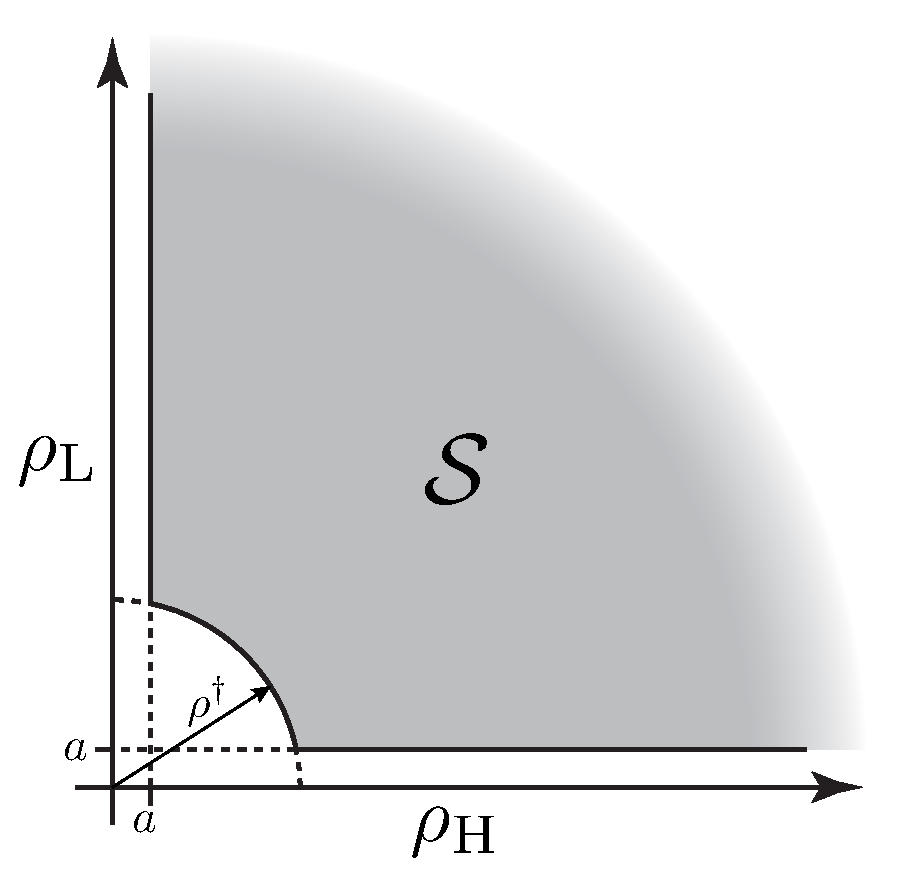
\includegraphics[height=4.25in]{figures/SNRintegrationRegion.pdf} \\
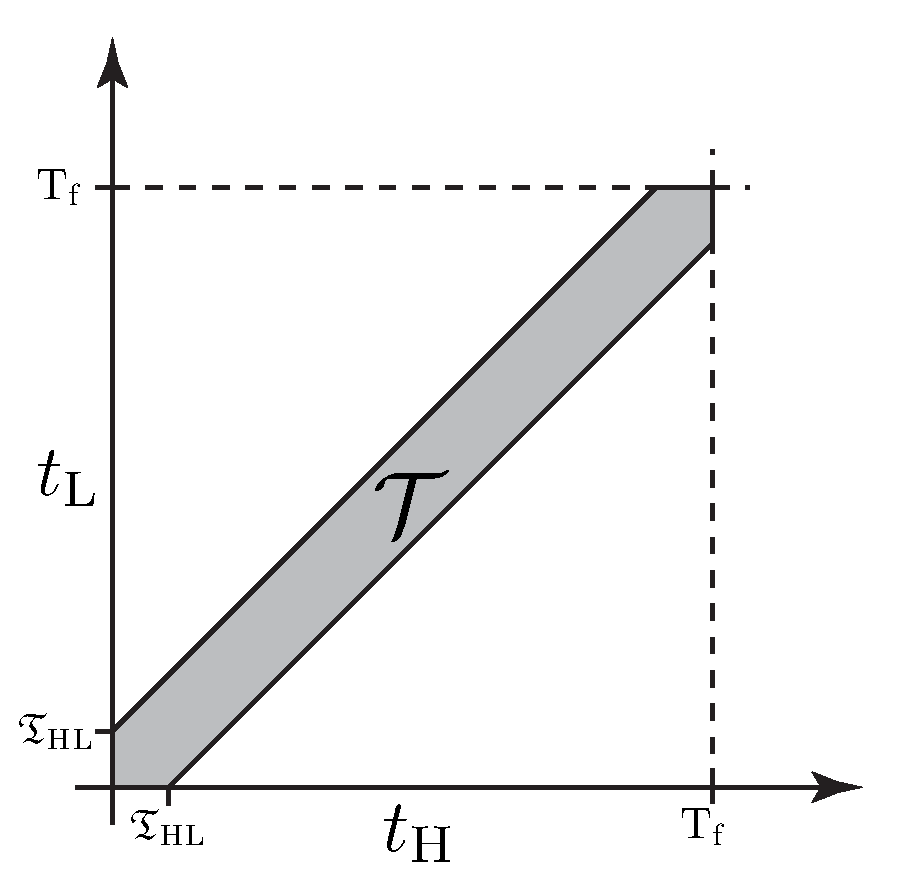
\includegraphics[height=4.25in]{figures/TimeIntegrationRegion.pdf}
\end{center}
\caption{The regions of integration in $\rho$, and time for a network of two detectors, $\varH$ and $\varL$.}
\end{figure}

\if{false}
For example, if we have two arbitrary detectors, $\varH$ and $\varL$, each with two independent sources $\gamma$ and $\delta$, then equation \ref{eqn:N_rate_general} would be:

\begin{eqnarray}
\label{eqn:exampleSources}
\lefteqn{ \mathbb{E}\left(N_{\mathrm{uncorr}}(\rho^{\dagger2} \leq \rho_\varH^2 + \rho_\varL^2, \Tf) \right) } \nonumber \\
 & = &  \vT(\mathrm{T_f}) \int_{\rho_\varH^2 + \rho_\varL^2 \geq \rho^{\dagger2}}  \d \rho_\varH \d \rho_\varL \times \nonumber \\
 & & \left(\rsrc_{\varH,\gamma}P_{\varH,\gamma}(\rho_\varH) + \rsrc_{\varH,\delta}P_{\varH,\delta}(\rho_\varH)\right) \left(\rsrc_{\varL,\gamma}P_{\varL,\gamma}(\rho_\varL) + \rsrc_{\varL,\delta}P_{\varL,\delta}(\rho_\varL)\right) \\ 
 & = & \coincT_{\varH\varL}(2\Tf - \coincT_{\varH\varL})\int_{\rho_\varH^2 + \rho_\varL^2 \geq \rho^{\dagger2}}  \d \rho_\varH \d \rho_\varL \times \nonumber \\
 & & \{ \rsrc_{\varH,\gamma}\rsrc_{\varL,\gamma}P_{\varH,\gamma}(\rho_\varH)P_{\varL,\gamma}(\rho_\varL) + \rsrc_{\varH,\gamma}\rsrc_{\varL,\delta}P_{\varH,\gamma}(\rho_\varH)P_{\varL,\delta}(\rho_\varL) + \nonumber \\
 & & \rsrc_{\varH,\delta}\rsrc_{\varL,\gamma}P_{\varH,\delta}(\rho_\varH)P_{\varL,\gamma}(\rho_\varL) + \rsrc_{\varH,\delta}\rsrc_{\varL,\delta}P_{\varH,\delta}(\rho_\varH)P_{\varL,\delta}(\rho_\varL) \}
\end{eqnarray}

\section{Computing Background Using Time Slides}

Since we wish to find the \ac{FAR}, $\widetilde{\far}$, and not $\widetilde{\RP}_{\mathrm{all}}$, the second (noise/GWs), third (GWs/noise), and fourth (GWs/GWs) terms above are a problem. Admiting gravitational wave sources into the background will give us a higher rate than the true rate $\widetilde{\far}$. The goal, then, is to remove \acp{GW} when computing the background rate.

This presents a problem: we do not know which triggers are due to gravitational waves and which are not (if we did, we would not have to do all this). Worse, the triggers that we are trying to compute false alarm rates for come from the same distribution of single \ac{IFO} triggers as the background rate that we use. To get around these difficulties, we can employ a few things we know about the physics of gravitational waves.

We know that a gravitational wave will arrive at all \ac{IFO}s within the light travel time between them. Therefore if we add some time offset, $\Delta t$ to each detector that is \emph{greater-than} the light-travel time between it and all other detectors but we only allow coincidences from triggers that are \emph{less-than} $\coincT$:
\begin{equation}
\label{eqn:time_constraint}
|t_i - (t_{i+1}+\Delta t)| \le \coincT_{i,i+1},~\Delta t > \coincT_{i,i+1}
\end{equation}
then we cannot get a coincidence from the same gravitational wave in all detectors. Adding the offset only allows gravitational waves that are coincident with \acp{GW} from other sources into the GWs/GWs term in equation \ref{eqn:mixed_source_terms}. While this can still present a problem, if our time searched is much less than the average rate of gravitational waves in the detectors, then the GWs/GWs term effectively goes to zero.

Adding a time offset has the additional advantage that we can repeat the experiment several times using the same data set to get an average value of $\far$, as long as the offet $\Delta t$ is large enough to ensure that each trial, or \emph{slide}, is independent of each other. The duration of each slide is the union of times that the \acp{IFO} are on after the offsets have been applied. If we do $N_{t}$ slides with each slide having duration $t_{k}$, then from equation \ref{eqn:avg_rate_param} we have:

\begin{equation}
\overline{\far} = \frac{\sum_{k=1}^{N_t} N_k\left(\rho^{\dagger2} \leq \sum_{i=1}^{N_d} \rho_i^2, \vec{\mathcal{O}}_k\right)}{\mathrm{T_{b}}}
\end{equation}
where $\mathrm{T_{b}} = \sum_{k=1}^{N_t}t_k$ is the total \emph{background} time. Here we have made the dependence on the time offset in each slide explicit by defining an \emph{offset-vector}:

\begin{equation}
\vec{\mathcal{O}}_k = \left[\Delta t_1 ~ \Delta t_2 ~ \ldots ~ \Delta t_{N_d} \right]_k %  \{\Delta t_i\}_k,~ i = 1, 2, \ldots, N_d
\end{equation}
which gives the time offsets of each detector in the $k^{\mathrm{th}}$ slide. If all the slides have the same duration, $\tau$, then, from equation \ref{eqn:err_R}, the error in the measurement of $\overline{\far}$ is:

\begin{equation}
\delta \overline{\far} = \frac{1}{\tau}\sqrt{\frac{\sum_{k=1}^{N_t} N_k}{N_t}}
\end{equation}

\section{Bias}
\label{sec:bias}

While the time-slide method gives a better estimate of $\far$, it introduces some bias. To quantify this, consider again equation \ref{eqn:N_general} for all sources. For simplicity, we intially consider only a single coincidence window. In this case, the time integral reduces to:

\begin{eqnarray}
\int_{|t_i - t_{i+1}| \le \coincT_{i,i+1}}^{\mathrm{T}=2\coincT_{i,i+1}}\prod_i^{N_d} \d t_i & = & \int_{-\coincT_{i,i+1}}^{\coincT_{i,i+1}} \prod_i^{N_d} \d t_i \nonumber \\
& = & 2 \prod_i^{N_d} \coincT_{i,i+1} \nonumber
\end{eqnarray}
since all points in time will be within the coincidence window. In the $p\th$ slide, equation \ref{eqn:N_general} becomes:

\begin{equation}
\mathbb{E}\left(N_{\mathrm{all}}(\rho^{\dagger2} \leq \sum_i\rho_i^2, 2\coincT )\right) = \int_{\sum_i\rho_i^2 \geq \rho^{\dagger2}} \prod_i^{N_d} \mathbb{E}\left(n_{i,\mathrm{all}}(\rho_i,t_i + \mathcal{O}_p[i] \pm \coincT_{i,i+1} ) \right) \d\rho_i
\end{equation}
To further simplify the problem, we consider the case in which $\rho^\dagger$


If we performed $N_t$ \emph{independent} experiments, then the expected number of triggers in this window would be:

\begin{equation}
\label{eqn:ideal_slides}
N_t \int_{\sum_i\rho_i^2 \geq \rho^{\dagger2}} \d \rho_i \prod_{i}^{N_d} \mathbb{E}( n_{i,\mathrm{all}}(\rho_i, t_i \pm \coincT_{i,i+1}) ) = N_t \int_{\sum_i\rho_i^2 \geq \rho^{\dagger2}} \d \rho_i \prod_{i}^{N_d} \sum_{k=1}^{\infty} k P(k|i,\mathrm{all}; \rho_i, t_i \pm \coincT_{i,i+1})
\end{equation}
When we perform time-slides, however, each of the slides are not truly independent. To see why, focus on one of the detectors, call it $\varH$, against which the other detectors are slid. In the first slide, the integrand is equation \ref{eqn:ideal_slides} (with $N_t = 1$). In each subsequent slide, the same expression will hold for all detectors aside from $\varH$, since, by sliding, we have introduced new data into the coincidence window. Yet because we are using the \emph{same} data in $\varH$, the probability of getting $k$ triggers in $\varH$ is \emph{not} $P(k|\varH,\mathrm{all}; \rho_i, \tau)$; instead, it is one if $k = n^{(0)}_{\varH}$ --- where $n^{(0)}_{\varH}$ is the number of triggers that occurred in $\varH$ in the first slide --- and zero otherwise. In other words, the \ac{PDF} in $\varH$ has collapsed around $n^{(0)}_\varH$. The expected number in the coincidence window is thus:

\begin{equation}
\label{eqn:actual_slides}
N_t \left(\prod_{i \neq \varH} \sum_{k=1}^{\infty} k P(k|i,\mathrm{all}; \rho_i, t_i \pm \coincT_{i,i+1})\right) \sum_{k=1}^{\infty} k \delta^{k}_{n^{(0)}_\varH} = N_t \prod_{i \neq \varH}^{N_d} \mathbb{E}( n_{i,\mathrm{all}}(\rho_i, t_i \pm \coincT_{i,i+1}) ) n^{(0)}_\varH
\end{equation}



%%%%%%%%%%%%%%%%%%%%%%%%%%%%
\if {false}
$m^{\mathrm{th}}$ noise source in the \varH~ detector and the $n^{\mathrm{th}}$ noise source in \varL. Let the true rate densities of these noise sources be $\widetilde{r}_{\varH,m}$ and $\widetilde{r}_{\varL,n}$, respectively. At a given time $t$, we will get a coincident trigger if there is at least one trigger from each source within $\coincT_{\varH\varL}$. The probability of getting atleast one coincident trigger is therefore:

\begin{eqnarray}
P(N_c \geq 1 | \widetilde{\rsrc}_{\varH,m}, \widetilde{\rsrc}_{\varL,n}, t \pm \coincT_{\varH\varL} ) &  & \nonumber \\
 & = & P(N \geq 1 | \widetilde{\rsrc}_{\varL,m},t \pm \coincT_{\varH\varL})P(N \geq 1 | \widetilde{\rsrc}_{\varL,m}, t \pm \coincT_{\varH\varL}) \nonumber \\
 & = & \left( 1 - e^{-\widetilde{\rsrc}_{\varH,m}2\coincT_{\varH\varL}} \right)\left( 1 - e^{-\widetilde{\rsrc}_{\varL,m}2\coincT_{\varH\varL}} \right)
\label{eqn:true_coinc_prob}
\end{eqnarray}
In equation \ref{eqn:true_coinc_prob} we have used the fact that the probability of getting one or more events from a Poisson distribution is:

\begin{eqnarray}
P(N \geq 1 | \RP, \tau) & = & 1 - P(0|\RP,\tau) \nonumber \\
    & = & 1 - e^{-\RP\tau}
\end{eqnarray}

Within a single slide, each block of coincident time can be considered to be an independent measure of the coincident $m,n$ rate density $\far_{m,n}$. Assuming $\far_{m,n}$ is constant across the duration of the slide, $\tau$, then we have $\tau/\coincT_{\varH\varL}$ measures of $\far_{m,n}$. However, this will not be sufficient to get a good approximation of $\widetilde{\far}_{m,n}$ especially if:

\begin{equation}
\widetilde{r}_{\varH,m}\widetilde{r}_{\varL,n} \left(\frac{\tau}{\coincT_{\varH\varL}}\right) < \frac{1}{\coincT_{\varH\varL}^2}
\end{equation}
In this case the expected number of events across the slide would be less than 1, making it likely that we would record no value and therfore end up with a mean value of zero for $\overline{\far}_{mn}$. For this reason, we extend the number of measures of $\far_{mn}$ we have by adding more slides.

However, the slides are not true indepedent measurements. Consider the same point in time in the $\varH$ detector as before, but now in the next slide. If this was a truly independent measurement, then the probability of getting one or more coincident triggers would again be equation \ref{eqn:true_coinc_prob}. The probability of getting a trigger during this period of time in $\varL$ would be the same it has been slid a period of time greater than $\coincT_{\varH\varL}$. The probability of getting a trigger in $\varH$, however, is \emph{not} the same. Since we are using the exact same period of time, it will be either 0 or 1, depending on whether or not we got a trigger in the first slide. Thus, the probability of getting a trigger at time $t$ for this and all subsequent slides is:

\begin{eqnarray}
P(N \geq 1|\widetilde{\rsrc}_{\varH,m}, \widetilde{\rsrc}_{\varL,n}, t \pm \coincT_{\varH\varL}, \mathcal{O}_{k \neq 1}) &  \nonumber \\
 = & \left\{
\begin{array}{l l}
1 - e^{-\widetilde{\rsrc}_{L,n}\coincT_{\varH\varL}} & \mbox{if $N_{\varH,m}(\mathcal{O}_1) \geq 1$} \\
0 & \mbox{if $N_{\varH,m}(\mathcal{O}_1) = 0$}
\end{array}
\right.
\end{eqnarray}

\fi
%In our ideal world of independent measurements, the probability that we will get atleast one coincident trigger with $\rho_c^2 \geq \rho^{\dagger2}$ at a time $t$ is given by the probability that we get one or more trigger in each detector within $\coincT$:

%\begin{equation}
%P(N \geq 1 | t, \{\widetilde{r}_{i,j}\}) = \prod_{i = 1}^{N_d} P(N \geq 1 | t\pm\Delta \coincT_{i}, \widetilde{r}_{i,n_i})
%\end{equation}

\fi

\end{document}


\Chapter{The IHOPE Pipeline}
\label{ch:ihope_pipeline}
% ihope_pipeline.tex

% citation shortcuts
\def\12to18{Abbott:2009qj}
\def\sfive1yr{Collaboration:2009tt}
\def\sfivelvc{S5LowMassLV}


In this chapter we describe in detail the \ihope pipeline, which is the pipeline
used to carry out the \ac{CBC} search. This pipeline has been used to analyze
data taken from \ac{S5} \cite{\sfive1yr,\12to18}, \ac{S6}, \ac{VSR2}, and
\ac{VSR3} \cite{s6paper}.

\ihope can by modeled by a \ac{DAG}. A \ac{DAG} is a workflow in which the
output of one program, or {\it node}, is the input of another node or nodes,
such that the flow never loops back onto itself. It is represented by a diagram
in which the vertices are the programs and the edges show the interdependencies
\cite{condor}. \ihope is a \ac{DAG} of \ac{DAG}s: its nodes are workflows that
launch sub-workflows, which in-turn launch the programs that carry out the
analysis. These \ac{DAG}s are managed by the Condor High Throughput Computing
system, which distributes the jobs across the computer cluster and manages the
dependencies. Figure \ref{fig:ihopeOverview} shows an overview of the \ihope
workflow. Data from each \ac{IFO} is retrieved, analyzed in parallel workflows,
combined, and then output to a webpage. Each of these steps involves one or
more \ac{DAG}s.

In this chapter we go through each of these steps in detail. Section
\ref{sec:PipelineRequirements} reviews the requirements of a \ac{CBC} \ac{GW}
pipeline; section \ref{sec:ihopeRuntime} explains how the dag is set-up at
run-time; section \ref{sec:HIPEdetail} describes the HIPE pipeline in detail;
\ref{sec:TableStructure} describes the tables used to store data;
\ref{sec:PipedownDetail} describes Pipedown in detail and how the results are
presented. 

\begin{figure}[h]
\begin{center}
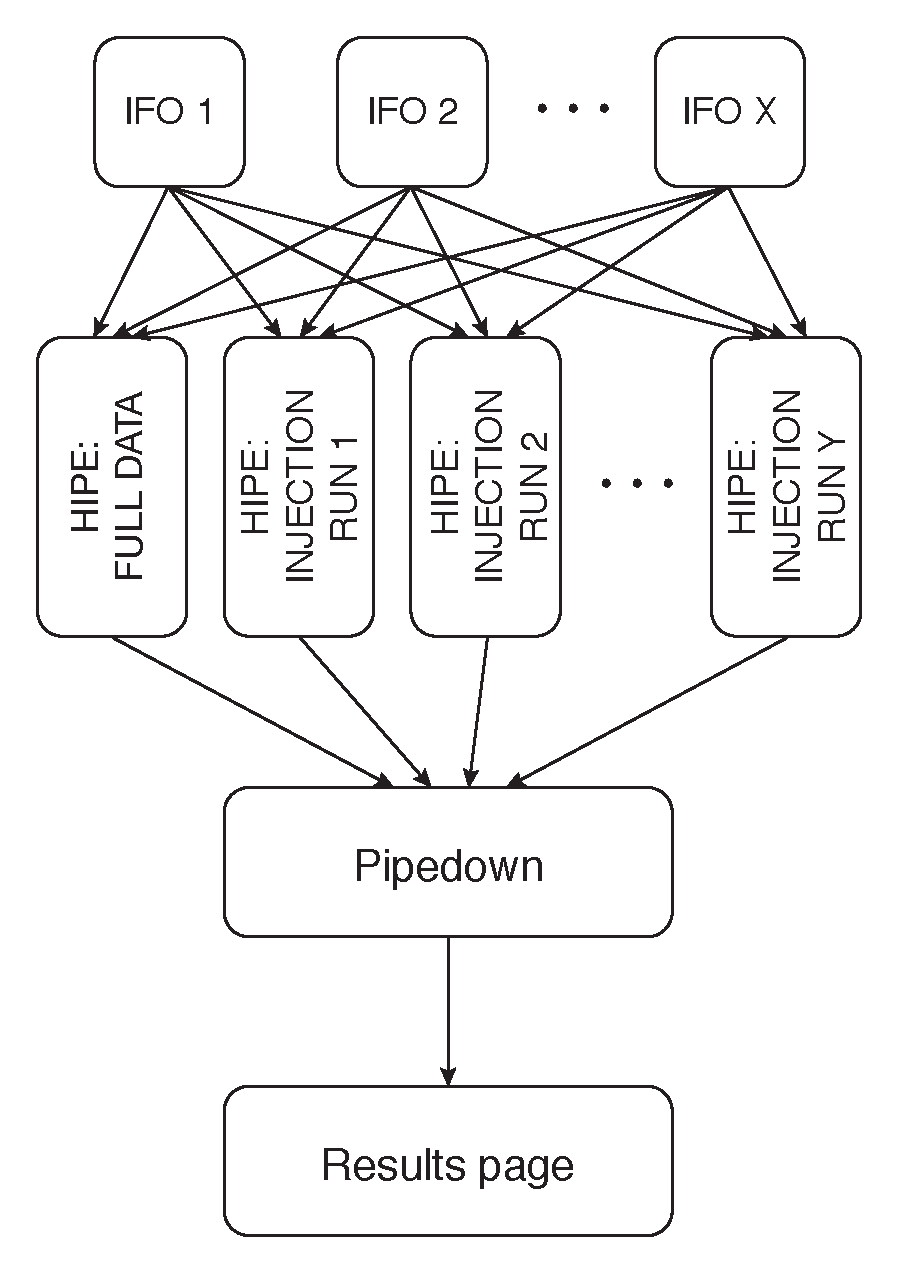
\includegraphics[width=2.5in]{figures/ihopeOverview.pdf}
\end{center}
\caption{
An overview of the \ihope pipeline. The HIPE and Pipedown nodes are themselves workflows, and are detailed in later sectionss.
}
\label{fig:ihopeOverview}
\end{figure}

\section{Pipeline Requirements}
\label{sec:PipelineRequirements}

Before delving into the details of \ihope, we briefly review the key
requirements of a pipeline used to search for \ac{GW}s. Our goal is to search
for \ac{GW}s from coalescing binaries in a range of masses. Hampering our
efforts is the fact that gravitational waves couple very weakly to matter; we
must be able to detect strains of $\sim10^{-21}$. Despite this, we
aim to detect at a \ac{SNR} of $8$ in each detector to ensure statistical
confidence in our search.

When averaged over time the detectors' have a colored-Gaussian noise
distrubtion; as shown in Chapter \ref{ch:pipeline_principles}, the best analysis tool to search for signals is therefore a
matched filter \cite{?}. Match filtering requires knowing the morphology of the
waveform. Fortunately, binaries with total masses (\mtotal) less than $25\Msun$
sweep through the \ac{LIGO} and Virgo bands during their {\it inspiral} phases.
This means that the waveform from these systems can be well modelled by the
post-Newtonian approximation. For higher-mass systems ($25 < \mtotal/\Msun <
100$), in which the merger and ringdown part of the waveform become important,
numerical relativity waveforms can be stiched to the \ac{pN} approximation;
phenomenological waveforms may also be used. Thus, to cover the desired range,
we can fill a bank of templates using the methods described in section \ref{sec:multiple_templates} of Chapter \ref{ch:pipeline_principles}.

Environmental and instrumental factors can cause non-Gaussian transient noise
(\emph{glitches}) in the data. To deal with this our pipeline must be able to
distinguish between triggers resulting from glitches and triggers resulting
from gravitational waves. Since the morhpology of the signals is known, the $\chi^2$ test discussed in \ref{ch:pipeline_principles} lends itself as a good method to do this. Checking for coincident triggers in multiple detectors will
also filter out spurious triggers since we do not expect environmental
correlations across great distances. After all filtering and tests have been
applied, the statistical significance of a set of triggers has to be evaluated
to determine the probability that a gravitational wave exists in the data. A
pipeline must therefore be able to compute a background with which to compare
triggers to. To avoid bias, this must be done in a {\it blind} fashion: the
method by which background is chosen and triggers ranked must be chosen without
knowledge of what is in the data, else the results will sway in the favor of the
analysts' bias. 

Finally, the pipeline must be able to evaluate its sensitivity and efficiency
to sources in the universe. Doing so allows tuning studies to be carried out
prior to doing the full analysis, and for the astrophysical rate of \ac{CBC}s
to be bounded after the analysis has completed. This can be done by performing
\emph{injections} of signals with known parameters into the detectors. Both \emph{hardware} and \emph{software} injections may be performed. Hardware injections
involve actuating the mirrors to physically simulate a passing gravitational
wave. This is the most robust test as it checks the ability of the detectors'
response loop to measure \ac{GW} strains and the ability of the pipeline to
detect them. The trouble with hardware injections is that real \ac{GW}s cannot
be detected while they are occurring, limiting the number that can be done.
Software injections involve adding a gravitational wave signal to the data
stream on disk just prior to analyzing it. While this method doesn't test the
hardware control systems, it has the advantage that it can be done many times
in parallel, without corrupting the original data. Thus, our pipeline must be
able to perform software injections, and have a method for associating triggers
with the injections that went into the data.

In summary, a pipeline used to search for gravitational waves from \ac{CBC}s must:
\begin{itemize}
\item{construct a bank of templates with which to filter;}
\item{identify \emph{triggers} by filtering templates through the detector data;}
\item{distinguish noise triggers from gravitational wave triggers;}
\item{quantify statistical significance of triggers and rank them in a blind manner;}
\item{evaluate the sensitivity and efficiency of the search to \ac{CBC}s in the universe.}
\end{itemize}
In the following sections we will see how \ihope meets these requirements.


\section{\ihope at Runtime}
\label{sec:ihopeRuntime}

The \ihope pipeline is created by running \texttt{lalapps\_ihope}. This sets up
the workflow by doing the following at run time:

\begin{itemize}
\item{set-up the directory structure to save all data to;}
\item{copy all needed programs from their installed location to a local directory;}
\item{retrieve analysis start and stop times;}
\item{download a {\it veto-definer file} and find the start and stop times of all veto segments;}
\item{run \texttt{lalapps\_inspiral\_hipe};}
\item{run \texttt{lalapps\_cbc\_pipedown};}
\item{create a cache file of the names and locations of all files that will be created;}
\item{write a DAX that can be used to start and run the worflow.}
\end{itemize}

These steps require the start and stop time (in GPS seconds) of the period to
be analyzed as well as a configuration file. The configuration file is a text
file containing all the information needed to setup and run the analysis. This
includes: the names and locations of all the executables that will be run;
variable arguments that these programs will need; the name and number of
interferometers to analyze; the version of data files to retrieve and what
channels to analyze; how many and what type of software injection runs to do;
any other information needed by the \ac{DAG}s to run. The configuration file
provides a convenient way to manipulate the pipeline. Changing tuning
parameters is largely accomplished by editing this file. Likewise, the
difference between running a {\it low-mass} search ($2 < \mtotal/\Msun < 25$)
and a {\it high-mass} search ($25 < \mtotal/\Msun < 100$) is determined
entirely by the configuration file.

A directory named by the gps start/stop times is created at runtime. All work
is done in this directory. In it, a \texttt{segments}, \texttt{executables},
\texttt{datafind}, \texttt{full\_data}, and \texttt{pipedown} directory are
created, along with a directory for each injection run that will be carried
out. With the exception of the \texttt{executables} and \texttt{segments}
directory, each of the sub directories store a sub-\ac{DAG} that will be run
during the analysis (and will be explained below). The master \ac{DAG} is saved
in the gps-times direcotory along with a master cache file of all the files
that will be created. All programs that will be run are copied to the
\texttt{executables} directory.

\subsection{Science and Veto Segments Retrieval}

The \ac{LIGO} and Virgo detectors can be in one of five different states at any
given time. We are only interested in analyzing times in which the detectors
are in {\it Science} mode. This means they are up, locked, and no other
experimental work is being done on them \cite{?}. The interferometers
can drop out of Science mode many times across an analysis period; thus \ihope
must retrieve the start and stop times of Science segments that occurred in the
desired analysis period. \ihope does this by running
\texttt{ligolw\_segment\_query} at run time. This program queries the {\it
segment database} --- a remote database that contains lists of segments
detailing the times that each of the detectors were in various states --- to
retrieve the list of Science times during the desired analysis period. These
results are saved to xml files in the \texttt{segments} directory. These files
do not contain strain data; they only list the times that data can be
retrieved. The results are later used to retrieve files containing strain data.

Various environmental and instrumental factors can cause periods of elevated
glitch rate during Science mode. If these periods are analyzed with periods of
relatively clean data, they will pollute the background estimation, thereby
decreasing statistical confidence in candidates. We therefore seek to remove
such periods from the analysis. This is accomplished using vetoes. Vetoes are
categorized according to how well we can couple them to known environmental
sources; they are applied cumulatively. Table \ref{tab:vetocats} lists the
various categories and their defining characteristics. For \ac{CBC} searches,
we do not analyze anything prior to category 1; i.e., all matched filtering is
done after category 1 vetoes are applied. Category 2 and 3 vetoes are applied
when second stage coincidence is carried out (see HIPE, below). We quote false
alarm rates and base upper limits on data in which category 1-3 vetoes have
been applied. We additionally check the data after category 1 and 2 vetoes have
been applied for any loud triggers that may have been removed by category 3
vetoes. We do not use category 4 for the anlaysis; however, we do use them in
follow-up studies of loud events to provide insight into the cause of the
events. Hardware injections are left in the data after category 1 and 2, and
are removed as a special veto prior to category 3 vetoes being applied.

\begin{table}
\center
\begin{tabular}{c | p{5cm} | p{8cm}}
Category    &    Description    &   Procedure    \\
\hline
    1       &    Data seriously compromised or missing.    &    Data never analyzed. \\
\hline
    2       &    Instrumental problems with known coupling to h(t).    &    Vetoed triggers discarded after second coincidence. Surviving triggers checked for candidates, but not used for upper limits. \\
\hline
    3       &    Instrumental problems likely, casting doubt on triggers found during these times.    &    Vetoed triggers discarded after second coincidence. False alarm rates of surviving triggers are used in publications; upper limits are calculated using these vetoes.  \\
\hline
    4       &    Positive, but weak, correlations with false alarms. Large dead times.    &     Not used in the analysis, but used as a guide in detailed followups of loud triggers. \\
\end{tabular}
\caption{The various veto categories used by the \ac{CBC} group. Vetoes are applied cumulatively; statistical significance of candidates and upper limits are calculated after category 1, 2, and 3 vetoes are applied.}
\label{tab:vetocats}
\end{table}

Vetoes are triggered by environmental and instrumental channels that flag
various segments of time for suspicious activity. Additional flags can be added
by hand; e.g., if a truck drives onto the site during Science mode, a person
in the control room may add a flag for that period of time. All of these flags
are stored in the segment database. What flags to use for vetoes, at what
category, and for how long, are stored in a \emph{veto-definer file}. This xml
file contains a \texttt{veto\_definer} table that lists each flag that should
be used, what category the flag should be used at, the dates the flag is valid, and any
padding (in seconds) to add to the flag should it go off. Entries are added to
this table by hand after extensive data-quality investigations and safety
checks. Vetoes are fine tuned for specific searches and epochs, and each
searches' set is saved in a different veto-definer file in a central
repository. What veto definer file to use is specified in the \ihope
configuration file. At run-time, \ihope downloads the desired file to the
\texttt{segments} directory. It then runs \texttt{ligolw\_segments\_from\_cats}
to query the segment database for flags specified in the veto-definer file. The
vetoed segments for all of the instruments are added together and saved in xml
files in the \texttt{segments} directory.


\subsection{HIPE}

Once the analyzable Science segments and the veto segments that will be applied
are obtained, \ihope runs \texttt{lalapps\_inspiral\_hipe}. This sets up the
\ac{HIPE}, which is the pipeline that carries out the search. Figure
\ref{fig:HIPEDiagram} shows the \ac{HIPE} \ac{DAG} for a single $2048\rm{s}$
block of time. \ac{HIPE} can be run both with and without injections. If
injections are being done, \texttt{lalapps\_inspinj} is run to create a list of
injections to make, which are created and inserted into the data just prior to
match filtering by \texttt{lalapps\_inspiral}.

As can be seen in Figure \ref{fig:ihopeOverview}, \ihope runs \ac{HIPE} several
times: once for zero-lag and time-slid data (which we label
\texttt{FULL\_DATA}), and once for each desired injection run, which are
specified in the configuration file. The details of the steps of this analysis
are discussed in Section \ref{sec:HIPEdetail}.

%
%\if{false}
%The playground run is done so we may tune the pipeline while keeping the analysis blind. We have designated 600 of every 6370 seconds of data as playground. This data is looked at prior to un-blinding the analysis (what we colliquoly call \emph{opening the box}) in order to tune vetoes and check for any spurious data that would indicate a bug in the analysis. Although playground data is included in the final open-box analysis, we exculde it for computing upper-limits. Note that playground zero-lag data can easily be retrieved from the \texttt{FULL\_DATA} analysis -- we can simply filter triggers based on their end-times for the playground times. The real difference between the \texttt{FULL\_DATA} analysis and the \texttt{PLAYGROUND} analysis is in the time-slides: \texttt{PLAYGROUND}...
%\fi
%

\begin{figure}[p]
\begin{center}
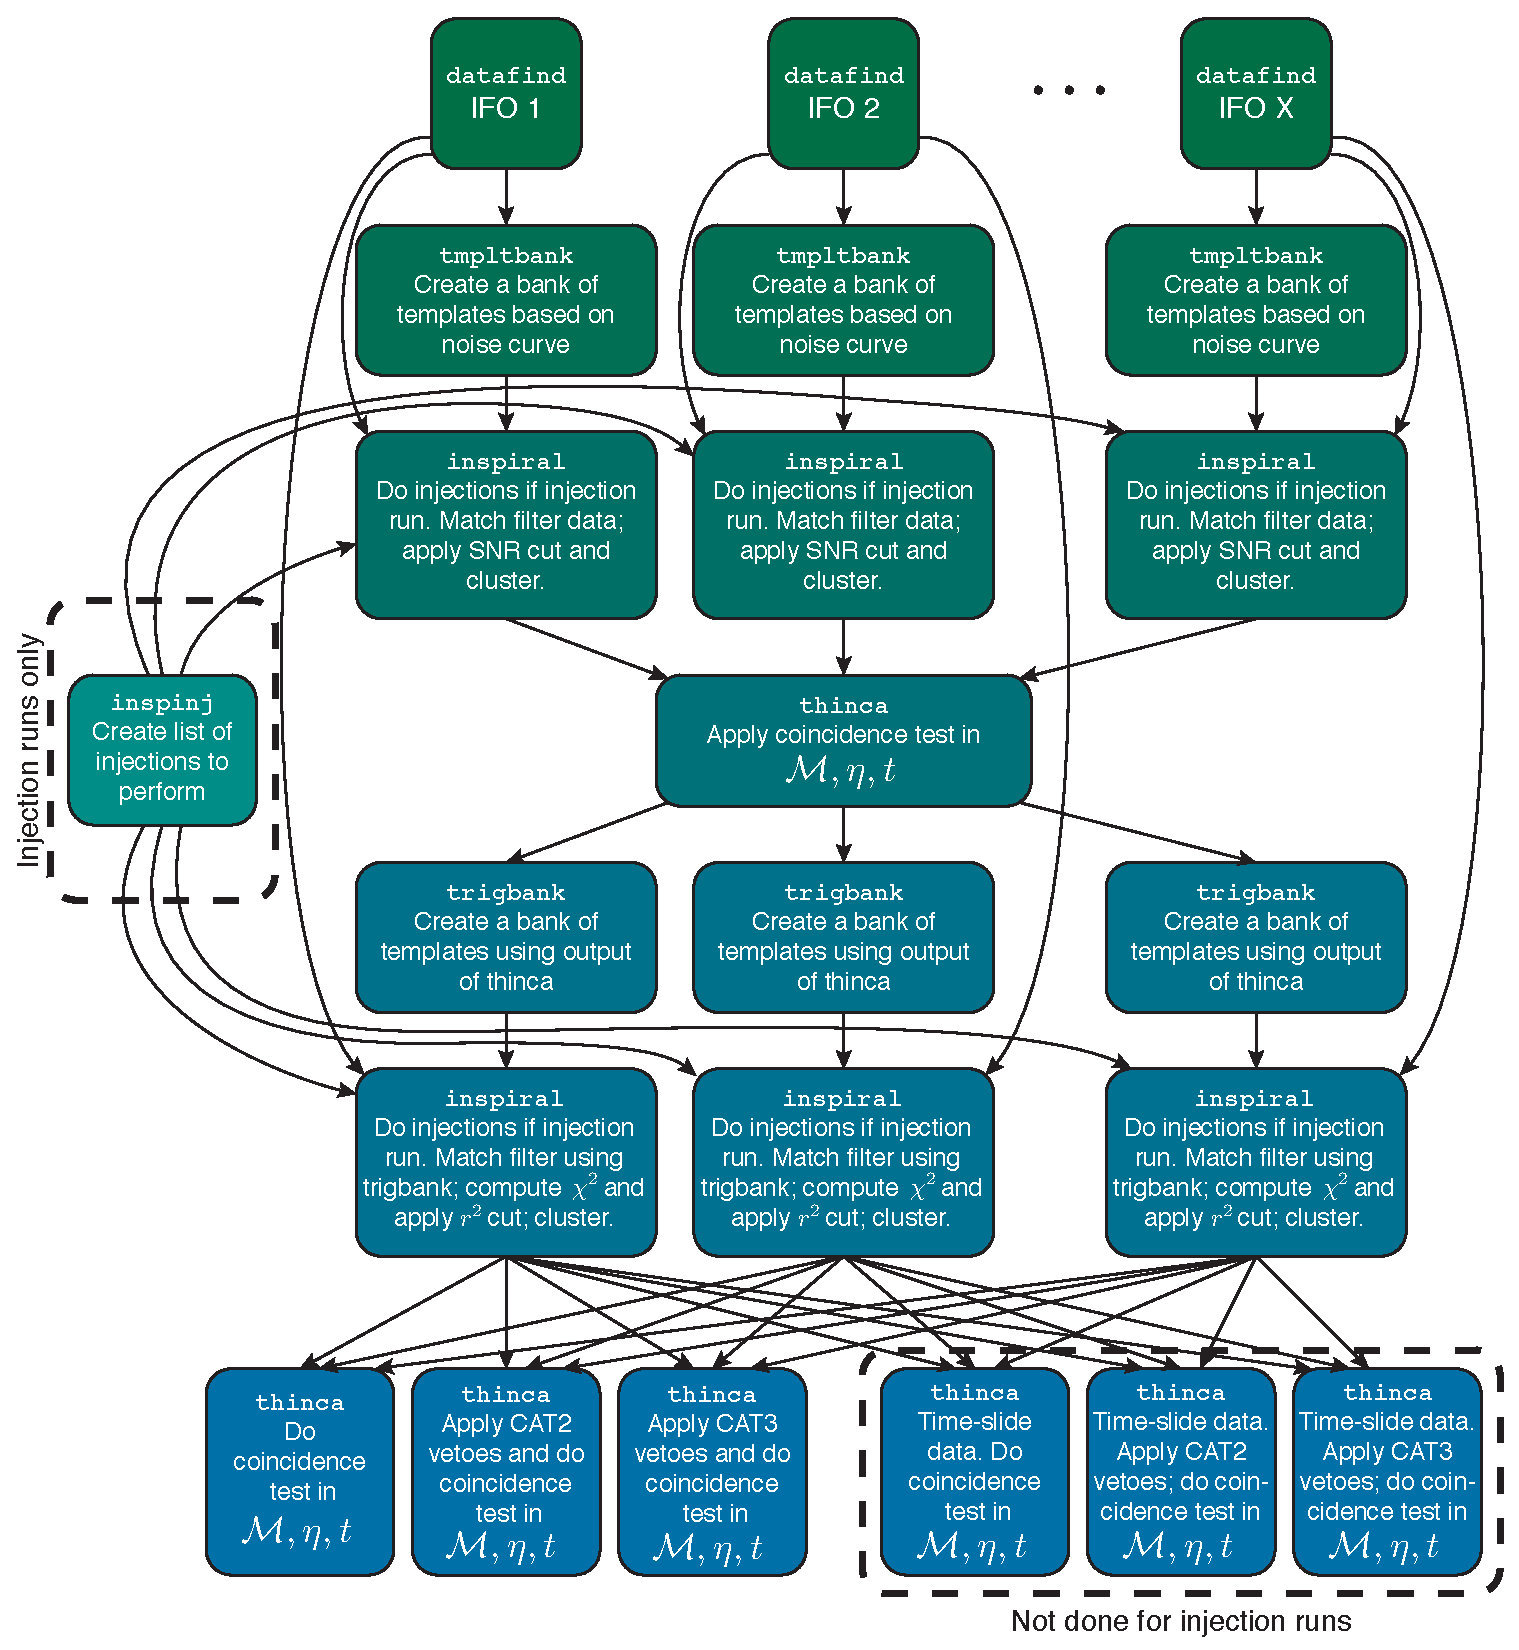
\includegraphics[width=6in]{figures/HIPEDiagram.pdf}
\end{center}
\caption{
The \ac{HIPE} pipeline. This is run once for full-data and once for
each injection run. For injection runs, \texttt{lalapps\_inspinj} is run to
generate a list of injections to create, and time slides are not done.
}
\label{fig:HIPEDiagram}
\end{figure}

\subsection{Pipedown}

After all the instances of \texttt{lalapps\_inspiral\_hipe} have run, \ihope
run \texttt{lalapps\_cbc\_pipedown} which sets up the Pipedown \ac{DAG}.
Pipedown takes the results of all the different HIPE runs, combines them into
SQLite databases, computes and ranks triggers by \ac{FAR}, and creates plots
and tables of the results. Figure \ref{fig:PipedownDiagram} details the steps
Pipedown takes to carry out these goals. Shown are the steps taken for a single
veto-category; this diagram is repated for each veto-category (by Pipedown, not
by \ihope). In-depth details of Pipedown are discussed in Section
\ref{sec:PipedownDetail}.

\begin{figure}[p]
\begin{center}
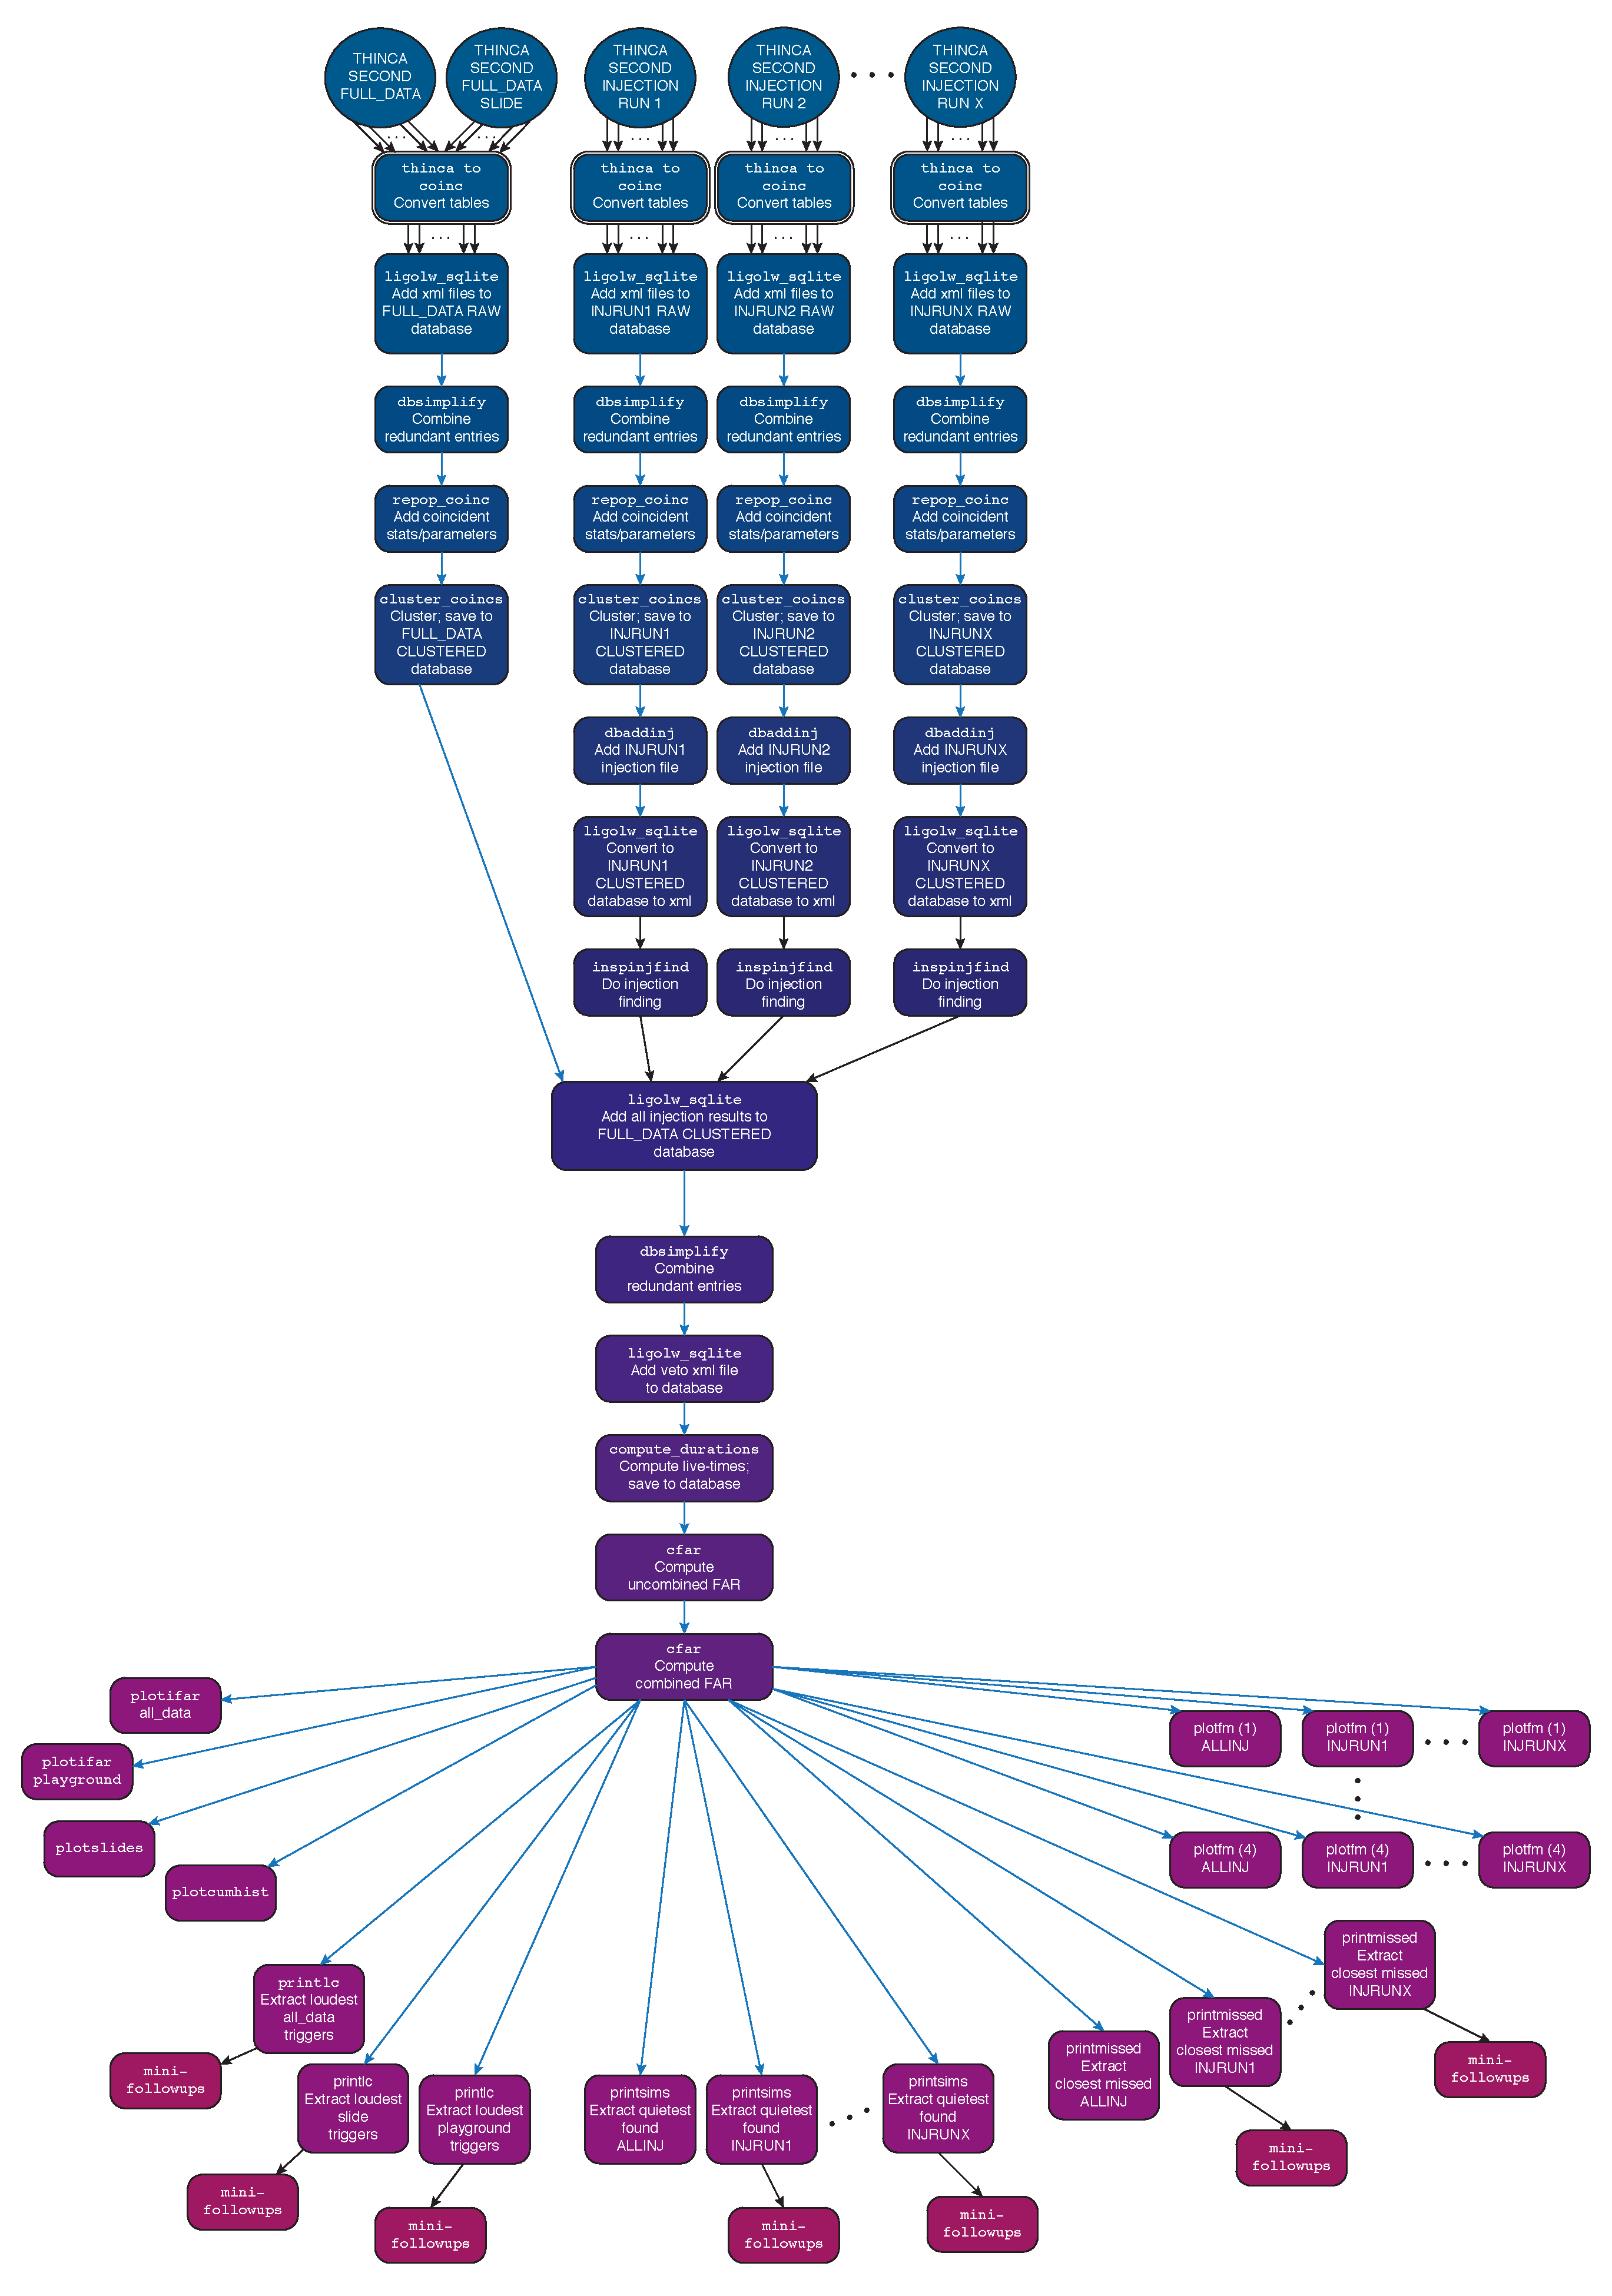
\includegraphics[width=5in]{figures/PipedownDiagram.pdf}
\end{center}
\caption{
The Pipedown pipeline for a single veto category. Each block represents a single node. Double bordered blocks represent multiple nodes. Circles represent batches of files. Black arrows represent xml files; blue arrows, SQLite databases. Each arrow represents a single file.
}
\label{fig:PipedownDiagram}
\end{figure}

\subsection{DAX}

After pipedown has completed, \ihope writes a DAX that can be used to launch the pipeline. A DAX is an abstract workflow in which elements such as file locations are variables. The DAX is turned into a \ac{DAG} by the Pegasus Workflow Management Service.

\section{HIPE in Detail}
\label{sec:HIPEdetail}

We now step through \ihope in detail, using a toy analysis of $10,240$s as an example. In this analysis we will use three interferometers: the 4-kilometer Hanford detector (H1), the 4-kilometer Livingston detector (L1), and the 3-kilometer Virgo detector (V1), and we will add one injection run, which we label \texttt{BNSINJ}. Figure \ref{fig:science-selected_segs} shows the segments that are available to analyze during this time. The \emph{selected segments} are Science segments minus CAT1 veto segments; they are what \ihope passes to \ac{HIPE} to analyze.

\begin{figure}[p]
\begin{center}
\includegraphics[width=5in]{figures/segment_plot_science-selected.pdf}
\end{center}
\caption{
The Science, category 1 vetoes, and selected segments of H1, L1, and V1 between GPS times 967228343 and 967238583.
}
\label{fig:science-selected_segs}
\end{figure}


\subsection{Data Find}

As can be seen in Figure \ref{fig:HIPEDiagram}, the first step in \ac{HIPE} is to run \texttt{lalapps\_data\_find}. Data from all of the interferometers are stored in \emph{frame files} in central locations at every computer cluster. Frame files can contain multiple channels recorded from the interferometers. For analysis purposes, we are only interested in files containing the strain data channel, which is called \texttt{LDAS-STRAIN} in the \ac{LIGO} detectors and \texttt{h\_16384Hz} in Virgo. \texttt{lalapps\_data\_find} finds the files covering the selected segments on the cluster and creates cache files listing the location of each these files in the \texttt{datafind} directory. These cache files are passed to \texttt{lalapps\_tmpltbank} and \texttt{lalapps\_inspiral}, which use them to locate and open the frame files for analysis.

\subsection{PSD Estimation and Data Segmentation}

\texttt{lalapps\_inspiral} is the program that constructs the \ac{SNR} time series for templates laid out in a bank by the program \texttt{lalapps\_tmpltbank}. The \ac{SNR} time series is constructed according to equation \ref{eqn:snr_full_form} and the templates are laid out using the metric defined in equation \ref{eqn:templateMetric}. Since both of these equations involve the inner product defined in equation \ref{eqn:inner_product}, both programs must compute the \ac{PSD}, $S_n(|f|)$, as well as the Fourier Transform of the data, $\widetilde{s}(f)$. (We do not Fourier Transform the templates. Instead, we generate the templates in the frequency domain directly by using the \ac{SPA}.)

So far, all equations we have used involving Fourier Transforms and the inner product have assumed continuous time- and frequency-domain data series. Likewise, the integrals over frequency space have been from $-\infty$ to $+\infty$. In practice, of course, the data is discreetly sampled and is neither continuous nor infinite. Both the \ac{LIGO} and Virgo strain data are sampled at $16,384\,\mathrm{Hz}$. Since even the lowest mass templates (i.e., waveforms with the highest frequency components) used in current \ac{CBC} searches terminate at frequencies around a couple of kHz, this sampling rate is much finer than is needed for our purposes. To ease computational requirements the time series is therefore downsampled to $4096\,\mathrm{Hz}$ in both \texttt{lalapps\_inspiral} and \texttt{lalapps\_tmpltbank} prior to analysis. This sampling rate sets the Nyquist frequency, $f_{\mathrm{Nyquist}}$, at $2048\,\mathrm{Hz}$. To prevent aliasing, a low-pass time-domain digital filter with a cutoff at $f_{\mathrm{Nyquist}}$ is implemented to pre-condition the data. On the low-frequency end, seismic noise dominates the interferometers' power spectrum. We therefore also impose a high-pass digital filter in the time domain. The cutoff frequency of the high-pass filter, $f_c$, is set to be a several Hz lower than a low-frequency cutoff, $f_0$, that is determined by the characteristics of each \ac{IFO}'s power spectrum. These values are set in the configuration file. (For the values chosen for \ac{S5} and \ac{S6} see Chapters \ref{ch:s5_results} and \ref{ch:s6_results}, respectively.) Both the low and high-pass filters will ring at the start and end of a time series, corrupting the data. Thus we must remove the first and last $t_{\mathrm{pad}}$ of data after applying the filters and prior to analyzing. The duration of $t_{\mathrm{pad}}$ is also set in the configuration file; for both \ac{S5} and \ac{S6} we used $8\,$s.

To Fourier Transform the data, we use the \ac{FFT} algorithm. The \ac{FFT} imposes two constraints on the data. First, the number of points in the data series must be a power of two. Second, the \ac{FFT} associates the last point of the data series with the first point; i.e., it wraps the data around on a loop. This means that as a template is slid toward the end of the time series, any points extending beyond the end of the series will be placed at the beginning. Additionally, because the last and first point of the time series are discontinuous, the wrap around essentially introduces a delta function at the end of the series. As the template passes past the discontinuity it will ring (i.e., the match filter will return the template's impulse response), and, due to the wrap around, this ringing will be placed at the beginning of the time series. Thus the first $t_{\mathrm{chirp}}$ points of the \ac{SNR} time series are corrupted, where $t_{\mathrm{chirp}}$ is the \emph{chirp length} of the template, and must be thrown out.

The chirp length is defined as the length of time it takes for the binary to go from $f_0$ to the frequency at which the binary passes \ac{ISCO}, $f_{\mathrm{isco}}$. \ac{ISCO} is the point when the separation distance is too small for the binary's masses to maintain stable orbits without external energy being added to the system; at this point the masses cease to inspiral and plunge into each other.\footnote{Note that \ac{ISCO} is not the same as the Schwarzschild radius; e.g., in a Schwarzschild space-time, \ac{ISCO} occurs at $r = 6GM/c^2$ whereas the Schwarzschild radius occurs as $r = 2GM/c^2$.} Since the \ac{pN} approximation breaks down at $f_{\mathrm{isco}}$, we must terminate all integrals at this point. Combining this with the realities of Nyquist and seismic noise, all frequency domain integrals are limited to the region $f \in [f_0, f_{\mathrm{max}})$ where $f_{\mathrm{max}} = \min(f_{\mathrm{Nyquist}},~f_{\mathrm{isco}})$.

The \ac{PSD} is estimated using Welch's method. This involves breaking a data segment up into several bins of equal duration. Within each bin, the data is transformed to the frequency domain via the \ac{FFT}. Thus the number of points in each bin must be a power of two, and the bins must be overlapping to account for the wrap-around corruption at the beginning and end of each segment. Since the data is discreet, this results in a discreet number of frequency bins. The \emph{median} value within each frequency bin is then chosen across all the data segments to construct $S_n(|f|)$. We use the medain --- as opposed to the mean --- to better buffer the \ac{PSD} from over-estimation in the prescence of a signal.

As was the case with the template, $S_n(|f|)$ will be corrupted by the discontinuity between the first and last point of the data series. However, unlike the template, which has a finite duration, $S_n(|f|)$ will ring for the entire data segment. This ringing will also happen if a delta-function like glitch exists in the data. To prevent the entire segment from being corrupted, we \emph{truncate} the \ac{PSD}. This is done by estimating \ac{PSD} using Welch's method, inverse transforming $\sqrt{S_n^{-1}(|f|)}$ to the time domain, zeroing out the first and last $t_{\mathrm{invspectrunc}}$ seconds of the time series, then transforming back to the frequency domain. This limits the corruption due to the wraparound to the first and last $t_{\mathrm{invspectrunc}}$ seconds of the time series. The truncation does cause some smoothing out of high Q features, such as power-line harmonics; however, since we search for relatively broad band signals this smoothing has little effect on the search. The value of $t_{\mathrm{invspectrunc}}$ was set to $8\,$s for both \ac{S5} and \ac{S6}.

For more details on \ac{PSD} estimation and implementation of the matched filter with a discreet and finite time-series, see \cite{ref:Brown} and \cite{ref:FindChirp}.

\subsection{Template Bank and Inspiral}

We therefore identify \emph{triggers} by selecting points when $\rho(t)$ is maximum. This is done by using the \emph{max over chirp length} algorithm. Max over chirp length uses a sliding time window to select triggers: for every point in time, a point is only kept if there is no other point with a $\rho$ greater than it within the \emph{chirp length} of the template. $f_0$ is selected based on when the detector's \ac{PSD} effectively goes to infinity due to low-frequency seismic noise. In intial LIGO, $f_0$ is set to $40\,\mathrm{Hz}$; for advanced LIGO it is expected to be $10\,\mathrm{Hz}$. Once a trigger is identified, the time at which it occurs is associated with the \emph{coalescence}, or \emph{end-time}, $t_c$, of the binary.

For \ac{S5} and \ac{S6}, we laid out templates on a hexagonal grid using non-spinning 2\ac{pN} waveforms to calculate the metric \cite{?}. The gridding was chosen so that the overlap between two neighboring templates was $94\%$, giving a maximum \ac{SNR} loss of $3\%$. This resulted in a maximum loss in sensitive volume due to the discreetness of the bank of $\sim10\%$.



\Chapter{S5 Results}
\label{ch:s5_results}

%input{uls.tex} % run paper_uls.py in the scripts directory to update uls.tex
% non-spinning
\def\BNSul{\ensuremath{1.4 \times 10^{-2}}}
\def\NSBHul{\ensuremath{3.6 \times 10^{-3}}}
\def\BBHul{\ensuremath{7.3 \times 10^{-4}}}

% spinning
\def\SNSBHul{\ensuremath{4.4 \times 10^{-3}}}
\def\SBBHul{\ensuremath{9.0 \times 10^{-4}}}

% BNS NUMBERS
%%%%%%%%%%%%%%%%%%%%%%%%%%%%%%%%%%%%%%%
\def\BNStripleCumLum{\ensuremath{490}}
\def\BNSHoneLoneCumLum{\ensuremath{410}}
\def\BNSHtwoLoneCumLum{\ensuremath{110}}

\def\BNStripleCalErr{\ensuremath{23\%}}
\def\BNSHoneLoneCalErr{\ensuremath{23\%}}
\def\BNSHtwoLoneCalErr{\ensuremath{26\%}}

\def\BNStripleMonErr{\ensuremath{3\%}}
\def\BNSHoneLoneMonErr{\ensuremath{7\%}}
\def\BNSHtwoLoneMonErr{\ensuremath{10\%}}

\def\BNStripleWavErr{\ensuremath{31\%}}
\def\BNSHoneLoneWavErr{\ensuremath{32\%}}
\def\BNSHtwoLoneWavErr{\ensuremath{31\%}}

\def\BNStripleGDErr{\ensuremath{16\%}}
\def\BNSHoneLoneGDErr{\ensuremath{16\%}}
\def\BNSHtwoLoneGDErr{\ensuremath{3\%}}

\def\BNStripleGMErr{\ensuremath{19\%}}
\def\BNSHoneLoneGMErr{\ensuremath{19\%}}
\def\BNSHtwoLoneGMErr{\ensuremath{17\%}}
%%%%%%%%%%%%%%%%%%%%%%%%%%%%%%%%%%%%%%%

% BBH NUMBERS
%%%%%%%%%%%%%%%%%%%%%%%%%%%%%%%%%%%%%%%
\def\BBHtripleCumLum{\ensuremath{11000}}
\def\BBHHoneLoneCumLum{\ensuremath{9400}}
\def\BBHHtwoLoneCumLum{\ensuremath{2200}}

\def\BBHtripleCalErr{\ensuremath{25\%}}
\def\BBHHoneLoneCalErr{\ensuremath{24\%}}
\def\BBHHtwoLoneCalErr{\ensuremath{31\%}}

\def\BBHtripleMonErr{\ensuremath{3\%}}
\def\BBHHoneLoneMonErr{\ensuremath{7\%}}
\def\BBHHtwoLoneMonErr{\ensuremath{10\%}}

\def\BBHtripleWavErr{\ensuremath{33\%}}
\def\BBHHoneLoneWavErr{\ensuremath{34\%}}
\def\BBHHtwoLoneWavErr{\ensuremath{38\%}}

\def\BBHtripleGDErr{\ensuremath{13\%}}
\def\BBHHoneLoneGDErr{\ensuremath{15\%}}
\def\BBHHtwoLoneGDErr{\ensuremath{15\%}}

\def\BBHtripleGMErr{\ensuremath{16\%}}
\def\BBHHoneLoneGMErr{\ensuremath{17\%}}
\def\BBHHtwoLoneGMErr{\ensuremath{18\%}}
%%%%%%%%%%%%%%%%%%%%%%%%%%%%%%%%%%%%%%%

% NSBH NUMBERS
%%%%%%%%%%%%%%%%%%%%%%%%%%%%%%%%%%%%%%%
\def\NSBHtripleCumLum{\ensuremath{2000}}
\def\NSBHHoneLoneCumLum{\ensuremath{1700}}
\def\NSBHHtwoLoneCumLum{\ensuremath{453}}

\def\NSBHtripleCalErr{\ensuremath{24\%}}
\def\NSBHHoneLoneCalErr{\ensuremath{22\%}}
\def\NSBHHtwoLoneCalErr{\ensuremath{30\%}}

\def\NSBHtripleMonErr{\ensuremath{3\%}}
\def\NSBHHoneLoneMonErr{\ensuremath{7\%}}
\def\NSBHHtwoLoneMonErr{\ensuremath{10\%}}

\def\NSBHtripleWavErr{\ensuremath{32\%}}
\def\NSBHHoneLoneWavErr{\ensuremath{32\%}}
\def\NSBHHtwoLoneWavErr{\ensuremath{36\%}}

\def\NSBHtripleGDErr{\ensuremath{13\%}}
\def\NSBHHoneLoneGDErr{\ensuremath{13\%}}
\def\NSBHHtwoLoneGDErr{\ensuremath{18\%}}

\def\NSBHtripleGMErr{\ensuremath{18\%}}
\def\NSBHHoneLoneGMErr{\ensuremath{19\%}}
\def\NSBHHtwoLoneGMErr{\ensuremath{19\%}}
%%%%%%%%%%%%%%%%%%%%%%%%%%%%%%%%%%%%%%%


In November 2005 the three first-generation detectors of the \ac{LIGO} reached
design sensitivity and began a two-year period of observations (known as the
fifth science run, or S5) which concluded in October 
2007~\cite{abbott:2007kva}.  One of the most promising sources of 
gravitational-waves for LIGO is a \ac{CBC}; the inspiral and merger of 
\ac{BNS}, \ac{BBH}, or a \ac{NSBH}~\cite{LIGOS1iul,LIGOS2iul,LIGOS2macho,
LIGOS2bbh,LIGOS3S4all,Collaboration:2009tt}. These systems spiral together as
they emit energy in the form of gravitational waves, finally merging to form a 
single object, which then settles down to equilibrium. Ground-based 
gravitational-wave detectors are most sensitive to waves with frequencies 
between $\sim 40$ and $1000$~Hz, corresponding to the late stages of inspiral 
and merger. In this chapter we report the results of search for 
gravitational waves from binaries with total mass between $2$ and $35~\Msun$ 
and a minimum component mass of $1~\Msun$ in LIGO observations between November 
14, 2006 and May 18, 2007. The results of a search for these systems in data 
taken from November 4, 2005 to November 14, 2006 were reported in 
~\cite{Collaboration:2009tt}. From May--October 2007, the Virgo 
gravitational-wave detector operated in coincidence with the \ac{LIGO} 
detectors~\cite{0264-9381-23-19-S01} and the \ac{LIGO} data from that period 
were analyzed together with the Virgo data. The joint analysis required 
significant modifications to our analysis pipeline: therefore results of that 
search will be reported in a subsequent publication. In contrast, the results 
presented here were obtained with substantially the same analysis pipeline used 
in ~\cite{Collaboration:2009tt}.  

No gravitational-wave signals were observed during this search and so we
report upper limits on CBC rates using the upper limits of 
~\cite{Collaboration:2009tt} as prior rate distributions. We summarize the 
analysis procedure and we present the search results and upper limits on CBC 
rates derived from \ac{LIGO} observations in the period November 4, 2005 to May
18, 2007.

%%%%%%%%%%%%%%%%%%%%%%%%%%%%%%%%%%%%%%%
\section{The Data analysis pipeline}
\label{sec:pipeline}

The data-analysis pipeline used in this search is fundamentally the same as
that of ~\cite{Collaboration:2009tt}, thus here we only describe the major 
components and highlight differences to the previous search, referring to 
.~\cite{LIGOS3S4all,Collaboration:2009tt} for details. The most substantial
change in this analysis is a modification to the way in which the significance
of candidate events is compared to instrumental noise background. In previous
searches, the noise background was computed \emph{using the entire observation
period} by introducing an artificial time shift between data recorded at the
two LIGO observatories. The observation period is split into six four-week 
segments and one 18 day segment (referred to as ``months'') and the 
instrumental background is measured \emph{independently in each month}, as the
detector behavior varied over the course of the S5 run. Candidate triggers are
therefore compared to a background that better reflects the instrumental 
behavior at the time of the candidate.  Each month was searched independently 
for gravitational-wave candidates and in the absence of detections, the results
from the months are combined (together with the results from
~\cite{Collaboration:2009tt}) to set an upper limit on the CBC rate.

We search for gravitational-wave signals when at least two of the \ac{LIGO}
detectors were operational.  This comprised a total of $0.28$~yr when all three
detectors (the 4 and 2~km Hanford detectors, denoted H1 and H2, respectively, 
and the 4~km Livingston detector, denoted L1) were operational 
(H1H2L1 coincident data), $0.10$~yr of H1H2 coincident data, $0.02$~yr of H1L1 
coincident data, and $0.01$~yr of H2L1 coincident data.  Noise correlations 
between the colocated H1 and H2 detectors cause our method of estimating the 
instrumental background using time-shifted data to fail, and so we do not 
search data when only the H1H2 detectors are operating. Approximately $10\%$ of
data is designated \textit{playground} and used for tuning our search pipeline.

Post-Newtonian (pN) theory provides accurate models of the inspiral waveform predicted by 
General Relativity up to the
\ac{ISCO}~\cite{Blanchet:1996pi,Droz:1999qx,Blanchet:2002av,%
Buonanno:2006ui,Boyle:2007ft,Hannam:2007ik,%
pan:024014,Boyle:2009dg}. The frequency of the waveform from low mass binaries 
targeted in this search sweeps across the sensitive band of the LIGO detectors.
Therefore, we search for signals from our target sources by match filtering 
the data with \ac{pN} templates terminated at \ac{ISCO}. This method is 
suboptimal if a true signal differs from our template family due to unforeseen
physical effects. Matter effects in BNS and NSBH are not included in our 
templates, but are expected to be important only at higher frequencies~\cite{Shibata:2009cn,Kiuchi:2009jt}. We construct template banks~\cite{hexabank} of 
restricted second order \ac{pN} waveforms in the frequency
domain~\cite{thorne.k:1987,SathyaDhurandhar:1991,Droz:1999qx} such that no
more than $3\%$ of the \ac{SNR} is lost due to the discreteness of the 
bank~\cite{Owen:1998dk}. A ``trigger'' is generated if the matched-filter 
\ac{SNR} of the strain data filtered against the template exceeds a
threshold of $5.5$~\cite{Allen:2005fk}.  We demand that triggers are coincident 
in time of arrival and mass~\cite{Robinson:2008} in at least two of the 
three \ac{LIGO} detectors. When all three detector are operating we can obtain 
(in principle) four possible types of coincidence: H1H2L1 triple coincident 
triggers and three different double coincident types: H1H2, H1L1 and H2L1. 
We discard H1H2 double coincident triggers, due to the problems estimating the 
background for these triggers and discard H2L1 triggers when the H1 detector is
operating nominally (since the 4~km H1 detector is more sensitive than the 2~km 
H2 detector).
%
Coincident triggers are subjected to consistency checks using signal-based
vetoes~\cite{LIGOS3S4Tuning,Allen:2004,Rodriguez:2007}. Times of poor detector
data quality are flagged using environmental and auxiliary data;
triggers from these times are also vetoed~\cite{Collaboration:2009tt}. We
construct two categories of data-quality vetoes depending on the severity of
the instrumental artifact being flagged. In our primary search and upper limit
computation we veto coincident triggers that fall in times from either
category. We also consider detection candidates in data with only the most
severe category applied in case a loud signal is present that may
otherwise be vetoed.   Surviving triggers are clustered in time and ranked by
an effective \ac{SNR} statistic, which is computed from the trigger's
matched-filter \ac{SNR} and the value of the $\chi^2$ signal-based veto for
that trigger~\cite{LIGOS3S4all}.  After discarding playground data and times
in both veto categories, a total of $0.21$~yr of triple coincident data (H1H2L1)
,$0.02$~yr of H1L1 coincident data, and $0.01$~yr of H2L1 coincident data
remain. In the absence of a detection, these data are used to compute upper
limits on the \ac{CBC} rate.

\begin{figure}
\center
\includegraphics[width=6in]{figures/S5_lowmass_18_month_combined_bns_nonspin-posterior-comparison}
\caption{The posterior distribution for the rate of BNS coalescences. The
dashed black curve shows the rate computed in ~\cite{Collaboration:2009tt}.
The solid black curve shows the result of this search using the previous
analysis as a prior. The figure also shows the rate distributions for two of
the  individual months computed using a uniform prior. The improvement from
month 0 to month 5 is due to increasing detector sensitivity during this
search.  }  
   \label{fig:ul}
\end{figure}

The rate of instrumental noise artifacts is measured by time-shifting data from 
the Livingston and Hanford observatories (H1 and H2 data are kept fixed with 
respect to each other). The data are offset by more than the light-travel time 
between observatories, thus triggers which survive the pipeline are due to 
noise alone. We performed 100 such time-shifts to obtain a good estimate of 
the noise background in our search. \ac{CBC} signals of higher-mass contain 
fewer gravitational-wave cycles in the sensitive band of our detectors: 
our signal-based vetoes are not as powerful. High-mass templates are therefore 
more sensitive to nonstationary noise transients and hence our \ac{FAR} for 
these system is larger. In order to account for this mass-dependent behavior 
we compute the background for three different mass regions and compare 
foreground and background within each of these ranges. Specifically, in each
region we count the number of background triggers with effective
\ac{SNR} greater than or equal to a given foreground trigger; dividing
this number by the amount of background time analyzed gives us the
\ac{FAR} for that trigger. This allows us to define a single detection
statistic for every trigger in each of the mass categories.  The
\ac{FAR} can then be directly compared to obtain a ranking of the
significance of the triggers, regardless of their
mass~\cite{Collaboration:2009tt}. 

%%%%%%%%%%%%%%%%%%%%%%%%%%%%%%%%%%%%%%%
\section{Search results}
\label{sec:results}

The seven months of data were analyzed separately using the procedure
described above. No gravitational-wave candidates were observed with a
\ac{FAR} significantly above those expected from the noise background.  The
loudest trigger in this search was a triple coincident trigger with a FAR of
$6$ per year. This is consistent with the expected background, since we
searched $0.21$~yr of data. The second and third loudest triggers had FAR
values of $10$ and $11$ per year respectively. Although we did not have any
detection candidates, we exercised our follow-up procedures by
examining any triggers with a \ac{FAR} of less than $50$ per year. 
This exercise prepares us for future detections and often identifies areas
where our search pipeline can be improved to exclude noise transients.

In the absence of detection candidates, we use our observations to set an
upper limit on the CBC rate. We follow the procedure described
in~\cite{Fairhurst:2007qj,loudestGWDAW03,Biswas:2007ni} 
and use the results reported in
~\cite{Collaboration:2009tt} as prior information on the rates.
We present five different classes of upper limits.  The
first three limits are placed on binaries of neutron stars and/or black
holes assuming canonical mass distributions for \ac{BNS} $[m_1 = m_2 =
(1.35\pm 0.04)~\Msun]$, \ac{BBH} $[m_1 = m_2 = (5\pm 1)~\Msun]$, and
\ac{NSBH} $[m_1 = (5\pm 1)~\Msun,~m_2 = (1.35\pm 0.04)~\Msun]$ systems.
We also present upper limits as a function of the total mass of the
binary and, for \ac{NSBH} binaries, as a function of the black hole
mass. We combine the results from each of the seven
months, along with the prior results from the first year analysis, in a
Bayesian manner, using the same procedure as described
in~\cite{Collaboration:2009tt}.

We first calculate upper limits on \ac{BNS}, \ac{BBH} and \ac{NSBH}
systems assuming the objects have no spin, and summarize the results
Tables \ref{tab:bns} and \ref{tab:ul}.
The rate of binary coalescences in a galaxy is expected to
be proportional to the blue light luminosity of the
galaxy~\cite{LIGOS3S4Galaxies}.  Therefore, we place limits on the rate
per $\mathrm{L}_{10}$ per year, where $\mathrm{L}_{10}$ is $10^{10}$
times the blue solar luminosity (the Milky Way contains $\sim 1.7
\mathrm{L}_{10}$~\cite{Kalogera:2000dz}).  To calculate the search
sensitivity, the analysis was repeated numerous times adding simulated
signals with a range of masses, distance and other astrophysical
parameters to the data. Table \ref{tab:ul} shows the sensitivity of 
the LIGO detectors to coalescing binaries quoted in terms 
of the horizon distance i.e., the distance at which an optimally oriented 
and located binary would produce an \ac{SNR} of 8.  
%
There are a number of uncertainties which affect the upper limit
calculation, including Monte Carlo statistics, detector calibration,
distances and luminosities of galaxies listed in the galaxy
catalog~\cite{LIGOS3S4Galaxies} and differences between the \ac{pN}
templates used to evaluate efficiency of the search and the actual
waveforms.  The effect of these errors on the cumulative luminosity are
summarized for the \ac{BNS} search in Table~\ref{tab:bns}.  We
marginalize over all of the uncertainties~\cite{Fairhurst:2007qj}
to obtain a posterior distribution on the rate of
binary coalescences.  

In Fig.~\ref{fig:ul}, we show the derived distribution of the rate of
\ac{BNS} coalescences. The distribution is peaked at zero rate
because there are no detection candidates.  We include the distribution for
all searches previous to this one (which is our prior).  In addition, we
present the result that would be obtained from each month, were it
analyzed independently of the others and of the previous searches.  This
provides an illustration of the amount that each month contributes to
the final upper limit result and demonstrates the improvement in
sensitivity of the detectors during the search.  The upper limit is
finally obtained by integrating the distribution from zero to
$\mathcal{R}_{90\%}$ so that $90\%$ of the probability is contained in the
interval.  The results obtained in this way are
%
%\begin{eqnarray}
$\mathcal{R}_{90\%,{\rm BNS}} = \BNSul\,
\textrm{yr}^{-1}\mathrm{L_{10}}^{-1} \, ,
\mathcal{R}_{90\%,{\rm BBH}} = \BBHul\,
\textrm{yr}^{-1}\mathrm{L_{10}}^{-1} \, , \text{ and }
\mathcal{R}_{90\%,{\rm NSBH}} =  \NSBHul\,
\textrm{yr}^{-1}\mathrm{L_{10}}^{-1} \, .$
%\end{eqnarray}


Additionally we calculate the upper limit for BBH systems
as a function of the total mass of the binary, assuming a uniform
distribution of the component masses.  For \ac{NSBH} systems, we
construct an upper limit as a function of the black hole mass, assuming
a fixed neutron star mass of $m_{\mathrm{NS}} = 1.35
\Msun$.  These upper limits are shown in Fig~\ref{fig:ulmass}.

%\input{ulTable1}
\begin{table}[t]
\center
\begin{tabular}{c | c | c | c}
\hline \hline
\multicolumn{1}{m{5cm}|}{\centering Coincidence time} & H1H2L1 & H1L1 & H2L1 \\
\hline
\multicolumn{1}{m{5cm}|}{\centering Observation time (yr)} & 0.21 & 0.02 & 0.01 \\
\hline
\multicolumn{1}{m{5cm}|}{\centering Cumulative luminosity $\left({L_{10}}\right)$} & $\BNStripleCumLum$ & $\BNSHoneLoneCumLum$ & $\BNSHtwoLoneCumLum$ \\
\hline
\multicolumn{1}{m{5cm}|}{\centering Calibration error} & $\BNStripleCalErr$ & $\BNSHoneLoneCalErr$ & $\BNSHtwoLoneCalErr$ \\
\hline
\multicolumn{1}{m{5cm}|}{\centering Monte Carlo error} & $\BNStripleMonErr$ & $\BNSHoneLoneMonErr$ & $\BNSHtwoLoneMonErr$ \\
\hline
\multicolumn{1}{m{5cm}|}{\centering Waveform error} & $\BNStripleWavErr$ & $\BNSHoneLoneWavErr$ & $\BNSHtwoLoneWavErr$ \\
\hline
\multicolumn{1}{m{5cm}|}{\centering Galaxy distance error} & $\BNStripleGDErr$ & $\BNSHoneLoneGDErr$ & $\BNSHtwoLoneGDErr$ \\
\hline
\multicolumn{1}{m{5cm}|}{\centering Galaxy magnitude error} & $\BNStripleGMErr$ & $\BNSHoneLoneGMErr$ & $\BNSHtwoLoneGMErr$ \\
\hline
\hline
\end{tabular}
\caption{Detailed results from the BNS search.  The observation
time is the time used in the upper limit analysis.  The cumulative
luminosity is the luminosity to which the search is sensitive above the
loudest event for each coincidence time.  The errors in this table are
listed as one-sigma logarithmic error bars (expressed as percentages) in
luminosity associated with each source error.}
\label{tab:bns}
\end{table}


%\input{ulTable2}
\begin{table}[t]
\center
\begin{tabular}{c | c | c | c}
\hline \hline
\multicolumn{1}{m{3cm}|}{\centering Component masses $\left(M_{\odot}\right)$} & 1.35/1.35 & 5.0/5.0 & 5.0/1.35 \\
\hline
\multicolumn{1}{m{3cm}|}{\centering $D_{\rm horizon}$ $\left({\rm Mpc}\right)$} & $\sim 30$ & $\sim 100$ & $\sim 60$ \\
\hline
\multicolumn{1}{m{3cm}|}{\centering Cumulative lminosity $\left({L_{10}}\right)$} & 490 & 11000 & 2100 \\
\hline
\multicolumn{1}{m{3cm}|}{\centering Nonspinning upper limit $\left({{\rm yr}^{-1} L_{10}^{-1}}\right)$} & \BNSul & \BBHul & \NSBHul \\
\hline
\multicolumn{1}{m{3cm}|}{\centering Spinning upper limit $\left({{\rm yr}^{-1} L_{10}^{-1}}\right)$} & ... & \SBBHul & \SNSBHul \\
\hline
\hline
\end{tabular}
\caption{Overview of results from BNS, BBH and NSBH
searches.  $D_{\rm horizon}$ is the horizon distance 
averaged over the time of the search.  The cumulative luminosity is the
luminosity to which the search is sensitive above the loudest event for
times when all three LIGO detectors were operational.  The first
set of upper limits are those obtained for binaries with nonspinning
components.  The second set of upper limits are produced using black
holes with a spin uniformly distributed between zero and the maximal
value of $G m^{2}/c$.}
\label{tab:ul}
\end{table}


\begin{figure}[ht] 
\center
\subfigure{\includegraphics[width=6in]{figures/S5_lowmass_18_month_combined_mtotal_nonspin-combined-rate-v-mass}\vspace*{0.15cm}}
\subfigure{\includegraphics[width=6in]{figures/S5_lowmass_18_month_combined_mcomp_nonspin-combined-rate-v-mass}}
  \caption{The marginalized 90\% rate upper limits as a function of mass.  The
upper plot shows limits for BBH systems as a function of the
total mass of the system.  The lower plot shows limits for NSBH
systems as a function of the black hole mass, assuming a fixed
neutron star mass of $1.35 M_{\odot}$. Here the upper limits are 
calculated using only H1H2L1 data since the relatively small amount
of H1L1 and H2L1 data makes it difficult to 
evaluate the cumulative luminosity in the individual mass bins.} 
  \label{fig:ulmass}
\end{figure}
Finally, we present upper limits on coalescence rates where the spin of
the components of the binary is taken into account.  Astrophysical
observations of neutron stars indicate that their spins will not be
large enough to have a significant effect on the BNS waveform
observed in the LIGO band~\cite{ATNF:psrcat,Apostolatos:1994}.
Theoretical considerations limit the magnitude of the spin, $S$, of a
black hole to lie within the range $0 \le S \le G m^{2}/c$.  However,
the astrophysical distribution of black hole spins, and spin
orientations, is not well constrained.  Therefore, we provide a sample
upper limit for spinning systems using a spin magnitude and orientation
distributed uniformly within the allowed values.  This gives upper
limits on the rate of BBH and NSBH systems of
%
%\begin{eqnarray}
$\mathcal{R}_{90\%,{\rm BBH}} = \SBBHul\,
\textrm{ yr}^{-1}\mathrm{L_{10}}^{-1} \text{ and }
\mathcal{R}_{90\%,{\rm NSBH}} =  \SNSBHul\,
\textrm{ yr}^{-1}\mathrm{L_{10}}^{-1} \, .$
%\end{eqnarray}
%
These rates are about $20\%$ larger than the nonspinning rates.

\paragraph{Discussion}

We have searched for gravitational waves from CBCs with total mass
between $2$ and $35\, M_\odot$ in \ac{LIGO} observations between November
14, 2006 and May 18, 2007.  No detection candidates with significance
above that expected due to the background were found in the search. By
combining this search with our previous results, we set a new upper
limit on the CBC rate in the local universe which is approximately a
factor of $3$ lower than that reported in
~\cite{Collaboration:2009tt}.  This improvement is significant, even
though we searched only two thirds as much data as in
~\cite{Collaboration:2009tt}.  It is due, in part, to improvements
in detector sensitivity during S5 which increased the horizon distance.
Moreover, the shorter analysis time and improved stationarity of
the data, led to many of the months having a less significant loudest
event than in the previous search.  Both of these effects increased the
luminosity to which the search was sensitive, thereby improving the
upper limit.

Astrophysical estimates for \ac{CBC} rates depend on a number of assumptions
and unknown model parameters, and are still uncertain at present.  In the
simplest models, the coalescence rates should be proportional to the stellar
birth rate in nearby spiral galaxies, which can be estimated from their
blue-light luminosity \cite{LIGOS3S4Galaxies}.  The optimistic, upper end of
the plausible rate range for \ac{BNS} is $5 \times 10^{-4} \textrm{ yr}^{-1}
\mathrm{L}_{10}^{-1}$~\cite{Kalogera:2004tn, Kalogera:2004nt} and $6 \times
10^{-5} \textrm{ yr}^{-1} \mathrm{L}_{10}^{-1}$ for \ac{BBH} and \ac{NSBH}
\cite{Oshaughnessy:2008, OShaughnessy:2005}.  The upper limits reported here
are $\sim 1$--$2$ orders of magnitude above the optimistic expected rates.  The
most confident \ac{BNS} rate predictions are based on extrapolations from
observed binary pulsars in our Galaxy; these yield realistic \ac{BNS} rates of
$5 \times 10^{-5} \textrm{ yr}^{-1}
\mathrm{L}_{10}^{-1}$~\cite{Kalogera:2004tn, Kalogera:2004nt}.  Rate estimates
for \ac{BBH} and \ac{NSBH} are less well constrained, but realistic estimates
are $2 \times 10^{-6} \textrm{ yr}^{-1} \mathrm{L}_{10}^{-1}$ for \ac{NSBH}
\cite{Oshaughnessy:2008} and $4 \times 10^{-7} \textrm{ yr}^{-1}
\mathrm{L}_{10}^{-1}$ for \ac{BBH} \cite{OShaughnessy:2005}.  Thus, the
expected rates are $\sim 2$--$3$ orders of magnitude lower than the limits
presented in this chapter. The Advanced LIGO and Virgo detectors, currently
under construction, will increase our horizon distance by an order of magnitude
or more, allowing us to measure the rate of CBCs in the Universe.


\Chapter{S6 Tuning and Results}
\label{ch:s6_results}
% s6results.tex

\ac{S6} began on 7 July 2009 and ran until 20 October 2010. It overlapped two Virgo runs: \ac{VSR2}, which ran from 7 July 2009 to 11 January 2010, and \ac{VSR3}, which ran from 11 August 2010 to 20 October 2010. A number of improvements were made in both instrument hardware and \ac{CBC} analysis software between \ac{S5} and \ac{S6}. The software improvements have already been detailed in prior chapters: New \ac{SNR} was developed to replace effective \ac{SNR}, and Pipedown was implemented.

In this chapter we detail the \ac{S6} and VSR2/3 analysis. Section \ref{sec:hardware_improvements} describes some of the hardware improvements made to the detectors between \ac{S5} and \ac{S6}. In section \ref{sec:s6_epochs} we describe each of the four epochs the analysis was broken into. Section \ref{sec:dq_issues} details some of the major \ac{DQ} issues that arised during \ac{S6} and how they were dealt with, along with tuning decisions made. In this section we give an example of a veto developed from the loudest-slide studies that were implemented in the second half of \ac{S6}. Finally, in section \ref{sec:s6_results_and_big_dog} we give the results of the search, and we describe a blind injection that was made, and found, during \ac{S6}/VSR3. We do not present upper limits here as they are still being computed.

\section{Hardware Improvements}
\label{sec:hardware_improvements}

The two $4\,$km \ac{LIGO} interferometers, H1 and L1, were used for \ac{S6}.
The $2\,$km Hanford detector, H2, that is described in the last chapter was not
operational. Several hardware changes were made to the \ac{LIGO} detectors so
that prototypes of advanced LIGO technology could be installed and tested. This
included the installation of a more powerful, $35~\mathrm{W}$ laser, and the
implementation of a DC readout system that included a new Output Mode Cleaner
on an advanced LIGO seismic isolation table~\cite{Adhikari:2006}. In addition,
the hydraulic seismic isolation system was improved by fine-tuning its
feed-forward path. Known as HEPI feed-forward, this improvement was implemented
in January of 2010; it is described in more detail in section \ref{sec:s6b},
below.

Several hardware enhancements were also made to the Virgo detector in the
period between \ac{VSR1} and \ac{VSR2}. A more powerful laser was installed,
along with a thermal compensation system and scattered light was better
mitigated. During early 2010, monolithic suspension was installed, which
involved replacing Virgo's test masses with new mirrors hung from fused-silica
fibers. Following this upgrade Virgo began \ac{VSR3}. 

The average sensitivity of the detectors to binary coalescence signals in each epoch is shown
in Figures \ref{fig:s6a_insprange} -- \ref{fig:s6d_insprange}. These figures show the distance at
which an optimally oriented and located binary would produce a \ac{SNR}
of $8$ in a given detector. The figures show how the detectors were improved over the course of the run, until the eventually surpassed the best \ac{S5} ranges. 
%The reduction in the horizon distance of the Virgo detector in \ac{VSR3} is
%due to a mirror with an incorrect radius of curvature being installed
%during the conversion to monolithic suspension.

\section{S6 Epochs}

\ac{S6} and VSR2/3 were broken into four epochs: \emph{S6A}, which ran from 7 July 2009 to 1 September 2009; \emph{S6B}, 24 September 2009 to 11 January 2010; \emph{S6C}, 6 February 2010 to 25 June 2010; \emph{S6D}, 26 June 2010 to 20 October 2010. Figure \ref{fig:s6_insprange_v_time} shows a plot of the \ac{BNS} inspiral range (with each component mass $= 1.4\,\Msun$) across all of \ac{S6} and the span of each epochs. The start and end times of the epochs were based on a combination of instrumental and analysis factors. S6A ended at a pre-planned commissioning break to try to improve the detectors after learning lessons from the first two months of running. S6B ran from the end of the commissioning break until the end of \ac{VSR2}. At this point, Virgo was taken off line for eight months in order to install the monolithic suspension. S6C therefore consisted only of double coincident time between Hanford and Livingston. Another commissioning break was taken at the end of S6B, hence the gap between the end of S6B and the start of S6C. S6D was to begin when Virgo came back online in August of 2010. However, during S6C we noticed that templates with total masses $> 25\,\Msun$ often rang off due to glitches. Thus we decided to lower the low-mass template bank from $2 \leq \mtotal/\Msun \leq 35$ to $2 \leq \mtotal/\Msun \leq 25$. We wanted to do this as soon as possible, and so the somewhat arbitrary date of 26 June 2010 was chosen as the break between S6C and S6D. Aside from Virgo eventually coming back online, there were no major instrumental adjustments between S6C and D. There were, however, new vetoes implemented for S6D based on \ac{CBC} results in S6C. These new vetoes, as well as more details about the decision to lower the template bank, are discussed in section \ref{sec:dq_issues}. In the next few sections we give more details about each of the epochs.

\subsection{S6A}

Being the start of a new Science run, the \ac{LIGO} detectors had lower sensitivity and more glitches in S6A than in later epochs. This can be seen in Figure \ref{fig:s6_insprange_v_time}. In fact, the S6A \ac{LIGO} ranges were somewhat lower than they had been during their peak sensitivity in \ac{S5}. Figure \ref{fig:s6a_insprange} shows the average inspiral range versus binary total mass during S6A as compared to best ranges of \ac{S5}. We can see that Virgo, however, showed much improvement over VSR1, and had better sensitivity than H2 at its best in \ac{S5}.

In the \ac{S5}-LV search false alarm rates were based on a likelihood statistic that took into account the relative sensitivites of various interferometer combinations. The sensitivies were used to apply a weighting factor to each coincidence type so that more senstive \ac{IFO} combinations were promoted, allowing false alarm rates to be computed once across all combinations (as opposed to using equal-weighted bins to compute combined \acp{FAR} from uncombined). This was implemented for two main reasons: first, with both H2 and V1 active, four interferometers had to be analyzed, which led to an unwiedly number of coincidence types and instrument times to consider. Second, Virgo's sensitivity was much lower than the \ac{LIGO} detectors in VSR1, and, due to high amounts of low-frequency noise, its low-frequency cutoff had to be set to $60\,$Hz. Thus its template bank was truncated to have a maximum chirp mass of $\sim2.6\,\Msun$ \cite{ref:s5lvc}. The probability that various coincidence types detected a \ac{GW} was therefore far from equal, and so some sort of re-weighting needed to be applied. As can be seen in Figure \ref{fig:s6a_insprange}, however, the range of V1 was substantially better in \ac{VSR2} --- better than H2 --- and we were able to lower its low-frequency cutoff so that it could cover the same mass range as \ac{LIGO}. Essentially, V1 had taken the place of H2. Further, since V1 was not co-located with the other detectors, we could slide all the instruments against each other, which allowed us to analyze all instrument times. (Recall from the last chapter that H1 and H2 could not be slid against each other because they were co-located, and so H1H2 time could not be analyzed.) For these reasons, compounded with the fact that the \ac{S5}-LV likelihood method was still being developed when S6A started, we decided to analyze \ac{S6} in the same manner as in the \ac{S5} 12-18 month search, using combined \ac{FAR} as our ranking statistic, and with all the coincidence types being given equal weight. We also used many of the same tuning parameters as the \ac{S5} 12-18 month search: the \ac{SNR} cut, $\chi^2$ and $r^2$ veto thresholds, chirp-mass bins, and size of the ethinca parameter all remained the same.

There were a few minor adjustements, however. As mentioned in Chapter \ref{ch:pipeline_principles}, we switched to using 3.5 restricted \ac{pN} templates, although the template bank metric was still calculated using the 2\ac{pN} approximation. New \ac{SNR} was implemented as our ranking statistic for computing uncombined \acp{FAR} after it was noticed --- in the 12-18 month search and the S6A high-mass search --- that effective \ac{SNR} tended to over-weight triggers with statistically low $\chi^2$ values. Pipedown replaced older, more cumbersome, scripts to do post-\ac{HIPE} processing. As discussed in Chapter \ref{ch:ihope_pipeline}, we decided to do coincidence clustering within each chirp-mass bin as opposed to across all bins, as done in the 12-18 month search. We also switched algorithms for computing combined \acp{FAR} from the method discussed in section \ref{sec:alternate_cfar_method} of Chapter \ref{ch:far} to using slide triggers' uncombined \acp{FAR}, discussed in section \ref{sec:multiple_templates}. This change had little effect on the analysis, as they are equivalent. In the 12-18 month search, \ihope was run on month-long blocks of data as opposed to the year-long block used in the \ac{S5} first-year search. We continued this trend of decreasing the analysis periods in \ac{S6}: in S6A we decided to try to run \ihope on week-long blocks, with a different analyst being in charge of each period. Thus, S6A was (initially) broken into 8 week-long runs.

Initially we also planned to use trigscan clustering in \verb|lalapps_inspiral| to cluster triggers across templates. However, we were surprised to find that trigger rates were much higher than in \ac{S5}. They were so high that trigscan clustering was unable to keep the rate low-enough for many Inspiral jobs to finish (recall from Chapter \ref{ch:ihope_pipeline} that a disadvantage of trigscan is that it cannot garauntee a maximum trigger rate). Many jobs took several days to finish, or would simply run out of memory. As a result, only two weeks out of the eight were able to finish. Figure \ref{fig:avg_rate_per_tmplt} shows a comparison of the average trigger rate-per-template between one of the weeks that finished (``S6aWk3") and one of the months from the \ac{S5} LV analysis (``lvMonth8") at each stage of the pipeline. The rate was clearly higher for both H1 and L1 at all stages in the pipeline. In particular, the rate at second inspiral (2 on the x-axis) was not much lower than first inspiral (0 on the x-axis), implying that $\chi^2$ was being calculated for a large number of triggers. As this comparison had to use one of the weeks that finished, the other weeks that did not finish most likely had an even higher rate as compared to \ac{S5}.

To mitigate the high rates we decided to switch from trigscan to time-window clustering. What size window to use was an open question and so we used the two weeks that completed to investigate various clustering windows. We aimed to find the smallest window that allowed the search to continue, and that resulted in the most efficient recovery of vetoes. Three windows were considered: $10\,$ms, $30\,$ms, and $100\,$ms. The $10\,$ms window was found to be too short: the trigger rates were still too high for many runs to complete. This left the $30\,$ms and $100\,$ms windows. Figure \ref{fig:roc_cluster_windows} shows an ROC plot using $30\,$ms and $100\,$ms clustering. Note that in this plot we also considered raising the low-frequency cutoff to $65\,$Hz. As can be seen, the $30\,$ms window with the standard $40\,$Hz low-frequency cutoff provided the best results. We therefore decided to use the $30\,$ms clustering for all of \ac{S6}. Why trigscan clustering did not work as well is an open question. It may have simply been due to the high trigger rate. Another possibility is the switch from 2\ac{pN} to 3.5\ac{pN} templates somehow affected its ability to properly cluster. We plan to re-address this before advanced \ac{LIGO}.

%Show Andy's found-missed plots? They are here: https://www.lsc-group.phys.uwm.edu/ligovirgo/cbcnote/S6Plan/091123101532AnalysisS6a_lowmass_reruns#Clustering_and_missed_injections

\subsection{S6B}

S6B began after the commissioning break in September of 2009. While the sensitivity in H1 improved slightly, the sensitivity in L1 was lower than in S6A. Further, L1 struggled to stay in lock for most of the period, and so the duty cycle was much lower. This can be seen in \ref{fig:s6_insprange_v_time}: note that L1 is off for large periods of time. The cause for the trouble was largely due to weather. As stated above, S6B ran from September to January. Fall brings a number of storms to the Gulf of Mexico, resulting in heightened \emph{microseismic} ($0.1$--$0.35$ Hz) noise. This made it difficult to keep the interferometer in lock.

To mitigate the seismic problem at Livingston HEPI feed-forward was developed during S6B. HEPI stands for Hydraluic External Pre-Isolation. Many of the interferometer's optics are sit on tables housed in vacuum chambers. These chambers are situated on hydraulic actuators, which are used to dampen out seismic noise. In the feed-forward process, the output from seismometers on the floor were fed into the actuators to cancel out the seismic motion, much in the same way noise-cancelling headphones work \cite{ref:Lundgren_comm}. The digital filters used in the feed-forward were implemented and tuned across S6B. This led to L1 becoming more stable, allowing for longer lock stretches. The effect can be seen in Figure \ref{fig:s6_insprange_v_time}: a few days prior to 16 December L1 suddenly starts staying in lock for longer periods of time. The increased stability eventually also allowed the laser power to be turned up to $14\,$W, which in turn led to better range. Thus, although S6B largely had poor data, it resulted in better range later on.

Due to the poor sensitivity of the \ac{LIGO} detectors and L1's low duty cycle, we decided to analyze S6B in three chunks. The first lasted from the start of S6B until 11 November 2009, at which point the detector was re-calibrated. The second and third chunks ran from 11 November to 11 December, and 11 December to 11 January, respectively.

\subsection{S6C}

Started when V1 went offline. DQ studies matured: Duncan MacCleod develops glitch wiki. Analysts do detailed studies every week. Then one of the two analysts runs \ihope over a two week period. Look at loudest slides, tune vetoes, then do a CAT234 re-run to open box. By end of period, are able to open boxes $~2$ weeks after data taken.

Give an example of a veto created from loudest slides studies?

\subsection{S6D}

Marked by the reduction to the lower bank. DQ improvements found during S6C were also implemented: SNR > 250 flag was implemented, along with SeisVeto. (Not sure what to say about this; I don't know anything about it.) V1 was glitchy with a poor range when came back up; this resulted in us throwing out H1V1 and L1V1 triggers in triple time. Refer to DQ issues section for study. Two week \ihope periods with DQ investigations continued. During this period, blind injection made. Refer to Results section. 

\begin{landscape}
\begin{figure}[p]
\begin{center}
\label{fig:s6_insprange_v_time}
\includegraphics[width=9in]{figures/s6-hzrange_v_time.png}
\end{center}
\caption{The inspiral range for a $1.4/1.4\,\Msun$ \ac{BNS} system at \ac{SNR} $8$ in each \ac{IFO} across \ac{S6}. The range is computed by \texttt{lalapps\_tmpltbank} using equation \ref{eqn:DtoRho}. Each dot represents the range in a $2048\,$s--long analysis chunk.}
\end{figure}
\end{landscape}

\clearpage

\begin{figure}[p]
\begin{center}
\label{fig:s6a_insprange}
\includegraphics[width=6in]{figures/s6a_insprange.pdf}
\end{center}
\caption{Average inspiral range of S6A. Ranges were computed by \texttt{lalapps\_tmpltbank} using equation \ref{eqn:DtoRho} with $\rho=8$, then averaged over all analysis chunks in the epoch. S6 ranges are in color; best S5 ranges are in gray. Although H2 was not used in \ac{S6}, it is shown for comparison to V1.}
\end{figure}

\begin{figure}[p]
\begin{center}
\label{fig:s6b_pre-hepi_insprange}
\includegraphics[width=6in]{figures/s6b_pre-hepi_insprange.pdf}
\end{center}
\caption{Average inspiral range of S6B prior to the implementation of \ac{HEPI}. Ranges were computed using the same method as in Figure \ref{fig:s6a_insprange}.}
\end{figure}

\begin{figure}[p]
\begin{center}
\label{fig:s6b_post-hepi_insprange}
\includegraphics[width=6in]{figures/s6b_post-hepi_insprange.pdf}
\end{center}
\caption{Average inspiral range of S6B after the implementation of \ac{HEPI}. Ranges were computed using the same method as in Figure \ref{fig:s6a_insprange}.}
\end{figure}

\begin{figure}[p]
\begin{center}
\label{fig:s6c_insprange}
\includegraphics[width=6in]{figures/s6c_insprange.pdf}
\end{center}
\caption{Average inspiral range of S6C. V1 is not shown as it was down for commissioning during this period. Ranges were computed using the same method as in Figure \ref{fig:s6a_insprange}.}
\end{figure}

\begin{figure}[p]
\begin{center}
\label{fig:s6d_insprange}
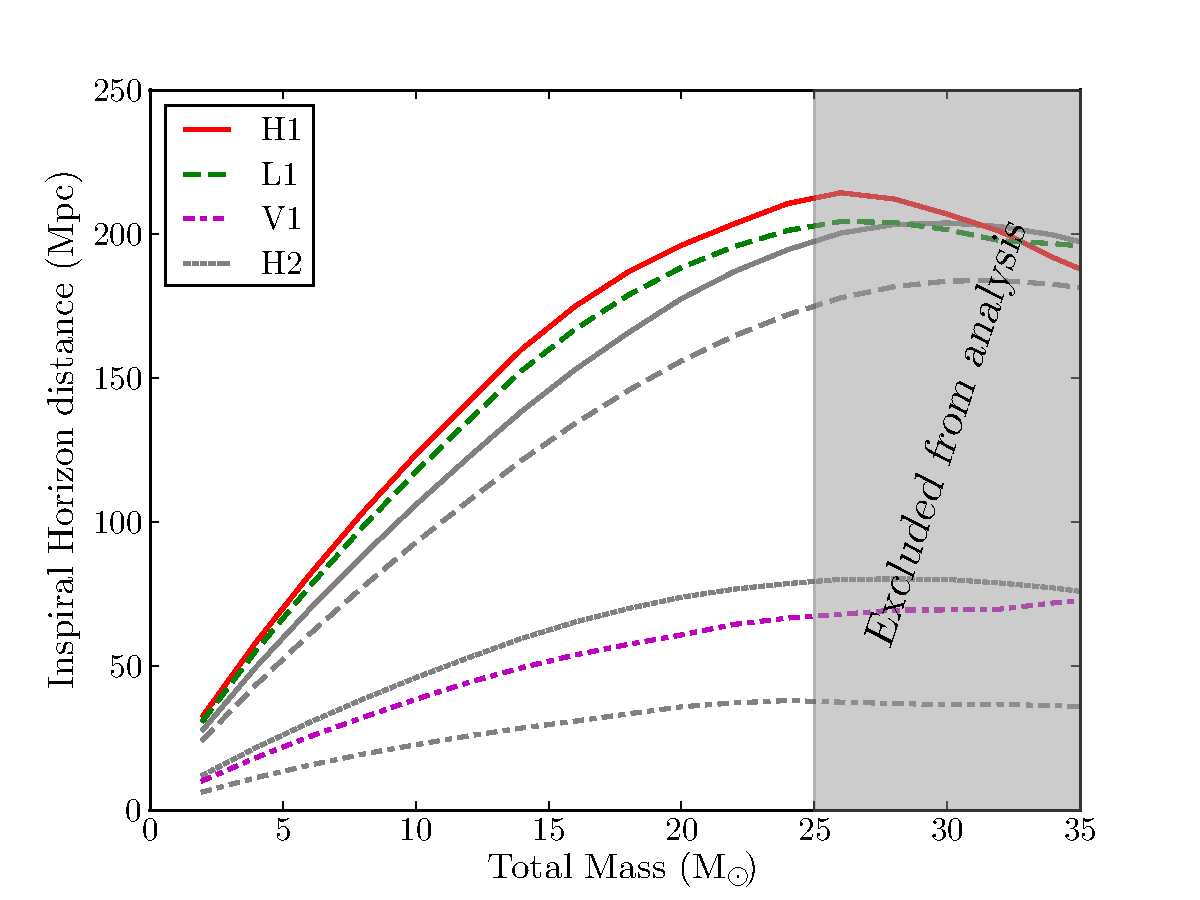
\includegraphics[width=6in]{figures/s6d_insprange_alt.pdf}
\end{center}
\caption{Average inspiral range of S6D. Shaded region indicates the mass range that was excluded in the low mass search for this period. Ranges were computed using the same method as in Figure \ref{fig:s6a_insprange}.}
\end{figure}

\begin{figure}[p]
\center
\subfigure[H1]{\includegraphics[width=3in]{figures/s6_clusterwin_investigation/H1_average_rate_per_tmplt_comparisons.png}}
\subfigure[L1]{\includegraphics[width=3in]{figures/s6_clusterwin_investigation/L1_average_rate_per_tmplt_comparisons.png}}
\subfigure[V1]{\includegraphics[width=3in]{figures/s6_clusterwin_investigation/V1_average_rate_per_tmplt_comparisons.png}}
\label{fig:avg_rate_per_tmplt}
\caption{The average trigger rate per template in week 3 of S6A as compared to one month from the \ac{S5} LV analysis. Each point represents a different stage in the pipeline: $0 \rightarrow$ \texttt{INSPIRAL\_FIRST}, $1 \rightarrow$ \texttt{THINCA\_FIRST}, $2 \rightarrow$ \texttt{INSPIRAL\_SECOND}, and $3 \rightarrow$ \texttt{THINCA\_SECOND}. Stages $4$--$7$ represent the higher-category vetoes being applied at \texttt{THINCA\_SECOND}; there is an extra stage in S6A because hardware injections were removed by an extra veto-category (between steps $5$ and $6$), whereas in the LV search hardware injections were removed as apart of the CAT2 vetoes (at step $4$).}
\end{figure}

\begin{figure}[p]
\label{fig:roc_cluster_windows}
\center
\includegraphics[width=6in]{figures/s6_clusterwin_investigation/s6week3cat4_ROC.png}
\caption{ROC plot from week 3 of S6A using various clustering windows and low-frequency cutoffs.}
\end{figure}

\section{DQ issues}

Review major DQ issues found through S6C and D studies.

\subsection{The ``Spike" Glitch}
Loud, short, transients in L1 OMC. Show one of Andy's time-series plots. Also show an Omega scan, and \ac{CBC} triggers created by it. Unable to determine cause. We resolved to create an \ac{SNR} > 250 flag, and veto at CAT3. Duncan MacCleod and I were supposed to study the effect on nearby injections, but it appears to have never finished.

\subsection{Decreasing the Upper End of the Template Bank}
High mass and low mass seraches overlapped in the region $25 \leq \mtotal/\Msun \leq 35$. Tom found that the high mass search did a better job recovering injections in this range. I did a study to see how much better the low-mass search would do with a smaller bank. Found that it was better, but not by enough to warrant re-doing runs up to that point. Show plotfm plots that I created. ROC curves?

During this investigation I find that nearby missed injection that appeared to be in clean time. Nothing became of it though; should I discuss this?

\subsection{V1 Doubles in S6D Triple Time}

V1 was glitchy and had poor range when came back up for VSR3. Summarize my study of what we gained/lost by throwing out H1V1 and L1V1 triggers in triple time. ROC plots? 

\section{Results}

Give loudest events. From re-runs? Copy from S6 paper?

\subsection{The Blind Injection}

Copy from S6 paper? Talk about extrapolation. Add detail about how extra slides were done. Remove discussion of parameter estimation.

\subsection{Conclusions}

In the S6 paper I draw on the upper-limits in the conclusion. Can I show preliminary upper limits?

\section{Extra Stuff}

(Next chapter)

The other investigation was the LIGO South investigation of whether or not we can detect at SNR 8 with two detectors. The wiki for this is linked from the April 13, 2010 CBC minutes. It was done using S5 data, so it doesn't seem to belong in this chapter. S5 chapter? Or at all? I allude to it in Chapter 2 we showing plots of snr and newsnr.



\Chapter{Can We Detect with Two Detectors? A Study for LIGO South}
\label{ch:ligo_south_study}
% ligo_south_study.tex

We currently plan to have three \ac{LIGO} detectors when Advanced LIGO comes online: one interfermeter at Livingston, L1, and two at Hanford: H1 and H2. H2 is planned to have $4\,$km arms, instead of the $2\,$km length it had in initial LIGO. However, in the past year the possibility opened up for a \ac{LIGO} interfermeter will be built in Australia. In this case, LIGO would still have three interferometers; rather than have two at Hanford, the optics for H2 would be shipped to the Australian site to be set up there.

\section{Advantages of LIGO South}

A number of studies were carried out to evaluate the pros and cons of having a H1L1S1 (S1 for the Austrialian detector) network as opposed to a H1H2L1 network. Most of these studies found that the H1L1S1 network had a number of advantages over the H1H2L1 network. Perhaps the biggest benefit is sources can be better localized if the third detector is in the southern hemisphere. Since the interferometers are not directional antennas, a network is needed to localize a source. Essentially, by measuring the difference in time of arrival between the various detectors in the network, we can triangulate the source (our brains do this to localize sounds, where the detectors are our ears). How well we can localize a source is given by \cite{ref:steve_triangulation_wiki, ref:localization_wiki}:
% localization_wiki: https://www.lsc-group.phys.uwm.edu/ligovirgo/cbcnote/aLIGOaVirgo/100223081702SouthLocalization%20through%20triangulation} 
\begin{equation*}
p(\mathbf{r}|\mathbf{R}) \propto p(\mathbf{r})\exp\left[ -\frac{1}{2}(\mathbf{r} - \mathbf{R})^T \mathbf{M}(\mathbf{r}-\mathbf{R})\right]
\end{equation*}
where $\mathbf{R}$ is the actual location, $\mathbf{r}$ is the reconstructed location, $p(\mathbf{r})$ is the prior distribution on $\mathbf{r}$, and $\mathbf{M}$ is given by:
\begin{equation*}
\mathbf{M} = \left[\sum \sigma_i^{-2}\right]^{-1} \sum_{i<j} \frac{\mathbf{D}_{ij}\mathbf{D}^T_{ij}}{\sigma^2_i \sigma^2_j}
\end{equation*}
Here, $\sigma_i$ is the timing accuracy in the $i\th$ detector and $\mathbf{D}_{ij}$ is the distance between the $i\th$ and $j\th$ detectors. Thus, the larger the distance between any two detectors, the more strongly peaked the probability distribution will be around the actual location.

It was found \cite{ref:steve_triangulation_wiki} that in the H1L1S1 network, an optimally located\footnote{Optimally located means the source is overhead the plane of the detector. The worst localization occurs when the source is in the plane of the detectors. The numbers presented are therefore best-case scenarios.} source at \ac{SNR} 7 could be localized to an area of $8.5$ square degrees with $90\%$ probability. In the H1H2L1 network the best localization was $12.5$ square degrees. If Virgo is added to the network, then with H1L1S1V1 the localization can be as small as $2.8$ square degrees with $90\%$ probability, whereas it is $10.0$ square degrees with H1H2L1V1.

Another advantage of an Australian detector, as opposed to two at Hanford, is all the detectors can be slid relative to each other. Recall that in \ac{S5} we could not analyze H1H2 time because of the correlated noise. Further, if there was some environmental factor that caused one of the Hanford detectors to lose lock, it would most likely also cause the other Hanford detector to lose lock. This hurt our duty cycle. If we instead have three non-co-located detectors, then we increase the probability that at least two detectors will be up at any given time, thereby increasing our total observation time.

\section{Can We Detect at SNR 8 with Two Detectors?}

There were a number of clear advantages to moving the second Hanford detector to Australia. However, one concern about doing this was the effect it would have on the Advanced LIGO projected chronology. If the optics for the second Hanford detector were packed up and shipped to Australia, it would likely take an additional two or more years to get the detector operational. This means that for the first few years of Advanced \ac{LIGO}, we would only have two detectors.\footnote{There is also the Virgo detector, but as Virgo is maintained and funded by a different collaboration, they may not have the same schedule as \ac{LIGO}. Thus, in this study we wanted to focus on what could be done with strictly the \ac{LIGO} detectors.} Our projected detection rates are based on being able to detect binaries at an \ac{SNR} of $8$. The concern was, if we only have two detectors, can we confidently detect a \ac{GW} at \ac{SNR} $8$? If we could not, then we would not build \ac{LIGO} South.

To answer this question we looked at the rates of H1L1 coincidences in \ac{S5}. We used \ac{S5} as opposed to \ac{S6} because \ac{S6} was still going on when we addressed this question. All of the months from the 12--18 month analysis were used, along with four months from the \ac{S5}-LV analysis. All H1L1 coincidences were used in double-, triple- and (in the case of the LV months) quadrupule- coincident times. For H1H2L1, H1L1V1, and H1H2L1V1 coincidences, the H1L1 part of the coincidence was used to re-calculate the combined new \ac{SNR} of the trigger.

Figure \ref{fig:ligo_south-cat3_newsnr} shows the result of the analysis for the low chirp-mass bin ($\mchirp < 3.48$). Plotted is the cumulative rate of zero-lag (``Foreground") and slide (``Background") triggers as a function of combined new \ac{SNR}. The slide triggers were generated from the standard 100-slide \ihope analysis. The y-axis was generated in the same manner as in the cumulative-rate plots in Figures \ref{fig:} of Chapter \ref{ch:s6_results}. Indeed, these plots were a predecessor to the rate plots shown in Chapter \ref{ch:s6_results}. The dashed-red line shows what the combined new \ac{SNR} would be for signal with \ac{SNR} $8$ in each detector ($= 11.3$). Also plotted, as a yellow star, is the combined new \ac{SNR} of a blind \ac{CBC} injection that was made during \ac{S5}. (This injection, which was in the \ac{S5}-LV analysis, was missed because it occurred when an earthquake was passing Livingston, resulting in L1 being CAT3 vetoed during the time. For more details on this blind injection, see \cite{ref:s5LV}.)

It is evident from the plot that an event with a new \ac{SNR} of $8$ in each detector would stick out above the background. In this case, we would place an upper-limit on the \ac{FAR} as being $< 1$ in $50$ years. We can arrive at the same conclusion from looking at Figure \ref{fig:?} of Chapter \ref{ch:s6_results}. (Recall that these plots were also created using only H1L1 triggers.) There we can use the extrapolation to estimate what the \ac{FAR} would be for an signal with combined new \ac{SNR} of $11.3$. In the low chirp-mass bin we would have a \ac{FAR} $\approx 1$ in $10^4$ years. 

\subsection{Caveats}

There are a few caveats to this analysis. First, note that we have shown results after CAT3 vetoes have been applied. Figure \ref{fig:ligo_south-newsnr_cat2} shows the same plot as in Figure \ref{fig:ligo_south-money_plot} after CAT2 vetoes have been applied. In this plot we can see that an event at \ac{SNR} $8$ in each detector \emph{would not} stick above the background; it would only have a \ac{FAR} of $\sim1$ in $3$ years. This highlights the importance of \ac{DQ} investigations. Without good data-quality, we cannot detect at \ac{SNR} $8$ using two detectors.

Second, note that we have plotted results as a function of combined \emph{new} \ac{SNR}. Figure \ref{fig:ligo_south-snr_cat3} shows the results after CAT3 as a function of combined \ac{SNR}. The large tail due to non-Gaussian transients has buried the \ac{SNR} 8/8 line in background; such an event would have a \ac{FAR} of $\sim1$ in $30$ years if combined \ac{SNR} was our ranking statistic. Clearly, without new \ac{SNR} we could not detect at \ac{SNR} $8$ (or $40$, for that matter). However, when talking about real events, we have interchanged new \ac{SNR} and \ac{SNR}: we quote rates based on a \emph{\ac{SNR}} of $8$ in each detector, yet we have placed the red-dashed line at a \emph{new \ac{SNR}} of $8$ in each detector. The reason we can do this is new \ac{SNR} reduces to \ac{SNR} for (well-modelled) \acp{GW}. Figure \ref{fig:ligo_south-newsnr_v_snr} shows a plot of combined new \ac{SNR} versus combined \ac{SNR} for (non-spinning) injections. The vertical dashed line shows the combined $\rho = 11.3$ point. At this point, we can see that most of the injections have a combined new \ac{SNR} $> 11$. Note that some of the lower points are due to glitches being mistakenly mapped to injections; c.f. Figure \ref{fig:ligo_south-inj_mchirp_accuracy}. Thus to detect with two detectors at the quoted rates, we need new \ac{SNR}, which in-turn requires that we have templates the well-match the \ac{GW} signal.

Finally, note that we have so far only shown plots for the low chirp-mass bin. The background does not fall off as sharply in the higher chirp-mass bins. This can be seen by comparing Figure \ref{fig:?} to Figure \ref{fig:?}: the medium chirp-mass bin has a higher tail, leading to larger \acp{FAR} at the same new \ac{SNR}. However, as can be seen in the extended background with the blind injection removed (the gray crosses) in Figure \ref{fig:?}, we would still get a \ac{FAR} of $~1$ in $3500$ years in the medium chirp-mass bin at a combined new \ac{SNR} $11.3$. Though higher than the low chirp-mass bin, this \ac{FAR} is still low enough to claim evidence for a detection. Further, we are most concerned with the low chirp-mass bin, as this contains \ac{BNS} systems. Out of \ac{BNS}, \ac{BBH} and \ac{NSBH} systems, the rate of \ac{BNS} coalescence in the universe is the best constrained, as it is based on actual astrophysical observations of \ac{BNS} systems. We are therefore most confident in quoted expected rates of detection for \ac{BNS} coalescence, and so it is for these systems that we wish to ensure that we can detect at \ac{SNR} 8.

\section{Conclusions}

This study showed that building \ac{LIGO} South would not hamper our abilities to detect \ac{GW} at the quoted rates in the near term. Thus the decision of whether or not to build \ac{LIGO} South can be based solely on the availability of funds. Regardless of whether or not \ac{LIGO} South is built, this study proved useful, as it gave us confidence that we can detect \acp{GW} at expected rates in Advanced LIGO. Admittedly, we cannot be certain that the character of the noise will be the same in Advanced LIGO. However, by comparing the \ac{S5} cumulative rate plot in this chapter to the corresponding \ac{S6} plots in Chapter \ref{ch:s6_results}, we see that we obtained largely the same (better, even) background distribution in \ac{S6}, despite a number of hardware differences between the runs. Thus, by making using of new \ac{SNR}, and with equally intensive \ac{DQ} studies in Advanced \ac{LIGO}, we can expect to detect at a \ac{SNR} of $8$ in each detector.

\begin{figure}[p]
\center
\includegraphics[width=6in]{figures/ligo_south/Cat3-newsnr-low_mass.png}
\label{fig:ligo_south-cat3_newsnr}
\caption{Cumulative rate of H1L1 zero-lag (``Foreground") and slide (``Background") coincidences in \ac{S5} after CAT3 (cumulative) vetoes have been applied. Only triggers in the low chirp-mass bin ($\mchirp < 3.48\,\Msun$) are shown. Data used is from all of the \ac{S5} 12-18 months, plus four months from the \ac{S5}-LV analysis. The black line indicates the background; the blue line indicates the foreground. As with the cumulative rate plots in Chapter \ref{ch:s6_results}, the foreground rates are computed by dividing the cumulative count of foreground triggers by the total zero-lag live time ($T_{\mathrm{f}}$). The background rates are computed by dividing the cumulative count of background triggers by total slide live time ($T_{\mathrm{b}}$), which is equivalent to divding by the effective number of slides ($= T_{b}/T_{f}$), then dividing by the zero-lag live time. Hence the black line is labelled as the ``Average Background." The red-dashed line indicates the combined new \ac{SNR} for an event with single-\ac{IFO} new \ac{SNR} of $8$ in each detector. The yellow star shows the combined new \ac{SNR} of a blind injection that was made during the \ac{S5}-LV analysis.}
\end{figure}

\begin{figure}[p]
\center
\subfigure[After CAT2 vetoes applied.]{\label{fig:ligo_south-newsnr_cat2}\includegraphics[height=3.5in]{figures/ligo_south/Cat2-newsnr-low_mass.png}}
\subfigure[Cumulative rate vs. combined \ac{SNR}, after CAT3 vetoes applied.]{\label{fig:ligo_south-snr_cat3}\includegraphics[height=3.5in]{figures/ligo_south/Cat3-snr-low_mass.png}}
\label{fig:ligo_south-cat2_and_snr}
\caption{Cumulative rate plot for the same period of time shown in Figure \ref{fig:ligo_south-cat3_newsnr}, after CAT2 vetoes have been applied (top) and as a function of combined \ac{SNR} (bottom). In the bottom plot, CAT3 vetoes have been applied.}
\end{figure}

\begin{figure}[p]
\center
\includegraphics[width=6in]{figures/ligo_south/H1L1-ligolw_cbc_plotfm_Non-Spinning_mathcalM_mathrminj_0_3_F1_BNSLININJ+BNSLOGINJ+NSBHLININJ+NSBHLOGINJ+BBHLININJ+BBHLOGINJ_PLOTTED-961545543-3628944.png}
\label{fig:ligo_south-newsnr_v_snr}
\caption{Combined new \ac{SNR} versus combined \ac{SNR} for non-spinning injections. All injections were found as H1L1 coincidences. Results taken from $6$ weeks of S6D data. The diagonal black-dashed line indicates $y=x$; the vertical dashed line shows the point where combined \ac{SNR} $= 11.3$. This plot was created by \texttt{ligolw\_cbc\_plotfm}. As with all PlotFM plots, the blue stars indicate injections found with $0$ \ac{FAR} in their analysis period and colored circles indicate injections with non-zero \ac{FAR}.}
\end{figure}

\begin{figure}[p]
\center
\includegraphics[width=6in]{figures/ligo_south/H1L1-ligolw_cbc_plotfm_Non-Spinning_frac_accuracy_mathcalM_mathrminjected_0_3_F3_BNSLININJ+BNSLOGINJ+NSBHLININJ+NSBHLOGINJ+BBHLININJ+BBHLOGINJ_PLOTTED-961545543-3628944.png}
\label{fig:ligo_south-inj_mchirp_accuracy}
\caption{Recovered chirp mass fractional accuracy of the injections shown in Figure \ref{fig:ligo_south-newsnr_v_snr} as a function of combined \ac{SNR}. Triggers close to zero were most likely caused by injections. Triggers further from the zero line are most likely glitches that happened to be within $\pm 1\,$s of the injection.}
\end{figure}


\Chapter{Future Developments and Conclusions}
\label{ch:future_developments}
% future_developements.tex

We have stepped through, in detail, the low-mass \ac{CBC} pipeline, and we have described how this was used to obtain search results. We now conclude by briefly presenting some future developements for the pipeline.

\section{Gating}

In chapter \ref{ch:s6_results} we saw the effects a loud transient --- the spike glitch --- had on the matched filter. We dealt with the spike glitch by adding a category 3 veto around the time of the glitch. Due to the ringing of the filter we had to add a $\pm 8\,$s padding to the glitch. However, as can be seen in figure \ref{fig:spike_glitch-cbc_response}, triggers can be last for several tens of seconds after the glitch; this duration increases with the size of the glitch.

Another possiblity is to remove the glitch \emph{prior} to match filtering. We can do this by applying a Tukey window to the data stream to ramp the output down to $0$ at the time of the glitch. We call this ``gating." Figure \ref{fig:gating-time_series} shows a time series in which a spike-glitch occurred with a gate applied.  In \ref{fig:gating-time_series-gated} the window that is applied can be seen. We must ramp the data down (in this case, by using the first half cycle of a cosine) so as not to introduce ringing at the point the window turns on, and we must do the same after the glitch to ramp the data back up. In this manner we can cleanly remove the glitch from the data: compare the Omega scans in figure \ref{fig:gating-omega_scans} with the glitch in to the scan with the glitch out.

Zeroing out the data around the glitch does mean that we will slightly underestimate the \ac{PSD}. However, if the gated data is only a few seconds out of an entire analaysis chunk, the effect should be small. It may also be possible to correct for the zeroed out data by taking the average power across the segment, then add a correction factor. Even if we add a correction factor to the \ac{PSD}, we should probably limit the amount of time that is gated in an analysis chunk. The upper limit on how much time can gated in a chunk requires more study.

Knowing what to gate also needs study. In the case of the spike glitch, we could not find the cause, as we could not correlate it with any ``safe" channel. We got around this difficulty by applying the \ac{SNR} $> 250$ flag at CAT3, which allowed us to check the results at CAT2 to ensure we did not accidently veto a loud \ac{GW} triggers. Since gating involves removing the glitch before filtering, we would not have that luxury, unless we were to match filter the data multiple times. Another possibility is to establish a \ac{SNR} for which burst searches do as-good-as \ac{CBC} searches at finding \ac{GW} signals. We would then remove any trigger that exceeded that threshold, leaving it to the burst, or a mixed burst-\ac{CBC} search to find loud triggers. Finding that threshold, and determining the safety of such a scheme, is yet to be done.

\begin{figure}[p]
\center
\subfigure[Raw time series.]{\label{fig:gating-time_series-raw}\includegraphics[width=4.75in]{figures/gating/time_series-spike.png}}
\subfigure[Gated time series.]{\label{fig:gating-time_series-gated}\includegraphics[width=4.75in]{figures/gating/time_series-gated.png}}
\caption{Raw and gated time series of a L1 spike glitch that occurred during \ac{S6}. In the raw time series (top) we can see that this was actually two glitches in quick succession. For this reason, the gate was chosen to be $\pm1.5s$ around the larger glitch. The effect of the ramping down of the Tukey window can be seen in the gated time-series.}
\label{fig:gating-time_series}
\end{figure}

\begin{figure}[p]
\center
\subfigure[Scan with glitch in.]{\label{fig:gating-omega_scan-raw}\includegraphics[width=4.75in]{figures/gating/omega_scan-spike.png}}
\subfigure[Scan with gate.]{\label{fig:gating-omega_scan-gated}\includegraphics[width=4.75in]{figures/gating/omega_scan-gated.png}}
\caption{Omega scan of the spike glitch shown in figure \ref{fig:gating-time_series}. The top plot shows the scan with the glitch in the data; the bottom plot shows the scan with the glitch removed. Omega applies a whitening filter when these scans are generated. The ringing of the filter is evident in the top plot. With the glitch gated, we see that there is no ringing.}
\label{fig:gating-omega_scans}
\end{figure}

\section{Single Stage Pipeline and Updates to Pipedown}

Using a two stage-pipeline, as presented in chapter \ref{ch:ihope_pipeline}, makes it difficult to followup triggers, and to do things such as perform more slides, as dicussed in chapter \ref{ch:s6_results}. \ac{HIPE} was developed to have two stages in order to save on the computational cost of calculating $\chi^2$. This was done several years ago. Since then, advancements in computing speed have made it possible to use a \emph{single-stage} pipeline. In this, $\chi^2$ is calculated at first inspiral, and so no second stage is needed. Having such a pipeline would make it far simplier to followup triggers and to know how they evolve through the pipeline.

As mentioned in \ref{ch:s6_results} a prototype single-stage pipeline already exists. Some updates need to be made to Pipedown to be able to use this pipeline, however, as some of the programs rely on conventions of the current \ac{HIPE} pipeline. Of note: in the singe-stage pipeline, \verb|lalapps_thinca| is replaced by an updated verison, \verb|ligolw_thinca|, which natively makes use of the Coinc and Experiment tables discussed in chapter \ref{ch:ihope_pipeline}. It also performs linear slides as opposed to slides on a ring. This removes the need for \verb|ligolw_thinca_to_coinc| in Pipedown.

A few other improvements are also planned for Pipedown. As mentioned in Chapter \ref{ch:ihope_pipeline}, multiple veto categories can be stored in a single database. Pipedown currently does not take advantage of this. As part of the switch to a single-stage pipeline, we plan to add a program to Pipedown to apply vetoes in the database, so as not to have to run \verb|ligolw_thinca| multiple times. Also, a number of programs in Pipedown cannot read data from multiple databases. This makes it difficult to combine results from multiple runs. Reading from multiple databases will require a slight update to the \verb|experiment| table. Namely, we plan to replace the \verb|gps_start| and \verb|gps_stop| columns with a \verb|segment_def_id| column. This would point to a list of segments in the \verb|segment| and \verb|segment_definer| tables that give the analyzed time covered by the database.

Pipedown can also be greatly simplified. Currently, it has to create intermediate databases that separately store injection data from each of the runs. These \verb|RAW| databases lack much information, such as the vetoes applied and the livetime. This is done so as to limit the size of the xml files that need to be extracted for \verb|lalapps_inspinjfind|. Since clustering is done on these intermediate databases it makes it difficult to test new statistics. If one wants to cluster with the new statistic, they must re-run clustering on all of the individual \verb|RAW| databases, carry out injection-finding, create a new final database, and re-compute the livetime. If \verb|lalapps_inspinjfind| could read databases instead, all of the injection runs could be added to the \verb|FULL_DATA RAW| database at the outset, greatly simplifying the pipeline and the ability to test new statistics. Work on this is planned. Along with this update to the injection finding program, we plan to implement more sophisticated injection finding techniques, such as using ethinca windows.

Finally, note that out of all the tables Pipedown makes use of, only the \verb|coinc_inspiral| and \verb|sngl_inspiral| are specific to the low-mass \ac{CBC} search. All mappings between the Experiment --- which can be used for any search --- and the other Coinc tables are based on the \verb|coinc_event_id|. Thus, if another search uses tables that are equivalent to \verb|sngl_inspiral| and \verb|coinc_inspiral| tables, all these tables need are a \verb|event_id| column and a \verb|coinc_event_id| column and they can make use of the same architecture. All the programs run by Pipedown could then run on any search; we just need to swap out pointers to the \verb|coinc_inspiral| and \verb|sngl_inspiral| table for more generic names that could be set in the configuration file. We have done just that for the \ac{CBC} group's \emph{ringdown} search. This search looks for \acp{GW} emitted by black holes after they coalesce and are ``ringing down." This search stores its single-\ac{IFO} in a \verb|sngl_ringdown| table and its coincident data in a \verb|coinc_ringdown| table, which have \verb|event_id| and \verb|coinc_event_id| columns, respectively. A prototype of Pipedown has been developed that takes the table-names from the configuration file. By simply changing the parameters in the configuration file, we have been able to run Pipedown on this search. This update is currently being tested.

%\section{Calculating False Alarm Rates from Single IFO Distributions}
%
%As we saw in chapter \ref{ch:s6_results}, the presence of a signal in the data --- in our case, it was a blind injection --- can alter the background estimation for that trigger. We saw why this happens in equation \ref{eqn:slideTerms} in Chapter \ref{ch:far}: if the probability is high that a signal exists in the data, it mixes with the noise triggers to increase the background estimate. This problem is compounded if there are multiple signals in the data, as may be the case in advanced \ac{LIGO}.
%
%One possibility to deal with this is to remove the single-\ac{IFO} triggers associated with a given foreground coincidence from the slides when computing the false alarm rate for that trigger. We pioneered this in \ac{S6} when we estimated the false alarm rate for the blind injection. However, concerns arose that if the blind injection were from noise, we would underestimate its \ac{FAR}.
%
%Another possibility is suggested by equation \ref{eqn:exptd_slid_coincs}. If we fit a probability distribution in new \ac{SNR} of the single-\ac{IFO} triggers (before coincidence testing), we could get a false alarm rate by performing the integral in \ref{eqn:exptd_slid_coincs}, with the \ac{GW} term set to zero. Although a signal may exist in the data, the fit would be less suscepitible to its influence than time slides, since, persumably, the number of signals would be far less than the number of noise triggers. The difficulty in this method is establishing what distribution to use. Although new \ac{SNR} removes most of the non-Gaussian tail, it is not clear that resulting distribution should be $\chi^2$ distributed with two degrees of freedom. Further, a 

\section{Conclusion}

The data-analysis methods, pipeline, and search results presented in this thesis are the result of years of work by a number of people throughout the \ac{LSC} and the Virgo Collaboration. Although no gravitational-waves have been detected as of yet, injection studies, comparisons of our upper-limits to astrophysical predictions, and the result of the \ac{S6} blind injection challenge have made us confident that we will be able to detect when advanced \ac{LIGO} and Virgo come online. The work to build advanced \ac{LIGO} is currently underway. When it is finished it will present new challenges to our data analysis pipeline, some of which are outlined here. In the coming years we will continue to improve and refine our analysis techniques to meet those challenges, so that, when an event happens, we will detect it.


\clearpage
\bibliographystyle{unsrt}
\bibliography{references}
\addcontentsline{toc}{chapter}{\numberline {Bibliography}}

\clearpage
\birthplacedate{Glens Falls, New York \>\>February 15, 1983}
\collegewherewhen{
\>Syracuse University \>\>B.S. Physics, 2005\\
\>Syracuse University \>\>M.S. Physics, 2008}

\newpage
\null%\vskip1in%
\begin{center}
{\Large\bf Curriculum Vitae}
\end{center}
%\vskip 2em
%\begin{tabbing}
%\tabset
%Title of Dissertation\\
%\>Searching for Gravitational Radiation from Compact Binary
%Coalescence Using LIGO and Virgo Data
%\end{tabbing}
%\vskip 1em

\begin{startvita}
\end{startvita}

\renewenvironment{thebibliography}[1]%
  {\begin{list}{\labelenumi\hss}%
     {\usecounter{enumi}\setlength{\labelwidth}{3em}%
      \setlength{\leftmargin}{5em}}}%
  {\end{list}}
\renewcommand{\bibitem}[1]{\item\label{#1}\relax}%
\renewcommand{\theenumi}{\arabic{enumi}}%
\begin{publications}
\putbib[papers]
\end{publications}

\begin{honorarysocieties}
2001 \>Syracuse University Founders' Scholarship\\
\end{honorarysocieties}

%\finishvita

% The grad school requires the last page to be blank
\newpage
\thispagestyle{empty}
\mbox{}
\end{document}
